% PPGEE - UFMG
%-------------------------------------------------------------------

% Definies gerais do documento 

\documentclass[12pt,a4paper,titlepage]{book}
% \documentclass[12pt,a4paper,titlepage,final]{book}
% \documentclass[12pt,a4paper,titlepage,brazil,portugues]{book}
%--------------------------------------------------------------------
% \usepackage[left=2.5cm,right=2.5cm,top=4cm,bottom=2.5cm]{geometry}
\usepackage[left=1.5cm,right=3.5cm,top=4cm,bottom=2.5cm]{geometry}
%--------------------------------------------------------------------
% Pacotes usados {{
\usepackage[utf8]{inputenc}
\usepackage[T1]{fontenc}
\usepackage{amsmath,amssymb,amsfonts,amstext,textcomp}         % permite simbolos matematicos
\usepackage{bm}                                                % negrito em letras gregas
\usepackage{mathrsfs}                                          % permite o uso de letras trabalhadas
\usepackage{amsthm}
\usepackage{pgf}
\usepackage{graphicx}
\usepackage{float} % Allows putting an [H] in \begin{figure} to specify the exact location of the figure
\usepackage{color}
\usepackage{xcolor}
\usepackage{booktabs}                                          % Tabelas com qualidade de publicao
\usepackage{indentfirst}
\usepackage{rotating}
\usepackage{braket}
\usepackage[ruled,vlined]{algorithm2e}                         % Para algoritmos (melhor que o outro)
\usepackage{multirow}
\usepackage{fancyhdr}
\usepackage{makeidx}
\usepackage{setspace}
\usepackage[colorlinks,citecolor=blue]{hyperref}               % tirar [colorlinks] para imprimir
\usepackage{ae}
\usepackage[below]{placeins}
\usepackage{flafter}
\usepackage{pxfonts}
% \usepackage{subfigure}
\usepackage{appendix}
\usepackage{listings}                                          % para cdigo fonte
\usepackage[symbol]{footmisc}                                  % Mudando marcadores do footnote
\usepackage{tikz}
      \usetikzlibrary{shapes,arrows,calc,automata,positioning}
\usepackage{soul}                                              % para highlighth (todonotes)
\usepackage{natbib}                                            % para usar citep, etc...
\usepackage{subfig}                                            % para usar citep, etc...
\usepackage[
      textsize=scriptsize,
      colorinlistoftodos,
      % shadow,
      color=yellow,
      backgroundcolor=yellow,
      % obeyDraft
      obeyFinal
      ]{todonotes}
% \usepackage[
      % natbib=true,
      % % citestyle=authoryear,
      % citestyle=rusnat,
      % % bibstyle=authortitle,
      % % style=authoryear-comp,
      % hyperref=true,
      % backend=biber,
      % maxbibnames=99,
      % giveninits=true,
      % uniquename=init,
      % maxcitenames=2,
      % parentracker=true,
      % url=false,
      % doi=false,
      % isbn=false,
      % eprint=false,
      % backref=true]{biblatex}
% \usepackage[style    = abnt,           % Sistema alfabetico
          % % style    = abnt-numeric,   % Sistema numerico
          % % style    = abnt-ibid,      % Notas de referencia]{biblatex}
% ]{biblatex}
% \usepackage{mcode}
% \usepackage{amssymb}
% \usepackage{amsmath}
% \usepackage{caligra} %letras caligraficas
% \usepackage{caligr}%letras caligraficas
% \usepackage{dsfont}%barra escura para conjuntos
% \usepackage[dvips]{graphicx}
% \thispagestyle{empty}
% \usepackage{epsfig,latexsym}
% \usepackage{psfrag}
% \usepackage{epsfig}
% \usepackage[siunitx]{circuitikz} % fazer diagramas de blocos
% \usepackage{algorithm}
% \usepackage[noend]{algpseudocode}   % Para pseudo-codigos
% \usepackage[linesnumbered,ruled,vlined]{algorithm2e} % Para algoritmos (melhor que o outro)
% \usepackage[pdftex]{hyperref}
% \usepackage[hang,small]{caption}
% \usepackage{icomma}

% Para nao sobrar espaos em branco estranhos
% \widowpenalty=1000 \clubpenalty=1000
% \newcommand{\gepeto}[1]{\vspace*{12pt}\begin{singlespace}\hspace{2cm}\begin{small}\parbox{12cm}{#1}\end{small}\end{singlespace}\vspace*{20pt}}


\theoremstyle{definition}
\newtheorem{theorem}{Theorem}[section]
\newtheorem{corollary}{Corollary}[theorem]
\newtheorem{lemma}[theorem]{Lemma}
% \newtheorem{defi}{Definio}[section]
% \newtheorem{propo}{Proposio}[section]
% \newtheorem{coro}{Corolrio}[section]
% \newtheorem{exem}{Exemplo}[section]
% \newtheorem{lema}{Lema}[section]
% \newtheorem{consi}{Considerao}[section]


% Modificacoes em legenda
\setlength{\belowcaptionskip}{10pt}
% \addbibsource{referencias.bib}

% {{{ Modificas em legenda (quando ocorre quebra das palavras indesejadas)
% \hyphenation{na-tu-ra-is}
% \hyphenation{ge-ra-do}

% {{{ Definicao de comandos

\newcommand{\comment}[1]{}
\newcommand{\veq}{\vspace{0.2cm}}
\newcommand{\x}{\\[5pt]}
\newcommand{\C}[1]{\relax}

\newtheorem{teo}{Theorem}[section]
\newtheorem{defin}[teo]{Definition}
\newtheorem{nota}{Note}[section]

% }}}

% {{{ Novos operadores
\DeclareMathOperator*{\argmax}{argmax}
\DeclareMathOperator*{\argmin}{argmin}
% }}}

% {{{ Captulo personalizado
\makeatletter
\def\thickhrulefill{\leavevmode \leaders \hrule height 1ex \hfill \kern \z@}
\def\@makechapterhead#1{%
  \vspace*{10\p@}%
  {\parindent \z@ \centering \reset@font
        \thickhrulefill\quad
        \bfseries \@chapapp{} \thechapter
        \quad \thickhrulefill
        \par\nobreak
        \vspace*{10\p@}%
        \interlinepenalty\@M
        \hrule
        \vspace*{10\p@}%
        \Huge \bfseries #1\par\nobreak
        \par
        \vspace*{10\p@}%
        \hrule
    \vskip 70\p@    %100
  }}
\def\@makeschapterhead#1{%
  \vspace*{10\p@}%
  {\parindent \z@ \centering \reset@font
        \thickhrulefill
        \par\nobreak
        \vspace*{10\p@}%
        \interlinepenalty\@M
        \hrule
        \vspace*{10\p@}%
        \Huge \bfseries #1\par\nobreak
        \par
        \vspace*{10\p@}%
        \hrule
    \vskip 70\p@
 }
}
% }}}

%--------------------------------------------------------------------
%Variacao da altura da linha
\renewcommand{\baselinestretch}{1.1}

%--------------------------------------------------------------------
%Coloca Rascunho e a data
\newcommand{\reviewtimetoday}[2]{\special{!userdict begin
/bop-hook{gsave 20 710 translate 45 rotate 0.8 0.8 0.8 0.8 0 setcmykcolor
/Times-Roman findfont 10 scalefont setfont 0 0   moveto (#1) show
0 -12 moveto (#2) show grestore}def end}}
% You can turn on or off this option.
\reviewtimetoday{\today}{Draft Version}

%--------------------------------------------------------------------
%Criar o index
\makeindex

%--------------------------------------------------------------------
%Devido ao fancyheading
\headheight 14.7pt

%--------------------------------------------------------------------
%Trocando os efeitos da virgula e ponto
% \DeclareMathSymbol{,}{\mathord}{letters}{"3B}
% \DeclareMathSymbol{.}{\mathpunct}{letters}{"3A}

% -*- TeX-master: "Qualificacao.tex" -*-
%!TEX root = Qualificacao.tex

\newcommand{\norm}[1]{\left\lVert#1\right\rVert}

%%%%%%%%%%%%%%%%%%%%%%%%%%%%%%%%%%%%%%%%%%%%%%%%%%%%%%%%%%%%%%%%%%%%%%%
%                    Theorems, definitions, etc...                    %
%%%%%%%%%%%%%%%%%%%%%%%%%%%%%%%%%%%%%%%%%%%%%%%%%%%%%%%%%%%%%%%%%%%%%%%


\theoremstyle{plain}
\newtheorem{thm}{Theorem}[section]
\newtheorem{lem}[thm]{Lemma}
\newtheorem{prop}[thm]{Proposition}
\newtheorem*{cor}{Corollary}

\theoremstyle{definition}
\newtheorem{defn}{Definition}[chapter]
\newtheorem{assum}{Assumption}[chapter]
\newtheorem{conj}{Conjecture}[section]
\newtheorem{exmp}{Example}[section]

\theoremstyle{remark}
\newtheorem*{rem}{Remark}
\newtheorem*{note}{Note}

%%%%%%%%%%%%%%%%%%%%%%%%%%%%%%%%%%%%%%%%%%%%%%%%%%%%%%%%%%%%%%%%%%%%%%%
%                               Vectors                               %
%%%%%%%%%%%%%%%%%%%%%%%%%%%%%%%%%%%%%%%%%%%%%%%%%%%%%%%%%%%%%%%%%%%%%%%

\newcommand{\vet}[1]{\mathrm{\mathbf{#1}}}
\newcommand{\vx}{\vet{x}}
\newcommand{\vX}{\vet{X}}
% \newcommand{\vu}{\vet{u}}
\newcommand{\vu}{u}
\newcommand{\vy}{\vet{y}}
\newcommand{\vA}{\vet{A}}
\newcommand{\vB}{\vet{B}}
\newcommand{\vG}{\vet{G}}
\newcommand{\vH}{\vet{H}}
\newcommand{\vC}{\vet{C}}
\newcommand{\vD}{\vet{D}}
\newcommand{\vQ}{\vet{Q}}
\newcommand{\vR}{\vet{R}}
\newcommand{\vt}{\bm{\theta}}
\newcommand{\vf}{\vet{f}}
\newcommand{\vg}{\vet{g}}
\newcommand{\vK}{\vet{K}}
\newcommand{\vP}{\vet{P}}
\newcommand{\vv}{\vet{v}}
\newcommand{\vw}{\vet{w}}

\newcommand{\vtheta}{\bm{\theta}}
\newcommand{\vepsilon}{\bm{\epsilon}}
\newcommand{\vvarphi}{\bm{\varphi}}
\newcommand{\vPhi}{\bm{\Phi}}
\newcommand{\vPsi}{\bm{\Psi}}
\newcommand{\vxi}{\bm{\xi}}
\newcommand{\vmu}{\bm{\mu}}
\newcommand{\vpi}{\bm{\pi}}


%%%%%%%%%%%%%%%%%%%%%%%%%%%%%%%%%%%%%%%%%%%%%%%%%%%%%%%%%%%%%%%%%%%%%%%
%                        Virtual Signals                              %
%%%%%%%%%%%%%%%%%%%%%%%%%%%%%%%%%%%%%%%%%%%%%%%%%%%%%%%%%%%%%%%%%%%%%%%

\newcommand{\rv}{\bar{r}}
\newcommand{\ev}{\bar{e}}


%%%%%%%%%%%%%%%%%%%%%%%%%%%%%%%%%%%%%%%%%%%%%%%%%%%%%%%%%%%%%%%%%%%%%%%
%                            Other symbols                            %
%%%%%%%%%%%%%%%%%%%%%%%%%%%%%%%%%%%%%%%%%%%%%%%%%%%%%%%%%%%%%%%%%%%%%%%

\newcommand{\E}{\mathbb{E}}
\newcommand{\Prob}{\mathbb{P}}
\newcommand{\R}{\mathbb{R}}

\newcommand{\pt}{\tilde{\phi}}
\newcommand{\ph}{\hat{\phi}}

\newcommand{\Wh}[1]{\hat{W}_{#1}}
\newcommand{\Wht}[1]{\hat{W}_{#1}^T}
\newcommand{\Wt}[1]{\tilde{W}_{#1}}
\newcommand{\Wtt}[1]{\tilde{W}_{#1}^T}

\newcommand{\Wio}{W_i^*}
\newcommand{\Wiot}{W_i^{*T}}

\newcommand{\Wci}{\hat{W}_{ci}}
\newcommand{\Wai}{\hat{W}_{ai}}
\newcommand{\Wcit}{\hat{W}_{ci}^T}
\newcommand{\Wait}{\hat{W}_{ai}^T}

\newcommand{\laplace}[1]{\mathcal{L} \left\{ #1 \right\}}
\newcommand{\realiz}{$(A, B, C, D)$ }
\newcommand{\eqpar}[2]{\frac{\partial{#1}}{\partial{#2}}}

\newcommand{\xb}{\bar{x}}
% \newcommand{\norm}[1]{||#1||}
\newcommand{\Sb}{\bar{S}}

\newcommand{\Jio}{J_i^*}
\newcommand{\Jiz}{J_i^0}
\newcommand{\Jiho}{\hat{J}_i^*}

% \newcommand{\vpfa}{\mathbf{\phi}}

% Function approximations
\newcommand{\vpfa}{\bm{\varphi}}
\newcommand{\pfa}{\phi}
\newcommand{\Jfa}{\hat{J}}
\newcommand{\Jfaxp}{\hat{J}(\vx,\vpfa)}
\newcommand{\Jfaxpk}{\hat{J}(\vx_k,\vpfa_k)}
\newcommand{\Qfa}{\hat{Q}}
\newcommand{\Qfaxp}{\hat{Q}(\vx,u,\pfa)}

% Policy Gradient Methods
\newcommand{\apPG}{\nabla \hat{P}(\vt_k)}


\newcommand{\vuo}{\alpha_1^*}
\newcommand{\vuh}{\hat{\alpha}_1}
\newcommand{\vi}{\alpha_i}
\newcommand{\vio}{\alpha_i^*}
\newcommand{\viho}{\hat{\alpha}_i^*}
\newcommand{\vih}{\hat{\alpha}_i}
\newcommand{\vnh}{\hat{\alpha}_n}
\newcommand{\vnah}{\hat{\alpha}_{n-1}}
\newcommand{\vnahd}{\dot{\hat{\alpha}}_{n-1}}
\newcommand{\viah}{\hat{\alpha}_{i-1}}
\newcommand{\viahd}{\dot{\hat{\alpha}}_{i-1}}
\newcommand{\viaahd}{\dot{\hat{\alpha}}_{i-2}}


\newcommand{\tq}{\tilde{Q}}
\newcommand{\tqxu}{\tilde{Q}(x_k,u_k)}
\newcommand{\tqxuo}{\tilde{Q}(x_{k+1},u_{k+1})}



% Define a counter for the inserted todonotes.
\newcounter{todoListItems}
% \newcommand{\todoTrans}[2]{
% % Increment counter
% \addtocounter{todoListItems}{1}
% \todo[%
% caption={\protect\hypertarget{todo\thetodoListItems}{}[\thetodoListItems] #2}]
% {
% #1 \hfill
% \hyperlink{todo\thetodoListItems}{[\thetodoListItems]}
% }
% }

% highlight on todo notes
\makeatletter
   \if@todonotes@disabled
      \newcommand{\todohl}[2]{#1}
   \else
      \newcommand{\todohl}[2]{\texthl{#1}\todo{#2}}
   \fi
\makeatother
% \makeatletter
   % \if@todonotes@disabled
      % \newcommand{\todohl}[3]{#1}
   % \else
      % \newcommand{\todohl}[3]{\texthl{#1}\todo[#3]{#2}}
   % \fi
% \makeatother





\begin{document}

% {{{ ELEMENTOS PRE-TEXTUAIS

% % %--------------------------------------------------------------------
% % %Pagina em algarismos romanos
% \pagenumbering{roman}
% % % \selectlanguage{brazil}
% % \selectlanguage{english}
% %
% %--------------------------------------------------------------------
% %Capa
% 
%CAPA
\begin{titlepage}

%Filiação
%--------------------------------------------------------------------
\begin{figure}[!ht]
\begin{minipage}[b]{0.7\linewidth}
\begin{tiny}
Laboratório de Modelagem, Análise e Controle de Sistemas Não-Lineares \\
Departamento de Engenharia Eletrônica\\
Universidade Federal de Minas Gerais\\
Av. Antônio Carlos 6627, 31270-901 Belo Horizonte, MG Brasil\\

Fone: +55 3499-4866 - Fax: +55 3499-4850 %\\
%emmendes@cpdeee.ufmg.br
\end{tiny}
\end{minipage}\hfill
\begin{minipage}[c]{0.3\linewidth}
\begin{flushright}
\vspace{-1.2cm}

\includegraphics[scale=1.37]{mac.png}
\end{flushright}
\end{minipage}
\end{figure}
%--------------------------------------------------------------------

%Título
%--------------------------------------------------------------------
\vspace{1.75cm}
\begin{center}
\thickhrulefill
\par\nobreak
\vspace*{10pt}%
\hrule
\vspace*{10pt}%
% {\bf \Huge \bfseries Controle não-linear baseado em dados: estrutura de controladores e uso de informação auxiliar}
% {\bf \Huge \bfseries Controle não linear baseado em dados: estrutura de controladores e uso de informação auxiliar}
{\bf \Huge \bfseries Non-linear Data-Driven Contol: Structure Selection of Controllers and Use of Auxiliary Information}
\vspace*{10pt}%
\hrule
\vspace*{40pt}%
%--------------------------------------------------------------------

%Autor
%--------------------------------------------------------------------
{\large \bf João Carlos Vilela de Castro}\\[0.5cm]
\end{center}
%--------------------------------------------------------------------


%Descrição
%--------------------------------------------------------------------
\vspace{1.75cm}
\begin{flushright}
\begin{minipage}{0.7\linewidth}
Texto de qualificação submetido à banca examinadora designada pelo Colegiado do
Programa de Pós-Graduação em Engenharia Elétrica da Universidade Federal
de Minas Gerais, como parte dos requisitos necessários à obtenção do grau
de Mestre em Engenharia Elétrica.\\
\end{minipage}
\end{flushright}
\vspace{1.6cm}



%--------------------------------------------------------------------

%Orientação
%--------------------------------------------------------------------
\begin{tabular}{ll}
  {\bf Orientador:} & Prof. Luis Antonio Aguirre, Ph.D.\\
    % &                        Prof., Dr.\\
\end{tabular}
\vspace{1.6cm}

%--------------------------------------------------------------------
%Cidade e Data
%--------------------------------------------------------------------
\centerline{Belo Horizonte, março de 2021}
%--------------------------------------------------------------------
\end{titlepage}

% \clearpage
% \thispagestyle{empty}
% \cleardoublepage
% %--------------------------------------------------------------------
% %
% % % %--------------------------------------------------------------------
% % % %Dedicatoria
% % % \input{dedicatoria.tex}
% % % \clearpage
% % % \thispagestyle{empty}
% % % \cleardoublepage
% % % %--------------------------------------------------------------------
% %
% %
% % % %--------------------------------------------------------------------
% % % %Agradecimentos
% % % \input{agradecimentos.tex}
% % % \clearpage
% % % \thispagestyle{empty}
% % % \cleardoublepage
% % % %--------------------------------------------------------------------
% %
% %
% % % %--------------------------------------------------------------------
% % % %Epigrafe
% % % \input{epigrafe.tex}
% % % \clearpage
% % % \thispagestyle{empty}
% % % \cleardoublepage
% % % %--------------------------------------------------------------------
% %
% %
% % % %%--------------------------------------------------------------------
% %Sumario
% \pagestyle{myheadings}
% \begin{spacing}{1.5}
% \tableofcontents
% \end{spacing}
% \clearpage
% \thispagestyle{empty}
% \cleardoublepage
% %
% %
% % % %%--------------------------------------------------------------------
% %Resumo
% \begin{spacing}{1}
% % -*- tex-master: "qualificacao.tex" -*-
%!tex root = qualificacao.tex

\chapter*{Resumo}
\addcontentsline{toc}{chapter}{Resumo}

\vspace{-2cm} 


Em procedimentos convencionais o projeto de controladores é feito a partir de um modelo matemático que representa o processo a se controlar. Outra abordagem, que difere em essência da convencional, com estudos crescentes nas últimas décadas, é a de projeto de controladores baseado em dados (DDC do inglês Data-Driven Control). No DDC, o projeto do controlador não faz uso direta ou indiretamente do modelo do processo e todo o projeto é feito a partir de dados amostrados diretamente do processo. Grande parte das técnicas DDC são métodos iterativos baseados principalmente no método do gradiente para minimizar algum índice de custo. Contudo algumas técnicas, em especial a VRFT, do inglês Virtual Reference Feedback Tuning, permitem, por um procedimento em batelada, realizar a minimização deste índice a partir de técnicas usuais no âmbito da identificação de sistemas. Em geral estes procedimentos são feitos fixando-se uma estrutura para o controlador, e a partir de métodos de identificação e otimização procura-se pelo melhor conjunto de parâmetros para o controlador que resulte em um comportamento próximo ao definido por um modelo de referência. Nesta pesquisa procura-se por uma abordagem alternativa, em que a melhor estrutura do controlador seja selecinada no processo de sintonia do controlador.  Neste sentido tem-se buscado um método para auxilio na seleção da melhor estrutura do controlador a partir de uma estratégia de controle VRFT para sistemas não lineares. Esta seleção é feita por uma abordagem aleatorizada de seleção de estruturas de modelos recente no âmbito de identificação de sistemas e que é, neste trabalho, adaptada para lidar com identificação de controladores. Como um texto de qualificação, alguns resultados prévios alcançados são estudados, e propostas para continuidade do trabalho são apresentadas. 

\textbf{Palavras-chave:} Controle baseado em dados; Controle livre de modelo; Aprendizado por reforço; Seleção de estruturas; Sistemas não lineares.

% \clearpage
% \thispagestyle{empty}
% \cleardoublepage
% % % %%--------------------------------------------------------------------
% %
% %
% % % %%--------------------------------------------------------------------
% %Abstract
% % -*- tex-master: "../Qualificacao.tex" -*-
%!tex root = qualificacao.tex

\chapter*{Abstract}
\addcontentsline{toc}{chapter}{Abstract}

\vspace{-2cm}

In conventional procedures, the design of controllers is based on a mathematical model that represents the process to be controlled. Another approach, which differs in essence from the conventional one, with increasing studies in the last decades, is the design of data-driven controllers (DDC). In the DDC approach, the controller project does not make direct or indirect use of the process model and the entire project is made from data sampled directly from the process. Most of the DDC techniques are iterative methods based mainly on the gradient method to minimize some cost index. However, some techniques, especially the Virtual Reference Feedback Tunning (VRFT), allows, through a batch procedure, to minimize this index using the usual techniques in the scope of systems identification. In general, these procedures are done by setting a structure for the controller, and based on identification methods, the best set of parameters for the controller is identified, aiming to results in a behavior close to that defined by a reference model. In this research, an alternative approach is proposed, in which the objective is to select the best structure of the controller, before the process of tuning or identification of the controller's parameters. In this sense, a method has been developed to assist in the selection of the best controller structure based on a VRFT control strategy for non-linear systems. This selection is made with a modified version of a recent published randomized  model structure selection approach used in model identification. An analise of the structure selection problem is made in sense of controller structure selection and parameter identification. As a qualification text, some preliminary results achieved are studied, and proposals for further work are presented.


proposta

\textbf{Keywords:} Data-Driven Control; Model-Free Control; Reinforcement Learning; Structure Selection; Nonlinear Systems.

% Em procedimentos convencionais o projeto de controladores é feito a partir de um modelo matemático que representa o processo a se controlar.
% Uma outra abordagem, que difere em essência da convencional, com estudos crescentes nas últimas décadas, é a de projeto de controladores baseado em dados (DDC do inglês Data-Driven Control).
% No DDC, o projeto do controlador não faz uso direta ou indiretamente do modelo do processo e todo o projeto é feito a partir de dados amostrados diretamente do processo.
% Grande parte das técnicas DDC são métodos iterativos baseados principalmente no método do gradiente para minimizar algum índice de custo.
% Contudo algumas técnicas, em especial a técnica VRFT (do inglês Virtual Reference Feedback Tuning), permitem, por um procedimento em batelada, realizar a minimização deste índice a partir de técnicas usuais no âmbito da identificação de sistemas.
% No contexto de identificação de sistemas é consenso que a estrutura do modelo – quais regressores o compõem – tem forte influência no desempenho dinâmico.
% Neste sentido esta pesquisa de doutorado tem buscado um método para auxilio na seleção da melhor estrutura do controlador a partir de uma estratégia de controle VRFT para sistemas não-lieares.
% Esta seleção é feita por uma abordagem aleatorizada de seleção de estruturas de modelos já conhecida no âmbito de identificação de sistemas, mas que é, neste trabalho, adaptada para lidar com identificação de controladores.
% Afim de reduzir custo computacional e tornar o procedimento mais viável, o uso de técnicas de aprendizado por reforço é considerado.
% Por fim, o uso de informações auxiliares, que tem mostrado benefícios no contexto de identificação de sistemas, é analisado no contexto da identificação de controladores, por meio de restrições que levam em conta características previamente conhecidas no projeto do controlador.




% \clearpage
% \thispagestyle{empty}
% \cleardoublepage
% \end{spacing}
% % % %%--------------------------------------------------------------------
% %
% % %%--------------------------------------------------------------------
% % %Lista de figuras
% \begin{sloppypar}
% \listoffigures
% \end{sloppypar}
% \addcontentsline{toc}{chapter}{Lista of Figures}
% \clearpage
% \thispagestyle{empty}
% \cleardoublepage
% % %%--------------------------------------------------------------------
% %
% % %%Lista de Tabelas
% \begin{spacing}{1}
% % \listoftables
% % \addcontentsline{toc}{chapter}{List of Tables}
% % \clearpage
% % \thispagestyle{empty}
% % \cleardoublepage
% % %
% %%--------------------------------------------------------------------
% %%Simbolos
%   % -*- TeX-master: "Qualificacao.tex" -*-
%!TEX root = Qualificacao.tex

\chapter*{List of Symbols}
\addcontentsline{toc}{chapter}{List of Symbols}
\vspace{-2.0cm}
\section*{Chapter 1}
      \footnotesize
      \begin{tabular}{lp{10cm}}
      $y_{k}$                  & Output signal $ \in \mathbb{R}^p$, at time $k$;
      % $\mathbb{R}^{l}$;\\
      % $x_{k}$                 & Vetor de estados no instante $k$ $\in$
      % $\mathbb{R}^{n}$;\\
      % $A$                     & Matriz dinâmica do sistema $\in$
      % $\mathbb{R}^{n\times n}$ ;\\
      % $B$                     & Matriz de entrada $\in$ $\mathbb{R}^{n\times
      % m}$;\\
      % $C$                     & Matriz de saída $\in$ $\mathbb{R}^{l\times n}$;\\
      % $D$                     & Matriz de transmissão direta $\in$ $\mathbb{R}^{l\times m}$;\\
      % $w_{k}$                 & Vetor de ruído de processo $\in$
      % $\mathbb{R}^{n}$;\\
      % $v_{k}$                 & Vetor de ruído de medição  $\in$ $\mathbb{R}^{l}$ ;\\
      % $Q$                     & Matriz de covariância da sequência de ruído $w_{k}$, \textbf{E}($w_{k}w_{k}^T$) $\in$ $\mathbb{R}^{n\times n}$;\\
      % $R$                     & Matriz de covariância da sequência de ruído $v_{k}$, \textbf{E}($v_{k}v_{k}^T$) $\in$ $\mathbb{R}^{l\times l}$;\\
      % $S$                     & Matriz de covariância das sequências de ruído $w_{k}$ e $v_{k}$, \textbf{E}($w_{k}v_{k}^T$) $\in$ $\mathbb{R}^{n\times l}$;\\
      % $\mathbb{R}$            & Números reais;\\
      % $\mathbb{R}^{n}$        &$\mathbb{R}^{n \times 1}$ (vetores reais tipo coluna);\\
      % $\in$                   & Pertence (é um elemento de);\\
      % \textbf{E[$\bullet$]}   & Esperança matemática;\\
      % $(\bullet)^{T}$         & Transposição de vetores ou matrizes;\\
      % $N$                     & Número  de medições;\\
      % $n$                     & Ordem do modelo;\\
      % $\hat{x}$                & Valor estimado de $x$;\\
      % $||A||_F$               & Norma de Frobenius da matriz $A$, $\sqrt{tr\;A^{*}A}$;\\
      % $tr\;A$                 & Traço de $A$;\\
      % $A^{*}$                 & $\overline{A}^{T}$  Conjugado transposto de $A$; \\
      % $\mathbb{N}$            & Espaço dos números naturais; \\
      % $U_{0|2i-1}$            & Matriz em blocos de Hankel da entrada $\in$ $\mathbb{R}^{2mi\times j}$;\\
      % $i$ e $j$               & Índices definidos pelo usuário $\in$
      % $\mathbb{N}$, tal que, $i$ $\geq$ $n$ e $j$ $\gg$ $i$;\\
      % $U_{p}$ e $U_{f}$       & Notação utilizada na matriz em blocos de Hankel da entrada para dividí-la\\
                              % & em dados passados ($p$) e futuros ($f$);\\
      % $u^{\bullet}$           & Faz referência a uma dada entrada;\\
      % $Y_{0|2i-1}$            & Matriz em blocos de Hankel da saída;\\
      % $Y_{p}$ e $Y_{f}$       & Notação utilizada na matriz em blocos de Hankel da saída para dividí-la \\
                              % & em dados passados ($p$) e futuros ($f$);\\
      % $(\bullet)^{+}$         & Adicionar um bloco linha em $(\bullet)$;\\
      % $(\bullet)^{-}$         & Retirar um bloco linha em $(\bullet)$;\\
      % $\square$               & Fim de demonstração; \\
      % $W_{p}$                 & Matriz em blocos de Hankel definida pelo empilhamento de entradas e saída;\\
      % $X_{i}$                 & Sequências de estados $\in \mathbb{R}^{n\times j}$;\\
      % $X_{p}$                 & Sequências de estados passados;\\
      % $X_{f}$                 & Sequências de estados futuros;\\
      \end{tabular}

\section*{Chapter 2}
      \footnotesize
      \begin{tabular}{lp{11cm}}
            $N$            & number of sampled data;\\
            $N_{p}$            & number of sampled models;\\
            % $\vy$          & vector of output data $\in$ $\mathbb{R}^{N}$;\\
            $\mathcal{I}$ & \\
            $\mathcal{I}_{j}^+$ & \\
            $\mathcal{I}_{j}^-$ & \\
             $\mathcal{J}$ & performance index \\
             $\mathscr{M}$ & universe set of all considered possible models \\
             $\tilde{\mathscr{M}}$ & \\
             $\mathscr{R}$ & set of all model candidate regressors \\
             $f^*$ & \\
             $\tilde{f}$ & \\
             $\E[\cdot]$ & expected value operator \\
      \end{tabular}

\section*{Chapter 3}
      \footnotesize
      \begin{tabular}{p{4cm}p{10.5cm}}
      \end{tabular}

\section*{Chapter 4}
      \footnotesize
      \begin{tabular}{lp{10cm}}
            $u_{k}$                  & vector input signal $\in$ $\mathbb{R}^{m}$, at time $k$; \\
            $\vu_{k}$                  & vector input signal $\in$ $\mathbb{R}^{m}$, at time $k$; \\
      \end{tabular}

\section*{Chapter 5}
      \footnotesize
      \begin{tabular}{lp{11cm}}
      \end{tabular}


%   \clearpage
%   \thispagestyle{empty}
%   \cleardoublepage
% %%--------------------------------------------------------------------
% %
% % %%%Abreviaturas
% %%--------------------------------------------------------------------
%   \input{abreviations.tex}
%   \clearpage \thispagestyle{empty}
%   \cleardoublepage
% \end{spacing}
% % %--------------------------------------------------------------------
% %
% % %Comecando os capitulos
% % %--------------------------------------------------------------------
% \clearpage
% \pagestyle{myheadings}
% \pagenumbering{arabic}
% % %--------------------------------------------------------------------

% }}} FIM DE ELEMENTOS PRE-TEXTUAIS  ================================================

% {{{ Defincao de cabecalhos -------------------------------------------
\pagestyle{fancy}
\renewcommand{\chaptermark}[1]{\markboth{\thechapter\ #1}{}}
\renewcommand{\sectionmark}[1]{\markright{\thesection\ #1}{}}
\fancyhf{}
\fancyhead[LE,RO]{\thepage}
\fancyhead[LO]{\rightmark}
\fancyhead[RE]{\leftmark}
\renewcommand{\headrulewidth}{0.5pt}
\renewcommand{\footrulewidth}{0.0pt}
\addtolength{\headheight}{2.5pt}                % 2.5pt
\fancypagestyle{plain}{
     \fancyhead{}
     \renewcommand{\headrulewidth}{0pt}
     }
% }}} ------------------------------------------------------------------

% {{{ Captulo 1 - Introducao 
% -*- TeX-master: "Qualificacao.tex" -*-
%!TEX root = Qualificacao.tex

\chapter{Introduction}
\label{cap1} \vspace{-1cm}

% \begin{flushright}
% \begin{minipage}{0.7\linewidth}
% \emph{``...''}
% \end{minipage}
% \end{flushright}
%
% \begin{flushright}
% {fulano}
% \end{flushright}
The use of feedback control in mechanisms developed by humans is marked by the 1769 James Watt's invention, known as the Watt regulator and developed to regulate steam-machines spin velocities.
% The emergence of systems control using feedback is marked by 1769 with the invention of James Watt, known as the Watt regulator.
From this time until the beginning of the 20th century, control designs were based on trial and error methods. With the emergence of theoretical publications on the subject, such as that of \citep{tolle1921}, mathematical models were increasingly used in the design of controllers, mainly in the form of differential equations \citep{takahashi1972}.

In the 30s and 50s the so-called Classical Control Theory originates, expressing itself basically in the frequency domain and in the $s$-plane, with models given by transfer functions, based on methods developed mainly by Nyquist, Bode, Nichols and Evans.

In the 1960s, a new control theory approach arises, using parametric models and state space representation. this approaches gives rise to the so-called Modern Control Theory and its main branches, such as systems identification, adaptive control, robust control, optimal control and stochastic control, which have been widely studied and developed until today, but still with many challenging topics, both in theoretical and practical aspects \citep{hou2013}.

In both approaches, the classical control theory, mainly based on the use of transfer functions and linear systems, as in the modern control theory, mainly based on state space representations of linear and non-linear systems, a mathematical model of the process to be controlled is required
\todo{colocar referencia para trabalhos relevantes do tipo, para a footnote.}\footnote{with some exceptions like the cases where the controller is designed directly from the frequency response obtained experimentally.}.
Such model can be obtained via phenomenological modeling, or via systems identification methods. In the former case, the model is obtained using known laws from specific fields of science resulting in equations that represent it. In the latter case, using input-output data collected from the process and using systems identification techniques, models that represent the process are obtained, with a certain degree of reliability.

Several methodologies for identifying linear and non-linear models are available in the literature \citep{aguirre2015, ljung1999}.

Models obtained using first principles or even by systems identification can result in high order models, with a high degree of non-linearity, which makes difficult or even impractical their use for control purposes.

% For cases where the order of the model is high, an order reduction step must often be included in the \citep{skogestad1997} control project.


Furthermore, modelling processes can be an arduous task and sometimes even impracticable, requiring steps to validate and determine the structure of the model. \todo{colocar referencias de trabalhos aqui?}

For this reason, traditional model-based control methods (MBC) are unpractical in some cases. Besides, several processes generate and store large amounts of data and the use of this data for controller design would be very convenient \citep{hou2013}.

Since the input and output data of a plant contains information about its dynamics, as long as it is properly excited, it may seem unnecessary to apply the identification theory to obtain a mathematical model of the plant for controller design \citep{ikeda2001}.
Furthermore, in an attempt to obtain a model that is faithful to the behaviour of the process, a very complex model can be arrived at, and a process of order reduction may be necessary during the controller design. In this case, additional effort in identifying the model may be unnecessary when designing the controller.
% Also, having obtained a model faithful to the plant, it may be necessary to reduce its order in the design of the controller.

In this sense, in several practical control cases in which a mathematical model describing the plant is not available, or is too complex or the uncertainty in the model is too great for the use of MBC strategies, it is very convenient to obtain the controller from measurements obtained directly from the plant.

According to \cite{campi2002}, this problem has attracted the attention of control engineers since the work published by \cite{ziegler1942}, and several extensions have been proposed since then.
Such procedures, despite being similar to trial and error procedures, were widely used in the industry, perhaps due to their simplicity of design, even if at the expense of final performance losses.

Around the 1990s, new approaches to controller design without the use of models for plants began to appear in the literature, which later came to be called control based on data (DDC).
%
\cite{hou2013} claim that the term \emph{data-driven} was first proposed in computer science and only recently entered the vocabulary of the control community and, to date, there are some DDC methods knouwn by different names, such as `` \emph{data-driven control} '', `` \emph{data-based control} '', `` \emph{modeless control} '', among others. \cite{hou2013} propose the following definition for DDC, based on 3 other definitions:


\begin{defn}[Data-Driven Control]\citep{hou2013}
Data-driven control includes all control theories and methods in which the controller is designed by directly using on-line or off-line I/O data of the controlled system or knowledge from the data processing but not any explicit information from mathematical model of the controlled process, and whose stability, convergence, and robustness can be guaranteed by rigorous mathematical analysis under certain reasonable assumptions.
\end{defn}

Therefore, the DDC is different from the MBC in essence, since the controller design does not make direct or indirect use of the process model.  
Although at first, they look like adaptive control methods, DDC methods differ from these in that, at first, they do not need any model information, and parameter settings depend on large batches of data, instead of only a few samples of the input-output signals. % \citep{bazanella2012}.


	\todo{Uma perspectiva do desenvolvimento do assunto na comunidade acadêmica pode ser obtida por uma busca
		% \footnote{os resultados obtidos foram refinados pelas seguintes categorias do Web of Science: ``\emph{automation control systems}'' e ``\emph{engineering electrical electronic}'', que se mostraram as mais significativas.}
		pelo número de publicações na base de dados do \cite{webofscience2018}, utilizando o termo ``\emph{data-driven control}'' e pela combinação de termos ``\emph{data-driven} or \emph{data-based control} or \emph{modeless control} or \emph{model-less control}'', e seu resultado é apresentado na Figura~\ref{Fig_1}.
		Percebe-se um crescente aumento no número de publicações e citações ao longo dos anos.
	}

Some conceptually distinct approaches using DDC appear in the literature in the last years, among them\footnote{it was chosen here to mention some techniques that the author found most relevant to this proposal, however others can be found in the literature \citep{spall1992, safonov1995, karimi2007, huang2008, schaal1994, shi2000}}:
\emph{Virtual Reference Feedback Tuning} (VRFT), Iterative Feedback Tuning (IFT), \emph{Frequency Domain Tuning} (FDT), \emph{Correlation Based Tuning} (CbT), originally presented by \cite{campi2002}, \cite{hjalmarsson1994}, \cite{kammer2000} and \cite{karimi2002}, respectively.

Since the input and output data of a plant contains information about its dynamics, as long as it is properly excited, it may seem unnecessary to apply the identification theory to obtain a mathematical model of the plant for controller design \citep{ikeda2001}.
In addition, having obtained a model faithful to the plant, it may be necessary to reduce its order in the design of the controller.
In this sense, in several practical control cases in which a mathematical model describing the plant is not available, or is too complex or the uncertainty in the model is too great for the use of MBC strategies, it is very convenient to obtain the controller from measurements obtained directly from the plant.

According to \cite{campi2002}, this problem has attracted the attention of control engineers since the work published by \cite{ziegler1942} and several extensions have been proposed since then. However, around the 1990s, new approaches to controller design without the use of models for plants began to appear in the literature, which later came to be called control based on data \emph{(DDC - from English, data-driven control)}.
%
\cite{hou2013} claim that the term \emph{data-driven} was first proposed in computer science and only recently entered the vocabulary of the control community and, to date, there are some DDC methods, however they are characterized by different names, such as `` \emph{data-driven control} '', `` \emph{data-based control} '', `` \emph{modeless control} '', among others. \cite{hou2013} propose the following definition for DDC, based on 3 other definitions found on the Internet:

\begin{defn}[Data-Driven Control]\citep{hou2013}
Data-driven control includes all control theories and methods in which the controller is designed by directly using on-line or off-line I/O data of the controlled system or knowledge from the data processing but not any explicit information from mathematical model of the controlled process, and whose stability, convergence, and robustness can be guaranteed by rigorous mathematical analysis under certain reasonable assumptions.
\end{defn}


Therefore, the DDC is different from the MBC in essence, since the controller design does not make direct or indirect use of the process model.  
Although at first, they look like adaptive control methods, DDC methods differ from these in that, at first, they do not need any model information, and parameter settings depend, in general, on large batches of data, instead of only a few samples of the input-output signals. % \citep{bazanella2012}.

	\todo{Uma perspectiva do desenvolvimento do assunto na comunidade acadêmica pode ser obtida por uma busca
		% \footnote{os resultados obtidos foram refinados pelas seguintes categorias do Web of Science: ``\emph{automation control systems}'' e ``\emph{engineering electrical electronic}'', que se mostraram as mais significativas.}
		pelo número de publicações na base de dados do \cite{webofscience}, utilizando o termo ``\emph{data-driven control}'' e pela combinação de termos ``\emph{data-driven} or \emph{data-based control} or \emph{modeless control} or \emph{model-less control}'', e seu resultado é apresentado na Figura~\ref{Fig_1}.
		Percebe-se um crescente aumento no número de publicações e citações ao longo dos anos.
	}

Some conceptually distinct approaches using DDC appear in the literature in the last years, among them\footnote{it was chosen here to mention some techniques that the author found most relevant to this proposal, however others can be found in the literature \citep{sadegh1998, safonov1995, karimi2007, huang2008, schaal1994, shi2000}}:
\emph{Virtual Reference Feedback Tuning} (VRFT), Iterative Feedback Tuning (IFT), \emph{Frequency Domain Tuning} (FDT), \emph{Correlation Based Tuning} (CbT), originally presented by \cite{campi2002}, \cite{hjalmarsson1994}, \cite{kammer2000} and \cite{karimi2002}, respectively.
Most of these methodologies use the concept of optimization from the minimization of a cost function, in general, measured in terms of the $H_2$ norm of a signal. 
Several DDC methods available in the literature do this optimization in an iterative way, among them, the IFT, CbT, ILC, ADP. 
Others do so in batches, such as the VRFT and \textit{Noniterative data-driven model reference control} methods. \todo{Falar um pouco, ou pelo menos citar o \textit{Noniterative data-driven model reference control}} 

In iterative cases, the minimization of the cost function is done, typically, by gradient descent methodologies, from input-output data collected in a batch way \citep{bazanella2008a}.
One drawback of these methodologies is the lack of conditions that guarantee convergence to a global minimum for the cost function in many cases.
% In this sense, \cite{huusom2009} present a study that extends the IFT method in order to improve the convergence properties and reduce the number of process experiments required by IFT.
Extensions to improve the convergence properties and even reduce the number of required in-process experiments have been the subject of studies in last years \citep{huusom2009}.

In non-iterative cases, convergence to a global minimum is generally not an issue. 
The VRTF method, presented by \cite{guardabassi2000a, campi2002} to deals with the design of SISO systems and results in a linear controller is an example.
In order to solve the problem of convergence to a global minimum of a $ H_2 $ performance criterion, the VRFT focus on making the cost function be optimized sufficiently ``well behaved'' making optimization converge properly.

At first, given ideal conditions, convergence to the global minimum is not a problem when using the VRFT method, as it is a batch method. 
In addition, VRFT has no initialization problems and does not access the plant several times for experimentation, in contrast to iterative methods, allowing to maintaining the normal process operation. 
Extensions for non-linear controllers designs have been proposed since then \citep{campi2006a, jeng2014a, jeng2018a}.


\todo[inline]{Vou terminar aqui ainda. Levar para o lado da seleção de estrutura. Se for preciso, resumo um pouco o texto anterior.} 
% >>>>  CHECKED WITH GRAMMARLY UNTIL HERE <<<<--------------------------------------------------

\newpage
% The VRTF method in its first versions presented by \cite{guardabassi2000, campi2002}, deals with the design of SISO systems and results in a linear controller.
	%\todo{olhar a questão da anotação do Aguirre: ``reservar a frase''}Assim como o caso anterior, a tarefa de modelar por identificação em geral não é fácil, exigindo etapas de validação e determinação de estrutura do modelo. 
	%
	% Modelos obtidos utilizando primeiros princípios ou mesmo por identificação de sistemas podem resultar em modelos de ordem  elevada, de alto grau de não linearidade o que dificulta ou até mesmo impede sua aplicação para fins de controle.
	%
	% % Um exemplo é trabalho de \citep{Martins2016} que usa uma abordagem para obtenção de um modelo final que apresenta vantagens do pondo de vista de controle sobre outros modelos obtidos pela abordagem fenomenológica.
	% Para casos em que a ordem do modelo é elevada, muitas vezes uma etapa de redução de ordem deve ser incluída no projeto de controle \citep{skogestad1997}.
	%
	% Modelar processos pode ser uma tarefa árdua e às vezes até impraticável podendo exigir etapas de validação e determinação de estrutura do modelo.
	% %
	% Por esta razão os métodos tradicionais de controle baseados em modelo (MBC, do inglês \emph{model based control}) são pouco práticos em alguns casos. Além do mais, vários processos da atualidade geram e armazenam grandes quantidades dados e o uso desses dados para projeto de controladores seria muito conveniente \citep{hou2013}.
	%
	% Uma vez que os dad os de entrada e saída de uma planta contêm informações sobre sua dinâmica, desde que excitada apropriadamente, pode parecer desnecessário aplicar a teoria de identificação para se obter um modelo matemático da planta para projeto do controlador \citep{ikeda2001}.
	% Além disso, tendo obtido um modelo fiel à planta pode ser necessário reduzir sua ordem no projeto do controlador.
	% %
	% Neste sentido, em vários casos práticos de controle em que um modelo matemático que descreve a planta não está disponível, ou é complexo demais ou a incerteza no modelo é grande demais para o uso de estratégias MBC, é muito conveniente obter o controlador a partir de medidas obtidas diretamente da planta.
%
	% De acordo com \cite{campi2002}, este problema tem atraído atenção de engenheiros de controle desde o trabalho publicado por \cite{ziegler1942} e diversas extensões têm sido propostas desde então. Porém, por volta da década de 90 começam a surgir na literatura novas abordagens para projeto de controladores sem o uso de modelos para as plantas, as quais mais tarde vêm a receber denominação de controle baseado em dados \emph{(DDC - do inglês, data-driven control)}.
	% %
	% \cite{hou2013} afirmam que o termo \emph{data-driven} foi primeiramente proposto na ciência da computação e somente recentemente entrou no vocabulário da comunidade de controle sendo que, até o momento, existem alguns métodos DDC, porém são caracterizados por diferentes nomes, como ``\emph{data-driven control}'', ``\emph{data-based control}'', ``\emph{modeless control}'', dentre outros. \cite{hou2013} propõem a seguinte definição para DDC, a partir de 3 outras definições encontradas na Internet:
	
	% \begin{citacao}
		% ``O controle baseado em dados inclui todas as teorias e métodos de controle nos quais o controlador é projetado usando diretamente dados de E/S \emph{on-line} ou \emph{off-line} do sistema controlado ou conhecimento do processamento de dados, mas nenhuma informação explícita do modelo matemático do processo controlado, e cuja estabilidade, convergência e robustez podem ser garantidas por rigorosa análise matemática sob certas suposições razoáveis.''\citep[p.~6, tradução livre]{hou2013}.
		%\footnote{``Data-driven control includes all control theories and methods in which the controller is designed by directly using on-line or off-line I/O data of the controlled system or knowledge from the data processing but not any explicit information from mathematical model of the controlled process, and whose stability, convergence, and robustness can be guaranteed by rigorous mathematical analysis under certain reasonable assumptions.''}\todo{Dúvida: colocar ou não o termo original em inglês na nota de rodapé?}
	% \end{citacao}

	% Portanto, o DDC é diferente do MBC em essência, uma vez que o projeto do controlador não faz uso direta o indiretamente do modelo do processo
	% \todo[color=cyan]{apesar do uso de uma aproximação dos modelos de processo como modelos secundários em algumas metodologias}
	 
	% Apesar de, em um primeiro momento, parecerem com métodos de controle adaptativos, métodos DDC diferem destes pelo fato de, a princípio, não precisam de nenhuma informação do modelo, e os ajustes dos parâmetros dependem de grandes lotes de dados, ao invés de uma única o poucas amostras do sinais de entrada-saída \citep{bazanella2012}.

	
	% Uma perspectiva do desenvolvimento do assunto na comunidade acadêmica pode ser obtida por uma busca
	% % \footnote{os resultados obtidos foram refinados pelas seguintes categorias do Web of Science: ``\emph{automation control systems}'' e ``\emph{engineering electrical electronic}'', que se mostraram as mais significativas.}
	% pelo número de publicações na base de dados do \cite{webofscience}, utilizando o termo ``\emph{data-driven control}'' e pela combinação de termos ``\emph{data-driven} or \emph{data-based control} or \emph{modeless control} or \emph{model-less control}'', e seu resultado é apresentado na Figura~\ref{Fig_1}.
	% Percebe-se um crescente aumento no número de publicações e citações ao longo dos anos.

	%, a começar por 1996, com os trabalhos de \cite{Chan1996,chan1996experimental}, que propõe um método numérico para a síntese de um controlador em malha fechada a partir de dados obtidos de uma planta de fase mínima em malha aberta sem o conhecimento explícito de seu modelo paramétrico.

	% \begin{figure}[!htbb]
		% \centering
		% \includegraphics [scale=1]{grafico_1.pdf}
		% % \missingfigure{Colocar aqui gráfico do WebofScience}
		% \setlength{\belowcaptionskip}{-12pt}
		% \caption[Número de publicações]{Números de publicações anuais ao se usar a palavras-chave ``\emph{data-driven control}'' (escuro) e a combinação das palavras chaves  ``\emph{data-driven} or \emph{data-based control} or \emph{modeless control} or \emph{model-less control}'' (claro) na base de dados \cite{webofScience}.}
		% \label{Fig_1}
	% \end{figure}

	% Algumas abordagens conceitualmente distintas utilizando DDC aparecem na literatura, dentre elas\footnote{os nomes dos métodos, em geral batizados por seus autores, foram mantidos na linguagem original por muitas vezes não terem uma tradução ainda difundida na literatura brasileira.}, citam-se\footnote{optou-se aqui por citar algumas técnicas que o autor achou mais relevantes para esta proposta, porém outras podem ser encontradas na literatura \citep{sadegh1998,safonov1995,karimi2007,huang2008,schaal1994,shi2000}}:
	% \emph{Virtual Reference Feedback Tuning} (VRFT), Iterative Feedback Tuning (IFT), \emph{Frequency Domain Tuning} (FDT), \emph{Correlation Based Tuning} (CbT), apresentadas originalmente por \cite{campi2002}, \cite{hjalmarsson1994}, \cite{kammer2000} e \cite{karimi2002}, respectivamente.

	% \todo{Dúvida: usar funcional de custo ou critério de desempenho?\\Resposta do Aguirre: Sáo coisas um pouco diferentes. No contexto de otimização use ``funcional'', no contexto de validação use ``creitério de desempenho''.}
	% A maioria destas metodologias utilizam o conceito de otimização a partir da minimização de um funcional de custo, em geral medido em termos da norma $H_2$ de um sinal da malha. Vários métodos DDC disponíveis na literatura fazem esta otimização de maneira iterativa, dentre eles, o IFT, CbT, ILC, ADP. Outros, o fazem em batelada, como o caso dos métodos VRFT e \emph{Noniterative data-driven model reference control}.

	% \todo[color=cyan]{Gradiente descendente ou método do gradiente? Aguirre sugeriu ``método do gradiente''  mas está difícil encaixar.}gradiente descendente
	% Nos casos iterativos, a minimização da funcional de custo é feita, tipicamente, pelo método do gradiente, a partir de dados de entrada-saída coletados em batelada \citep{bazanella2008}.
	% Um problema na aplicação destes métodos é a falta de condições que garantem convergência para um mínimo global para o índice de desempenho ao se usar estes algoritmos.
	% Afim de resolver o problema da convergência para um mínimo global de um critério de desempenho $H_2$, \cite{bazanella2008} focam em fazer com que a função de custo a ser otimizada seja suficientemente ``bem comportada'' fazendo com que qualquer algoritmo (correto) de otimização convirja propriamente.
	% Outro trabalho neste sentido é o de \cite{huusom2009} que estendem o método IFT afim melhorar as propriedades de convergência e reduzir o número de experimentos requeridos com a planta.

	% A princípio, considerando condições ideais, a convergência para o mínimo global não é problema quando se utiliza o método VRFT, por se tratar de um método a batelada.
	% Além do mais, este método não apresenta problemas de inicialização e não acessa a planta várias vezes para experimento, ao contrário de métodos iterativos, mantendo sua operação normal.
	% O método VRTF em suas primeiras versões apresentadas por \cite{guardabassi2000,campi2002}, lida com o projeto de sistemas SISO e resulta em um controlador linear.
	% Extensões para o caso de controladores não lineares têm sido propostas desde então \citep{campi2007,jeng2014,jeng2018}.


% ====================================================================================================
	% Devido a suas características atrativas pretende-se, neste trabalho, pelo menos a princípio, utilizar a abordagem VRFT.
	% Esta abordagem formula o problema de sintonia do controlador como um problema de identificação via a introdução de um sinal virtual de referência \citep{hou2013}.
	% O objetivo de controle é minimizar um funcional de custo dado pela norma $H_2$ da diferença entre função de transferência em malha fechada e um modelo de referência, ambos multiplicados pelo sinal de referência $r$.
	% O problema em achar o mínimo é que não há modelo disponível, impedindo o cálculo do modelo em malha fechada.
	% Visando contornar este problema, o conceito de sinais virtuais é usado.
	% Estes sinais, dados por $e^{vir}$ (erro virtual) e $u^{vir}$ (sinal de controle virtual), são criados a partir do sinal de saída da planta  e do modelo de referência inverso, possibilitando o uso de um novo funcional de custo dado por $J_{vir}=||C(\theta,z^{-1})e^{vir}-u^{vir}||$, em que $C(\theta,z^{-1})$ representa o modelo do controlador cujos parâmetros $\theta$ devem ser identificados por otimização.
	% %
	% \cite{campi2002} mostram que ao minimizar $J_{vir}$, minimiza-se o primeiro critério sob certas condições. A minimização do novo funcional pode ser feita por técnicas de estimadores de mínimos quadrados (MQ), variáveis instrumentais (VI), dentre outras \citep{aguirre2015}. \cite{bazanella2012} mostram exemplos do uso de variáveis instrumentais para resolver o problema de polarização dos parâmetros identificados para casos de sinais ruidosos.
%
	% %
	% Até o momento, com base na literatura, encontrou-se técnicas que estendem a abordagem VRFT para casos não lineares \citep{previdi2004a,campi2006a,wang2011a,bazanella2014a,yan2016a,radac2018b}. Mas de acordo com \cite{jeng2018a}, diferentemente do VRFT linear, estas versões estendidas para sistemas não lineares ou não são em batelada, ou suas soluções não podem ser determinadas por métodos MQ, perdendo uma vantagem considerável do VRFT. Porém \cite{jeng2015a} mostram que o VRFT pode ser estendido para o controle de sistemas não lineares do tipo Hammerstein e Wiener de forma que é mantido a característica não iterativa do VRFT. Três anos depois, \cite{jeng2018a} apresentam um método onde somente a não linearidade estática (ou sua inversa), representada por séries $B$\emph{-spline}, é estimada simultaneamente com o controlador sem a necessidade de otimização não linear ou procedimentos iterativos.
%
	% Uma pergunta que surge é: seria possível o uso de técnicas de estimação do tipo MQ com restrições para modelos não lineares NARX (do inglês \emph{Nonlinear model with eXogenous inputs}) ou MQ estendido para modelos NARMAX (do inglês \emph{Nonlinear AutoRegressive Moving Average model with eXogenous inputs}) neste tipo de abordagem?
	% % porém pouca coisa se encontrou a respeito do uso de estimadores não lineares com restrições para casos em que tem-se um prévio conhecimento do modelo (por exemplo para sistemas não lineares que apresentam comportamento histerético como o tratado em \cite{Martins2016}),  configurando um problema do tipo ``caixa cinza''. \todo[color=red]{falar a respeito dos trabalhos...}\cite{Jeng2014,Jeng2015,Jeng2018} apresentam trabalhos neste sentido, mas foram os únicos encontrados pelo autor até o momento. Portanto o uso de técnicas identificação não lineares baseadas em MQ com restrições é um ponto importante a ser investigado.
	% % Até o momento, com base na literatura, encontrou-se técnicas que estendem a abordagem VRFT para casos não lineares \cite{Previdi2004,campi2006,Wang2011,Yan2016,Radac2018}, porém pouca coisa se encontrou a respeito do uso de estimadores não lineares com restrições para casos em que tem-se um prévio conhecimento do modelo (por exemplo para sistemas não lineares que apresentam comportamento histerético como o tratado em \cite{Martins2016}),  configurando um problema do tipo ``caixa cinza''. \todo[color=red]{falar a respeito dos trabalhos...}\cite{Jeng2014,ISI:000366889700127,Jeng2018} apresentam trabalhos neste sentido, mas foram os únicos encontrados pelo autor até o momento. Portanto o uso de técnicas identificação não lineares baseadas em MQ com restrições é um ponto importante a ser investigado.
	% Apesar de já terem sido desenvolvidas técnicas para incorporar informação auxiliar no processo de identificação, por exemplo via restrições e otimização multiobjetivo \citep{barroso2006}, todas estas restrições dizem respeito à planta.
	% Neste sentido surgem questões como: de que forma estas técnicas podem ser usadas na abordagem DDC?
	% %
	% % Seria possível encontrar um análogo da informação auxiliar, obtida para métodos tradicionais a partir de informações da planta, para uso em estratégias DDC, que não têm modelo da planta disponível, por exemplo, a partir restrições para garantir aspectos relevantes ao controle como limitações de ganho devido a saturação de atuadores, ou ate mesmo relativos a robustez?
	% %
	% Seria possível encontrar um análogo da informação auxiliar, usada em métodos tradicionais, para estratégias DDC, em que não há informação da planta?
	% Poderia esta ser definida, por exemplo, a partir restrições que garantam aspectos relevantes ao controle, como limitações de ganho devido a saturação de atuadores, ou até mesmo relativos a robustez?

\clearpage
\thispagestyle{empty}
\cleardoublepage
% }}} ------------------------------------------------------------------

% {{{ Captulo 2 - Conceitos Básicos (Identificação de Sistemas)
% -*- TeX-master: "Qualificacao.tex" -*-
%!TEX root = Qualificacao.tex

\chapter{Basic concepts in system identification}
\label{cap:cap2} \vspace{-1cm}

% \begin{flushright}
% \begin{minipage}{0.7\linewidth}
% \emph{``...''}
% \end{minipage}
% \end{flushright}
%
% \begin{flushright}
% {fulano}
% \end{flushright}
\todo[inline]{Deixar claro na seção que a identificação não é feita somente por mínimos quadrados (é o que está parecendo). Apresentar outras abordagens. Apresentar outros tipos de modelos que não polinomiais (acho que isso é feito na secao de escolha do modelo, de maneira breve, mas não cito nada sobre estruturas, NARX, etc.) Deixar isso claro. 
Talvez criar uma seção para modelos NARX.} 
% {{{ Pequena intro
Com o objetivo de descrever fenômenos da natureza ou mesmo mecanismos e processos criados pelo próprio ser humano, foram desenvolvidos, ao longo de séculos, diversas formas de representar taais fenômenos por meio de expressões matemáticas, conhecidas como modelos matemáticos, ou simplesmente, modelos. 

Para obtenção de tais modelos, de maneira geral, duas abordagens podem ser utilizadas: modelagem pelos primeiros princípios, ou modelagem por identificação de sistemas. No primeiro caso, os modelos são obtidos a partir de aplicações de leis, em geral da física, desenvolvidas e documentadas ao longo dos anos de observações de fenômenos, naturais ou não, por cientistas das mais diversas áreas. No segundo caso, modelos matemáticos são obtidos a partir de análises feitas em dados de sinais colhidos do sistema a modelar valendo-se de técnicas de identificação desenvolvidas para tal. Em ambos os casos os modelos obtidos são expressões matemáticas que descrevem o comportamento aproximado do processo modelado.

No presente trabalho, não é de interesse a obtenção de um modelo para o processo e sim de um modelo para o controlador. No entanto, as metodologias utilizadas  para identificação de sistemas podem ser usadas diretamente, ou  em alguns casos, com adaptações específicas para fins de idendificação de controladores. Neste sentido, técnicas de identificação utilizadas no âmbito de identificação de modelos têm sido usadas no projeto de controladores orientados a dados, visando tanto modelos de controladores lineares \citep{campi2002} quanto não lineares \citep{campi2006}.

Com o passar dos anos, com o aumento do poder de processamento dos computadores assim como facilidade na aquisição e armazenamento  de dados, o uso  de técnicas  de identificação de modelos não lineares vêm cada vez mais se mostrando interessantes para predições ou até mesmo para melhor entendimento de fenômenos. Da mesma forma, espera-se que controladores não lineares projetados por técnicas de controle orientado a dados resulte muitas vezes em controladores com melhor desempehho ou até mesmo maior robustez.

Há algumas décadas já se estuda o problema de modelagem de sistemas não lineares onde se destacam alguns trabalhos \citep{billings1980,leontaritis1985,leontaritis1985a,korenberg1988,billings1989,chen1990,chen1992,aguirre1995,aguirre2000,zhu2005}.
% Nas últimas décadas, vários trabalhos dedicados a modelagem de sistemas não lineares têm sido publicados \citep{aguirre2000,aguirre1995,billings1980,billings1989,chen1990,chen1992,korenberg1988,leontaritis1985,leontaritis1985a,zhu2005}.
% (L. A. Aguirre et al., 2000; Luis Antonio Aguirre & Billings, 1995; Billings, 1980; Billings et al., 1989; Chen et al., 1990; Chen & Billings, 1992; Korenberg et al., 1988; Leontaritis & Billings, 1985a, 1985b; Zhu, 2005).
O processo de identificação de sistemas consiste basicamente nos seguintes passos: (1) Coleta de dados; (2) Escolha do tipo de modelo; (3) Seleção de estrutura; (4) Estimação de parâmetros; (5) validação do modelo. As próximas seções tratam de maneira breve cada um desses passos.

\section{Coleta e pré-processamento de dados}\label{sec:coleta}
O primeiro passo na identificação (de modelos) de sistemas é a coleta de dados. Neste processo alguns cuidados devem ser tomados quanto ao intervalo de amostragem considerado ao se colher sinais, geralmente de saída, do sistema a se identificar. Para sistemas não autônomos, caso dos sistemas controlados, deve-se ainda tomar certos cuidados na escolha do sinal utilizado para excitação do processo, quando possível. 

Os sinais de entrada devem ser projetados de maneira a excitar a dinâmica do sistema na faixa de frequências de interesse, por meio da escolha de sinais com potências expectrais adequadas. Neste caso é dito que o sinal deve ser \textit{persistentemente excitante}. Sinais como ruído branco filtrado ou sinais binários pseudo-aleiatórios (PRBS) são comumente  utilizados na prática.

A escolha adequada da amplitude do sinal de entrada também é um fator que merece cautela. Por exemplo, o sinal não deve ser tal que leve a resposta do processo a ultrapassar certos limiares,  próximos a um ponto de operação, que garantem um comportamento próximo ao linear para o caso da identificação de modelos lineares. Da mesma forma, quando a identificação é de um modelo não linear, a amplitude deve ser tal que explore as características não lineares do processo. 
Problemas como superamostragem, outliers, ou casos em que os sinais de excitação não podem ser previamente escolhidos, podem ser resolvidos ou amenizados por tratamento prévio dos dados, processo conhecido como pré-processamento. 

\section{Escolha da classe do modelo}\label{sec:escolha_modelo}

Existem diversas classes modelos que podem ser utilizados para descrever a relação entrada-saída de um processo. Estas classes apresentam diferentes estruturas que se mostram mais ou menos adequadas a determinada aplicação. Por exemplo, para sistemas não lineares, a estrutura do modelo deve se mostrar complexa o suficiente para representar as não linearedades de interesse. Dentre as diversas classes usuais na representação de modelos destacam-se: funções radiais de base \citep{broomhead1988}, redes neurais \citep{haykin1994}, wavelets \citep{strang1989}, séries de Volterra \citep{billings1980}, funções polinomiais e racionais \citep{billings1989}.

\section{Seleção de estrutura}\label{sec:estr_selection}

Uma vez definida a classe de um modelo, a escolha de sua estrutura (i.e., número e/ou ordem de termos em um modelo polinomial NARX) passa a ser a próxima tarefa, antes da identificação de seus parâmetros.
Esta pode ser uma tarefa difícil, uma vez que deseja-se encontrar um modelo com variância e polarização (viés) menores possíveis, e estas duas grandezas se mostram contraditórias. 
\todo{Encontrar palavra melhor que \textit{contraditórias}.}
Em suma, o modelo deve ser suficientemente rico para capturar a dinâmica e repetir o comportamento do sistema modelado, mas não tanto ao ponto de modelar os ruídos  presentes nosc sinais amostrados.
Se o modelo é muito simples, pode não se ajustar bem aos dados de treinamento, e se complexo demais (com muitos termos), pode afetar a predição do comportamento para dados diferentes daqueles usados no treinamento.


Na tentativa de achar uma solução para esse problema, abordagens tem sido apresentadas nas últimas décadas.
Dentre elas destaca o Akaike’s Information Criterion (AIC), assim como sua versão corrigida, (AICc).
O AIC, introduzido por \cite{akaike1974}, é definido como:
\begin{equation}
    AIC(n_\theta) = N \ln[\sigma^2_{\text{erro}}(n_\theta)] + 2 n _\theta
\label{eq:AIC},
\end{equation}
sendo $N$ o número de dados, $\sigma^2_{\text{erro}}(n_\theta)$ a variância dos resíduos e $n_\theta = \text{dim}[\hat {\theta}]$ o número de parâmetros do modelo.
Segundo \cite{aguirre2015}, \eqref{eq:AIC} pode ser analisada pelo seguinte: ``À medida que termos são incluídos no modelo, o número de grau de liberdade aumenta, permitindo um ajuste aos dados mais exato. Assim, $\sigma^2_{\text{erro}}(n_\theta)$ diminui a medida em que  aumenta''.
Mas ``\dots a partir de determinado momento, a diminuição na variância dos resíduos resultante da inclusão de um novo termo é insignificante e não justificaria a inclusão do respectivo termo''.
Em suma, a primeira parcela de \eqref{eq:AIC} quantifica a diminuição na variância dos resíduos devido à inclusão de um termo, ao passo que a segunda parcela  penaliza a inclusão de cada termo. 

Visando corrigir um problema apresentados pelo AIC que eleva a probabilidade do AIC a selecionar modelos com alto número de parâmetros quando o tamanho da amostra é pequeno, o que leva a um sobre-ajuste, surge o AICc \citep{cavanaugh1997}, dado pela equação
\begin{equation}
    AICc = AIC + \frac{2k^2+2k}{n-k-1}
\label{eq:AICc}.
\end{equation}
\todo{falar um pouquinho mais sobre este caso.}

Outros critérios parecidos com de Akaike também podem ser encontrados na literatura, dentre eles, o Bayesian Information Criterion (BIC), \citep{schwarz1978}; e o Final Prediction Error (FPE) \citep{kashyap1977}.

Outras abordagens, já consideradas clássicas, que diferem dos critérios anteriormente citados podem ser encontradas na literatura, com destaque para a Error Reduction Ratio (ERR) (Billings et al., 1989).
Nesta abordagem, a redução da variância  dos ruídos que ocorre quando um novo termo é incluído no modelo é quantificada e normalizada com respeito à variância de saída.
A ERR resultante da inclusão do i-ésimo regressor é dada por
\begin{equation}
    [\text{ERR}]_i  = \frac{MS1PE(\nu_{i-1})-MS1PE(\nu_i)}{\langle\vy,\vy\rangle}
\label{eq:ERR},
\end{equation}
sendo $i = 1, 2, \dots, m$; $m$ o número de termos candidatos testados;  MS1PE$\nu_i$ o erro de  um passo a frente do modelo com $i$ termos, ou regressores; e $\nu$ representa uma família de modelos com estruturas aninhadas tal que $\nu_{i-1} \subset \nu_i$.
\todo{parece que faltou falar de $\vy$.}

Extensões do critério ERR são possíveis, como o ERR$_2$ \citep{alves2012}, que usa predição 2 passos a frente ao invés de 1.
Outro critério parecido com a ERR é a Simulation Error Reduction Ratio (SRR), introduzida por \citep{piroddi2003}, e que se mostra vantajosa em condições não ideais, resultando muitas vezes em modelos mais compactos, mas com custos computacionais mais elevados. Ela é dada por
\begin{equation}
[\text{SRR}]_i  = \frac{MSSE(\nu_{i-1})-MSSE(\nu_i)}{\langle\vy,\vy\rangle}
\label{eq:SRR},
\end{equation}
onde agora MSSE$\nu_i$ representa o erro médio quadrático de simulação para o modelo com $i$ regressores, o que implica no uso de simulação livre.

Técnicas mais recentes, muitas das quais se baseiam em abordagens do tipo Monte Carlo, têm sido apresentadas à comunidade acadêmica nos últimos anos. Para fins desta pesquisa, destaca-se o método Randomized Model Structure Selection, ou simplesmente, RaMSS \citep{falsone2014,falsone2015}.
\todo[inline]{Falar um pouco mais aqui sobre RaMSS e indicar que será abordado em capítulo a parte. Estou decidindo ainda como ficará (se capítulo a parte ou se falo neste mesmo capítulo, mas talvez como uma seção a parte depois desta introdução sobre identificação).} 




\section{Parameter Estimation}%
\label{sec:parest}
\todo{Aqui está parecendo que a estimação é feita exclusivamente por mínimos quadrados. Deixar claro que não. Citar outras. Criar uma seção para mínimos quadrados.} 

No processo de identificação de sistemas dinâmicos, uma vez que os dados são colhidos, pré-processados e a classe do modelo e sua estrutura são escolhidos, o problema passa ser o de se determinar os melhores parâmetros para este modelo. A este processo dá-se o nome de estimação de parâmetros. O objetivo é encontrar uma função paramétrica $\hat{f}(\vvarphi_{k-1},\hat{\vtheta}) :  \R^{n_\theta} \mapsto \R$ que se aproxime da função ideal e em geral, desconhecida, $f(\vvarphi_{k-1}) : \R^{n_\theta} \mapsto \R$ por meios de dados de treinamento amostrados. Desta forma
\begin{equation}
    y_k = f(\vvarphi_{k-1}) \approx \hat{f}(\vvarphi_{k-1},\hat{\vtheta}),
\end{equation}
em que $\vvarphi_{k-1} \in \R^n$ é o vetor de regressores, formados por combinações lineares ou não lineares da saída $y_{k-1},\  \dots ,\ y_{k-n_y}$ e/ou entrada $u_{k-1},\  \dots ,\ u_{k-n_u}$ representa um vetor de regressores; $\hat{\vtheta} \in \R^n$, um vetor de parâmetros estimados; $y_k \in \R$, o sinal amostrado no instante $k$; e $n_{\theta},\ n_y,\ n_u$  representam respectivamente: o número de parâmetros e os máximos atrasos na saída e na entrada. 

Considerando que a função ideal $f(\vvarphi_{k-1})$ possa ser escrita na forma paramétrica 
\begin{equation}
    y_k = f(\vvarphi_{k-1},\vtheta),
   \label{eq:yk}
\end{equation}
em que $\theta \in \mathbb{R}^n$  é o vetor de parâmetros ideal, esta função define um conjunto de equações, ou restrições, que pode ser reescrita, para várias observações do escalar $y$, da seguinte forma:
\begin{align}
\label{eq:restricoes}
   y_k &= f(\vvarphi_{k-1}, \vtheta) \nonumber\\
   y_{k-1} &= f(\vvarphi_{k-2}, \vtheta) \\ 
   \vdots &= \vdots \nonumber\\
   y_{k+1-N} &= f(\vvarphi_{k-N}, \vtheta),\nonumber
\end{align}
sendo $y_k$ a $k$-ésima observação de $y$, e $\vvarphi_{k-1}= \begin{bmatrix} \varphi_{k-1,k} & \varphi_{k-2,k} & \dots & \varphi_{k-n_\theta,k} \end{bmatrix}^T$\todo[color=orange]{\textbf{LAA: } Corrigir isso aqui conforme comentários do aguirre. Olhar a difinição de $\Psi$ também.} a $k$-ésima observação dos $n_\theta$ regressores no instante, ou amostra, $k$.  

Assumindo que $f$ é linear nos parâmetros $\vtheta$ e que tanto $f$ quanto $\vtheta$ não mudam de uma restrição para a outra em~\eqref{eq:restricoes}, pode-se escrever \eqref{eq:yk} na seguinte forma matricial
\begin{equation}
\label{eq:yMatrix}
   \vy = \Psi\vtheta,
\end{equation}
em que $\Psi = \begin{bmatrix} \vvarphi_{k-1}^T & \vvarphi_{k-2}^T & \dots & \vvarphi_ {k-N}^T \end{bmatrix}$ e $\vy = \begin{bmatrix} y_k & y_{k-1} & \dots & y_{k+1-N} \end{bmatrix}^T$.

Se $N=n_\theta$ restrições, o vetor de parâmetros $\vtheta$ pode ser determinado por
\begin{equation}
   \vtheta = \Psi^{-1}\vy
\label{eq:thetaest}.
\end{equation}

Porém se $N > n_\theta$ restrições são tomadas, o sistema é dito sobre-determinado e a matrix $X$ passa a ser não quadrada e não invertível. Uma solução é reescrever \eqref{eq:yMatrix} de forma que a solução não seja exata, a partir da introdução de um termo de erro $\bm{\xi} \in \mathbb{R}^N$, conhecido como vetor de \emph{resíduos}, resultando em
\begin{equation} 
\label{eq:ysobredet}
   \vy =  \Psi\hat{\vtheta} + \vxi.
\end{equation}

Para que o modelo capture o comportamento do processo modelado, é intuitivo que o vetor de parâmetros estimados $\hat{\vtheta}$ seja escolhido de forma que $\vxi$ seja reduzido em algum sentido. Na estratégia conhecida como Mínimos Quadrados Ordinário ou, simplesmente, mínimos quadrados ou LS (do inglês Least Squares), uma função de custo relacionada ao vetor de resíduos é definida como
\begin{equation}
\label{eq:JLS}
   J_{LS} = \sum_{k=1}^{N} \vxi(k)^2 = \vxi^T\vxi = ||\vxi||^2.
\end{equation}
Prova-se que o vetor $\hat{\vtheta}_{LS}$, definido como o conjunto de parâmetros que minimiza $J_{LS}$ pode ser calculado por meio da pseudo-inversa de $\Psi$, de forma que \citep{aguirre2015}:
\begin{equation}
\label{eq:LS}
   \hat{\vtheta}_{LS} = [\Psi^T \Psi]^{-1}\Psi^T \vy.
\end{equation}
A equação \eqref{eq:LS} representa o estimador dos mínimos quadrados, onde os parâmetros são determinados pela minimização da função de custo referente ao somatório do quadrado dos erros de modelagem.
Alternativas numéricas mais interessantes que o algorítimo clássico de \eqref{eq:LS} podem ser encontradas \citep{aguirre2015,ljung1999}, porém o fundamento básico permanece o mesmo.



\section{Model Validation}\label{sec:model_validation}

Tendo sido estimados os parâmetros que minimizam o resíduo em algum sentido, como por exemplo em função do somatório do quadrado dos erros de modelagem, caso dos mínimos quadrados apresentado em \eqref{eq:LS}, deve-se avaliar o desempenho do modelo quando este estiver sujeito a excitações diferentes daquelas submetidas durante o processo de identificação (treinamento). 

Para  isso, é comum utilizar-se de um conjunto de dados amostrados diferente daquele usado no processo de identificação. A este conjunto de dados dá-se o nome de conjunto de validação. É usual colher-se uma certa quantidade de dados do processo, sujeito a um sinal de excitação adequado, e posteriormente dividir o conjunto de dados resultante em um conjunto de treinamento e outro de validação.

O passo seguinte consiste em utilizar-se de algum índice de desempenho de forma a quantificar a qualidade da previsão em um teste conhecido como \textit{free-run simulation}. Nessa simulação, o modelo obtido no processo de identificação é submetido ao mesmo sinal de excitação sob o qual fora submetido o conjunto de validação. Os resultados simulados e colhidos armazenados previamente são então comparados a partir de alguma métrica. Dentre as métricas mais usuais, destacam-se o \textit{Mean Square Error} (MSE) e a \textit{Mean Absolute Percentage Error} (MAPE).

O MSE é dado por
\begin{equation}
\label{eq:MSE}
   \text{MSE} = \frac{1}{N}\sum_{k=1}^{N}(y_k-\hat{y}_k)^2,
\end{equation}
sendo $M$ o número de amostras, $y_k$ o dado amostrado no intervalo $k$ e $\hat{y}_k$ a predição do modelo. O MSE pode ser calculado tanto sobre os dados de treinamento quanto sobre dados de validação. Porém, para fins de validação, os dados de validação devem ser utilizados, umas vez que assim pode-se obter uma medida do desempenho para o modelo se comportando fora do ambiente de treinamento. Um bom modelo, em geral, deve apresentar o MSE sobre os dados de validação próximo ao MSE sobre os dados de treinamento. 

O MAPE, por sua vez, calcula o desvio absoluto da predição em relação aos dados observados e é, em geral, calculado em porcentagem, na forma
\begin{equation}
\label{eq:MAPE}
   \text{MAPE} =  \frac{100\%}{N}\sum_{k=1}^{N} \frac{|y_k - \hat{y}_k|}{|\max(y_k)-\min(y_k)|}.
\end{equation}

Diferentes formas de escolha dos dados de treinamento e validação diferente da usual apresentada em \eqref{eq:MAPE} podem ser usados.
% , como por exemplo, quando escolhe-se metade dos dados, ou conjuntos proporcionais.
Uma destas formas é a “leave-one-out cross-validation”, em que apenas um dado, de todo o conjunto de dados é usado de cada vez \citep{allen1974}.
% \todo{Melhorar um pouco.} % Acho que esta ok agora, mexi.

Além da validação quantitativa em geral recorre-se ainda a uma avaliação qualitativa, na qual é realizada uma comparação gráfica, quanto ao comportamento dinâmico, entre a curva do sinal amostrado e a curva do sinal estimado pelo modelo resultante.
\todo{Melhorar este final}

% -*- TeX-master: "Qualificacao.tex" -*-
%!TEX root = Qualificacao.tex

\section{Randomized Model Structure Selection}%
\label{sec:ramss}

\todo[inline]{Coloquei o RaMSS por enquanto nesta seção, mas estou querendo colocar em um capítulo a parte. Só mencioná-lo na seção anterior como método de seleção de estrutura. No capítulo a parte colocarei uma introdução sobre métodos estatísticos e teria ainda espaço para exemplos de aplicação do RaMSS para identificação de sistemas (processos). Mai a frente abordaria o uso para identificação de controladores.} 

O método RaMSS, apresenta uma abordagem alearorizada para escolha de uma estrutura de modelo adequada por meio da amostragem de modelos de um conjunto de modelos $\mathscr{M}$. 
Introduzido por \cite{falsone2014} e aperfeiçoado em \citep{falsone2015}, o método realiza a tarefa de seleção de estrutura de maneira probabilística que, apesar do caráter aleatório, evita a busca exaustiva necessária para analisar todos os regressores do conjunto de regressores candidatos, definido por $\mathscr{R}$,\todo{tentar colocar isso (a definição do conjunto) de uma maneira mais formal (fórmula).} que seria necessário ao se utilizar força bruta em uma estratégia puramente Monte Carlo. 

O método procura iterativamente pelo melhor subconjunto de regressores no conjunto $\mathscr{R}$ visando maximizar a acurácia da predição do modelo segundo um índice definido. Isto é feito através de modelos candidatos, subconjuntos de $\mathscr{M}$, construídos a partir de regressores amostrados do conjunto $\mathscr{R}$ com a probabilidade de escolha dada por uma função de probabilidade estimada chamada de RIP (\textit{Regressor Inclusion Probability})\todo{passar para PT/EN}.
Uma vez escolhido um modelo candidato, este é avaliado de acordo com algum critério de desempenho e os RIP são atualizados. A cada iteração, $N_p$ modelos são tomados de $\mathscr{M}$ e índices de desempenho são calculados para a atualização dos RIP.
Estes índices são, em geral,  baseados no MSPE, MSSE ou uma combinação dos dois, e são usados para calcular um índice médio de desempenho do regressor avaliado.
% Assumindo que o $j$-ésimo regressor aparece em alguns dos  $N_p$ modelos escolhidos, x
Assumindo um conjunto $\mathscr{M}$ de $N_p = \dim(\mathscr{M})$ modelos em que alguns contêm o $j$-ésimo regressor, um índice que mensura o \textit{desempenho médio do regressor}, que pode ser usado no cálculo do RIP é definido como
\begin{align}
   \mathcal{I}_j &= \mathcal{I}_j^+ - \mathcal{I}_j^- \nonumber\\
      % &= \E[\mathcal{J}^{+}_{j}] - \E[\mathcal{J}^{-}_{j}]
      &= \E[\mathcal{J}(\Phi)|\phi_j \in \Phi] - \E[\mathcal{J}(\Phi)|\phi_j \notin \Phi],
\label{eq:desMedioReg}
\end{align}
\todo{decidir aqui: usar $\Phi$ ou  $ \mathscr{R}$ -- eq. \eqref{eq:desMedioReg}.}
sendo $j = 1,\ \dots,\ m$, em que  $m = \dim{(\mathscr{R})}$ é o número de regressores considerados, $\mathcal{J}(\Phi)$ representa o vetor contento os índices de desempenho para os modelos escolhidos, $\Phi$ é o conjunto de regressores candidatos, $\phi_j$ o $j$-ésimo regressor e $\E[\cdot]$ é o operador de esperança matemática\footnote{Caso o evento condicional tenha probabilidade nula de ocorrer, a esperanças são assumidas nulas.}. Desta forma, o índice de desempenho $\mathcal{I}_j$ compara o desempenho médio dos modelos contendo o $j$-ésimo regressor ($ \mathcal{I}_j^+$) com o desempenho dos modelos que não contêm este mesmo regressor ($ \mathcal{I}_j^+$). 
Como em geral a esperança matemática da equação \eqref{eq:desMedioReg} não pode ser calculada de forma analítica, esta é, na prática, feita por estimação, tomando modelos do modelo universo $\mathscr{M}$ e calculando a média amostral, resultando em
\begin{equation}
   \mathcal{I}^+_j = \frac{1}{n_j^+}\sum_{i \in \mathscr{M}_j^+}\mathcal{J}^{+}_{i} \qquad \text{e} \qquad \mathcal{I}^-_j = \frac{1}{n_j^-}\sum_{i \in \mathscr{M}_j^-}\mathcal{J}^{-}_{i},
\label{eq:avgRefPerf}
\end{equation}
onde $ \mathscr{M}^+_j \subset \mathscr{M}$ e $ \mathscr{M}^+_j \subset \mathscr{M}$, representam os conjuntos de todos os modelos que, respectivamente, contêm e não contêm o $j$-ésimo regressor $\phi_j$, com $n_j^+ = \dim \mathscr{M}^+_j $ e $n_j^+ = \dim \mathscr{M}^+_j$. Os termos $\mathcal{J}^{+}_{i}$ e  $\mathcal{J}^{-}_{i}$ representam os respectivos índices de desempenho para os casos que contêm e que não contêm $\phi_j$.


% \vspace{2cm} \hrulefill

% O objetivo do algoritmo RaMSS pode ser resumido como se segue:

Assumindo que o modelo real definido por $f^*$, o qual se deseja encontrar, pertence ao conjunto de todas as possíveis estruturas (conjunto universo) $\mathscr{M}$, deve ser possível achar este modelo explorando o conjunto de modelos $\mathscr{M}$ e tomando os modelos com melhor desempenho.  O problema de se achar o modelo real em função de um índice pode ser representado por
\begin{equation}
   f^* = \argmax_{\tilde{f} \in \tilde{\mathscr{M}}} \mathcal{J}(\tilde{f}),
\label{eq:fStar}
\end{equation}
onde $ \mathcal{J}$ é algum índice de desempenho calculado para os modelos candidatos $\tilde{f}$ tomados do conjunto universo não redundante  $\tilde{\mathscr{M}} \subset{\mathscr{M}}$\footnote{Note que no conjunto universo é comum o aparecimento de modelos redundantes, ou seja, modelos similares que não incluem termos estatisticamente relevantes. Na prática é comum que estes sejam removidos e a amostragem seja realizada em um conjunto reduzido do modelo universo, definido por $\tilde{\mathscr{M}} \subset \mathscr{M}$.}, ou mesmo por $ \mathscr{M}$.

No sentido de achar a estrutura correta do modelo, ou seja $ f^*$, o algoritmo RaMSS amostra $N_p$ modelos de $ \mathscr{M}$, calcula o desempenho $\mathcal{J}(\tilde{f})$ para cada modelo candidato $\hat{f}_{i}$, com $i=1,\ \dots,\ N_p$ e estima a média sobre todos os modelos que envolvem o regressor $\phi_j$. Isto é feito para cada um dos $m=\dim(\mathscr{R})$ regressores do conjunto $\mathscr{R}$ de regressores candidatos.

Considerando que o índice de desempenho $\mathcal{J}$ em \eqref{eq:fStar} tenha valores no intervalo $[0,\ 1]$, i.e.  $ \mathcal{J}(\tilde{f}) \in \R : \mathcal{J}(\tilde{f}) \in [0,\ 1] $
\todo{Confirmar isso aqui}, 
% o valor esperado de $\mathcal{J}$,
seu valor esperado,
considerando $ \mathcal{P}_j$ a distribuição de probabilidade ao se escolher o regressor $\phi_j$ como variável aleatória $\Phi$ na realização de uma amostra de modelo em  $ \tilde{\mathscr{M}}$, será dado por
\begin{equation}
   \E[\mathcal{J}] = \sum_{\tilde{f}\in \tilde{\mathscr{M}}} \mathcal{J}(\tilde{f})\mathcal{P}_j(\Phi=\tilde{f})
\label{eq:espJ}
\end{equation}

Se $\mathcal{P}$ é variado sobre todas as possíveis distribuições em $\tilde{\mathscr{M}}$, o máximo de \eqref{eq:espJ} é obtido ao se concentrar toda a massa de probabilidade no modelo mais adequado. Com isso, a solução do problema de otimização pode é obtida por
\begin{equation}
   \mathcal{P}^*_j = \argmax_{\tilde{f}\in  \tilde{\mathscr{M}}} \E\left[ \mathcal{J}(\Phi)  \right]   
\label{eq:Pargmax}
\end{equation}
e é tal que $\mathcal{P}_{j}=1$. Assim, resolvendo \eqref{eq:Pargmax} seleciona-se o modelo mais adequado, ou modelo real $f^*$, com a mesma solução de \eqref{eq:fStar}.

O método RaMSS estima $\mathcal{P}_{j}$ e, consequentemente, o melhor modelo como se segue. A cada iteração, $N_p$ modelos candidatos são montados a partir de $m$ regressores candidatos. A escolha de cada regressor $\phi_j$ componente de um modelo candidato é feita a partir de um processo de Bernoulli, por uma variável aleatória associada a cada regressor  $\phi_j$ tal que
\begin{equation}
   \rho \approx \text{Be}(\mu_j),
\label{eq:bernulli}
\end{equation}
onde possíveis resultados são: 1, com probabilidade (de sucesso) $\mu_j$ de ocorrer; e 0, com probabilidade $(1-\mu_j)$; sendo $\mu_j \in [0,\ 1]$,  com $ j=1, \dots, m$ e $m$ o número de regressores candidatos. 
Caso $\rho=1$, o regressor  $\phi_j$ estará presente no modelo candidato construído, caso contrário, não. 

Assume-se que variáveis aleatórias $\rho_j$ são independentes\footnote{Apesar de existirem resultados na literatura \citep{bianchi2016} sugerindo que uma abordagem utilizando distribuição Bernoulli condicionada e multivariada pode resultar em melhorias na acurácia do processo de seleção de modelos, um procedimento inicial adotado neste trabalho considera independência.} e define-se um vetor $\bm{\mu} = [\mu_1,\ \mu_2,\ \dots,\ \mu_m]^T$ como o vetor de \textit{Probabilidade de Inclusão de Regressor} (RIP). Note que o RIP, ou $\vmu$ é quem dita a distribuição de probabilidade  $ \mathcal{P}_j$ sobre os modelos em $\tilde{\mathscr{M}}$ (ou $\mathscr{M}$), ou seja, dado um $\bm{\mu}$ conhecido, a probabilidade de se obter um modelo de estrutura $\tilde{f}$ em qualquer subconjunto de $n_\theta$ regressores será
\begin{equation}
   \mathcal{P}_j(\tilde{f}) = \prod_{j:\phi_j \in \tilde{f}}^{n_{\theta}} \mu_j \prod_{j:\phi_j \notin \tilde{f}}^{m-n_{\theta}} (1-\mu_j),
\label{eq:distProbf_til}
\end{equation}
para qualquer $ \tilde{f} \in \tilde{\mathscr{M}}$.

O procedimento é executado de modo que a cada iteração os regressores são escolhidos de acordo com o processo de Bernoulli, onde a probablilidade de escolha $\mu_j$ de cada regressor $\phi_j$ é representada pelo vetor de RIP. O vetor de RIP, $\bm{\mu}$ é refinado por sucessivas iterações de uma regra de atualização definida como
\begin{equation}
   \mu_j(i+1) = \mu_j(i) + \gamma \mathcal{I}_j,
\label{eq:RIPupdate}
\end{equation}
onde $\gamma$ é um parâmetro de projeto, $I_j$ o índice de desempenho definido em \eqref{eq:desMedioReg} e $i$ o índice da iteração do algoritmo.

% \vspace{2cm} \hrulefill

Depois de algumas iterações é esperado que os desempenhos médios dos modelos que contém os regressores certos fiquem significantemente maiores que os que não contém, fazendo com que os regressores ``corretos'' sejam mais prováveis de serem incluídos no modelo final. O método não garante que $ \bm{\mu}$ será limitado. Para evitar que os valores do RIP cresçam, ou decresçam indefinidamente, uma saturação dos elementos em uma faixa com valor mínimo maior ou igual a 0, e máxima, menor ou igual a 1, é aplicada pelo algoritmo.

O parâmetro de projeto $\gamma$, de  \eqref{eq:RIPupdate} é escolhido de forma a controlar a velocidade de convergência. Valores maiores tendem a levar a uma convergência mais rápida mas pode também levar a não convergência do método. Para lidar com este problema de convergência, \cite{falsone2015} propõem um parâmetro adaptativo, dado por
\begin{equation}
   \gamma = \frac{1}{10(\mathcal{J}_{\max}- \bar{\mathcal{J}}) + 0.1}, 
\label{eq:gamma}
\end{equation}
onde $\mathcal{J}_{\max}$ representa o índice de desempenho do melhor modelo e $\bar{\mathcal{J}}$ representa o índice de desempenho médio na iteração corrente.
A ideia deste passo adaptativo é de que, se $\bar{\mathcal{J}}$ está longe do melhor índice de desempenho, $\gamma$ é feito pequeno de modo a compensar a grande variância provável daquela população de modelos. Porém, se  $\bar{\mathcal{J}}$ é próximo de $\mathcal{J}_{\max}$, os modelos amostrados têm baixa variância de desempenho, o que indica que o RIP deve ser atualizado em maior valor.

\todo[inline]{Colocar aqui sobre $\mathcal{J}$, como é definido, etc.} 

Passadas algumas iterações o espera-se que vetor de RIP, $\bm{\mu}$, convirja para uma distribuição de equilíbrio. O modelo final será o modelo correto esperado do sistema e será composto pelos regressores associados aos RIP com valores maiores que certo limiar definido pelo projetista. Assumindo-se que o modelo real $f^* \in \tilde{\mathscr{M}}$, este limiar em geral é ajustado para um valor próximo a 1.

O pseudo-código para o método RaMSS descrito é apresentado no \autoref{alg:RaMSS}. Na sequência é apresentado  um exemplo para identificação de sistema utilizando o  método.
    % \For(\tcp*[f]{Start Policy Improvement}){each $\vx_k \in \Omega_k$}

\begin{algorithm}[H]
  \caption{RaMSS algorithm}\label{alg:RaMSS}
  $\bm{y},N_p,m,\mu_{\min},\mu_{\max},K,\Phi=\{\phi_{1},\dots,\phi_{m}\}$ \\
  \While{$iter < iter_{\max}$} 
   {
     $ \bm{\mu} \gets \bm{\mu}_0$
     \For(\tcp*[f]{Model Sampling}){$i=1:N_p$}
      {
         $\tau \gets 0$ \\
         $\bm{\psi}(k) \gets [\ ]$ \tcp*[f]{Initialize model} \\
         \For{$i=1:m$}
         {
           $r_j \gets \text{Be}(\mu_j)$ \tcp*[f]{Sample from a Bernoulli distribution}\\
            \If{$r_j = 1$}
            {
            $\bm{\psi}(k) \gets \begin{bmatrix} \bm{\psi}^T(k) & \phi_j \end{bmatrix}^T $ \\
            $\tau \gets \tau + 1$ \\
            }
         }
         \For{$h=1:\tau$}
         {
           $\tilde{\bm{\psi}}(k) \gets \text{non-redundant}(\bm{\psi(k)})$ \tcp*[f]{Remove redundant terms}\\
         }
         $\hat{\bm{y}} \gets \text{Predict}(\tilde{\bm{\psi}}(k))$ \\
         $\mathcal{J}_i \gets e^{-K\cdot MSPE(\bm{y},\bm{\hat{y}})} $
      }
      \For(\tcp*[f]{RIP Update}){$j=1:m$}
      {
         $\mathcal{J}^{+} \gets 0$; $ \mathcal{J}^{-}$; $n^{+} \gets 0$; $n^{-} \gets 0$; \\
         \For{$i=1:N_p$}
         {
            \If{$\phi_j(k) \in \tilde{\bm{\psi}}(k)$}
            {
               $\mathcal{J}^{+} \gets \mathcal{J}^{+} + \mathcal{J}_i$ \\
               $n^{+} \gets n^{+} + 1$
            } \Else
            {
               $\mathcal{J}^{-} \gets \mathcal{J}^{-} + \mathcal{J}_i$ \\
               $n^{-} \gets n^{-} + 1$
            }
            $\mathcal{I}_j \gets \left( \frac{\mathcal{J}^{+}}{\max(n^+,1)} \frac{\mathcal{J}^{-}}{\max(n^-,1)} \right) $ \\
         $\mu_j \gets \mu_j + \gamma \mathcal{I}_j$ \\
         $\mu_j \gets \max \left( \min(\mu_j, \mu_{\max}), \mu_{\min} \right) $ \\
         }
      }
   }
\end{algorithm}%[H]

\begin{exmp}[Idendificação de um modelo não-linear utilizando o RaMSS]
  \label{ex:varHeater}
  Como exemplo ilustrativo da utilização do algoritmo RaMSS na escolha de estrutura e identificação de sistemas é usado um modelo de um pequeno aquecedor elétrico, com dissipação variável. A variação da dissipação é resultado do acionamento de um ventilador. O sinal de entrada é a tensão elétrica aplicada ao aquecedor e o sinal de saída é o sinal amplificado de um termopar. Mais detalhes sobre este modelo pode ser encontrada em \citep{aguirre2015}, seção 16.6.

  \begin{figure}[H]
    \centering
    
\includegraphics{./Figs/s.heater.var.dissip_RIPs.eps}
    \caption{Evolução dos RIPs durante as iterações do algoritmo RaMSS. 
      \todo[inline]{Colocar linha de \textit{threshold} na ref{fig:RIPs1}? Mudar cores. Tentar mudar nome dos regressores (índices). Mas com certeza, mudar nomes de y para u.} 
    }
    \label{fig:RIPs1}
  \end{figure}

  \begin{figure}[H]
    \centering
    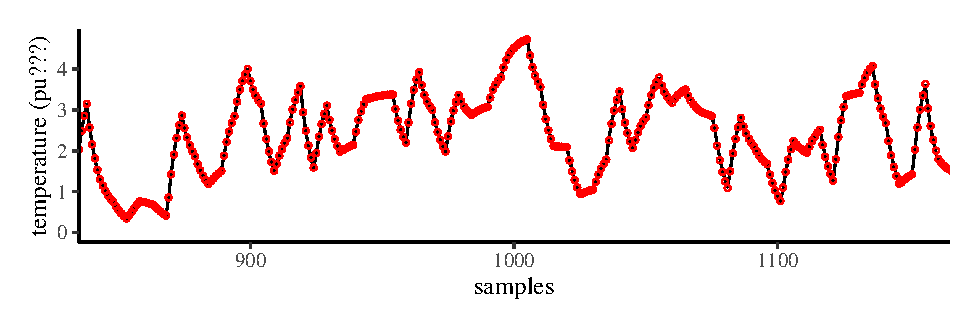
\includegraphics{./Figs/s.heater.var.dissip_train_val_data.eps}
    \caption{Resposta temporal para os dados de amostrados (preto tracejado -\ -), treinamento (círculos vermelhos $\color{red} \circ$), até a iteração 1000, e de validação (vermelho contínuo) a partir da milésima iteração. Para melhor visualização apenas as iterações de 850 a 1150 são mostradas. \todo[inline]{Corrigir axis labels} }
    \todo[color=orange, inline]{\textbf{LAA: } Não colocar dados de treinamento, somente validação. Deixar claro que foi utilizado free-run simulation.} 
    \label{fig:}
  \end{figure}

\end{exmp}



% \section{Control perfomance criteria}

% Como o objetivo deste trabalho é lidar com identificação e escolha de estruturas com o auxílio de estratégias VRFT, a serem aboradadas no capítulo \ref{cap:VRFT}, alguns conceitos necessários são apresentados nesta seção.
%
% Um elemento fundamental para projeto e análise de controladores na teoriade controle baseada em otimização, como é o caso do VRFT, é o conceito de \textit{desempenho de controle}. Na forma geral, este conceito pode ser expresso como a solução de um problema definido como
% \begin{equation}
%    \min_{\bm{\theta}} J(\bm{\theta}),
% \end{equation}
% onde $\vtheta \in \bm{R}$ é um vetor de $N$ parâmetros adotado como variável decisão e $J(\vtheta)$ é uma \textit{função de custo}\footnote{Outros termos também são conhecidos na literatura, como \textit{índice (ou função) de desempenho}, ou ainda, \textit{função objetivo}.}. Quanto menor o valor de $J$, melhor o desempenho segundo o critério adotado. Dependendo do objetivo de controle ou até mesmo por questões de garantias analíticas de estabilidade, diferentes funções de custo podem ser adotadas. Uma abordagem muito comum é escolher uma função de custo baseada na  norma-2 quadrática média\footnote{A norma-2 de um sinal discreto, ou vetor, $x(k)$ é definida como $||x(k)|| \triangleq \sqrt{ \sum_{k=1}^{N} [x(k)]^{2} }$. Elevando esse valor ao quadrado temos a norma-2 quadrática, que representa a energia do sinal que, dividida pelo número de amostras, como em \eqref{eq:H2}, resulta em sua energia média.}
% na forma
% \begin{equation}
%    ||x(k)||^{2} =\frac{1}{N}\sum_{k=1}^{N} \left[ x(k) \right]^{2} \triangleq \bar{\E} \left[ x(k) \right]^{2}
%    \label{eq:H2}
% \end{equation}
% em que $x(k)$ representa uma função genérica, $N$, o número de amostras e $\bar{\E}\left[ \cdot \right] $, um operador definido como
% \begin{equation}
%    \bar{\E}[x(k)] \triangleq \frac{1}{N}\sum_{k=1}^{N} [x(k)],
% \end{equation}
% que representa o cálculo da média amostral, e será usado no decorrer do texto em substituição ao somatório, por conveniência.
%
% O critério apresentado em \eqref{eq:H2} é conhecido como \textit{critério de desempenho} $H_2$ e é o que se adota neste trabalho e, para fins de objetividade, será o único abortado neste texto.
%
% O critério  $H_2$, para fins de controle, é definido de acordo com o objetivo de controle. Estes objetivos, em geral, são adotados como: (1) rastreamento de referência, (2) rejeição de ruídos e (3) economia de esforço de controle. Critérios mistos adotando mais de um destes objetivos, podem também ser definidos, como é o caso do (4) composite performance criteria. As próximas seções tratam destes critérios com um pouco mais de detalhes.

\section{Control System Setup and Notations}%
\label{sec:system_setup_}

Nesta seção apresenta-se o sistema em malha fechada considerado, definindo as equações para seus componentes e introduzindo a notação utilizada ao longo do texto. Como pretende-se lidar com sistemas não lineares, adota-se a notação apresentada em \cite{campi2006}. Quando lidando com sistemas lineares, porém, esta notação pode parecer mais pesada que o necessário e uma notação mais usual pode ser adotada. Essas notações, são apresentadas no escopo do sistema de controle considerado e são detalhadas nas próximas subseções.

\subsection{O sistema de controle}%
\label{sub:o_sistema_de_controle}

Considera-se um sistema de controle clássico do tipo SISO de um grau de liberdade, que pode ou não se encontrar sobre efeito de ruídos no sinal de saída. A figura \ref{fig:diagrama_MF} apresenta o diagrama de blocos deste sistema, onde $C(q, \bm{\theta}, e(k))$ representa o Controlador, função do vetor de parâmetros $\bm{\theta}$ e $P(q,u(k))$, o modelo do processo, ou planta, que pode ser ou não conhecido. Os sinais $r(k)$,
\todo{Corrigir aqui. Usar somente P e C no diagrama e corrigir neste parágrafo} 
$u(k)$, $\nu(t)$, $e(k)$, $y(k)$, e $y_\nu(k)$ são, respectivamente, os sinais de referência, controle, ruído, erro rastreamento, saída do processo e, por último, saída com ruído (ou sinal medido).

\begin{figure}[htpb] 
   \centering
   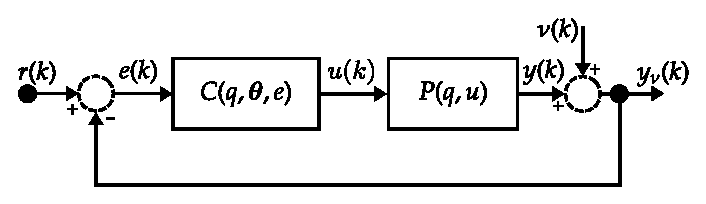
\includegraphics[width=0.8\textwidth]{Figs/diagrama_mf.eps}
   \caption{Sistema de controle.}
   \label{fig:diagrama_MF}
\end{figure}

\subsection{O Processo}%
\label{sub:o_processo}

O processo, ou planta, $P$ é um processo não-linear discreto no tempo do tipo SISO, com dinâmica não linear descrita como
\begin{equation}
   y(k)=p\left(y(k-1), \ldots, y(k-n_{P y}), u(k-1), \ldots, u(k-n_{P u})\right),
   \label{eq:yknl}
\end{equation}
onde $p$ é uma função representando o processo, $n_{P y}$ é o máximo atraso na saída, $n_{P u}$ é o máximo atraso na entrada e $k$ o índice temporal.

Por simplificação, é considerado que o atraso de tempo puro de $u$ para $y$ em $P$ é 1, mas o procedimento pode ser estendido sem problemas para atrasos maiores.

Considera-se $P$ como um mapa não-linear que opera de $\mathbb{R}^{N}$ para $\mathbb{R}^{N}$. Quando sujeito às condições iniciais $i.c.= (y(0), \ldots, y(1-n_{P y}), u(-1), \ldots, u(1-n_{P u}) )$ e a um sinal de entrada no intervalo $[0, N-1]$ definido como $u(0{:}N-1) \triangleq [u(0) \cdots u(N-1)]^{T}$, $P$ gera uma saída dada por
\begin{equation}
   y(1{:}N) = P[u(0{:}N-1), \text { i.c. }].
\label{eq:Pnl}
\end{equation}

Adota-se as seguintes hipóteses:
\begin{assum}\label{ass:psuave}
   A função $p$ que representa o processo é suave.
\end{assum}
\begin{assum}\label{ass:invert}
   Para quaisquer condições iniciais dadas, se $u_{1}(0{:}N-1) \neq u_{2}(0{:} N-1)$, então $P\left[u_{1}(0{:} N-1), i . c .\right] \neq P\left[u_{2}(0{:} N-1), i . c\right]$.
\end{assum}

A hipótese~\ref{ass:psuave} garante a invertibilidade do mapa $P$. A invertibilidade de $P$ para um sinal de entrada definido no intervalo $\left[ 0{:}N-1 \right]$
implica na invertibilidade do mapa em um intervalo $[0{:}T]$, com $T\le N-1$ \citep{campi2004}. \todo{Ref.\ aqui --olhar \citep{campi2006}.} 

\todo[inline]{Acabar aqui.} 

\subsection{O controlador}%
\label{sub:o_controlador}

O controlador considerado, assim como o processo, é representado por um modelo não-linear (que pode também ser linear). Para fins de identificação dos parâmetros pelo método VRFT, assunto abordado no capítulo \ref{cap:VRFT}, assume-se que uma estrutura (ou classe) é previamente escolhida. Este controlador pode ser descrito como
\begin{equation}
   u(k)=c\left(u(k-1), \ldots, u(k-n_{C u}), e(k), \ldots, e(k-n_{C e})\right),
\label{eq:uknl}
\end{equation}
em que $n_{Cu}$ e $n_{Ce}$ são os máximos atrasos no sinal de controle (saída do controlador e no sinal de erro de rastreamento (entrada do controlador).

Assim como para o processo, o controlador é sujeito às condições iniciais $i.c.= u(-1), \ldots, u(-n_{C u}), e(-1), \ldots, e(-n_{C e})$
e quando alimentado com o sinal de erro $e(0{:}N-1)$, gera o sinal de controle $u(0{:}N-1)$, que é representado por
\begin{equation}
   u(0{:}N-1)=C[e(0{:}N-1), i.c.].
\label{eq:Cnl}
\end{equation}

Neste trabalho, um dos objetivos é selecionar um controlador adequado dada uma classe fixa de controladores pelo método VRFT, conforme abordado no capítulo \ref{cap:VRFT}. Essa classe é formada por todos controladores parametrizados por
\begin{equation}
   u(k)=c\left(u(k-1), \ldots, u(k-n_{C u}), e(k), \ldots, e(k-n_{C e}); \bm{\theta}\right),
\label{eq:uknl_par}
\end{equation}
sendo $\bm{\theta} \in \mathbb{R}^{n_\theta}$ um vetor de $n_{\theta}$ parâmetros. O controlador parametrizado por $\bm{\theta}$ será aqui indicado por $C_{\theta}$, e o sinal de controle \eqref{eq:uknl} fica na forma 
\begin{equation}
   u_{\theta}(0{:}N-1)=C_{\theta}[e(0{:}N-1), i.c.],
\label{eq:utheta}
\end{equation}
com
\begin{equation}
   e(0{:} N-1)\triangleq r(0{:} N-1)-y(0{:} N-1)
\label{eq:erro}
\end{equation}
representando o erro de rastreamento.

A seguinte hipótese é assumida para o controlador:
\begin{assum}
   % O controlador $c(k)$ é uma função escalar \textit{suave} do vetor de parâmetros $\bm{\theta}$, de $u(k-1:k-n_{Cu})$  e de $e(k-0:k-n_{Ce})$, ou de forma simplificada
   O controlador $c$ é representado por uma função escalar parametrizada como em \eqref{eq:uknl_par}, e assumido suave, ou de forma simplificada
   \begin{equation}
      c:\mathbb{R}^{n_{Cu}+n_{Ce}+1+n_{\theta}} \mapsto \mathbb{R} \text{ é suave}.
      \label{eq:assumcon}
   \end{equation}
\end{assum}



\subsection{O Sistema Realimentado}%
\label{sub:o_sistema_realimentado}

As interconexões do sistema em malha fechada apresentado na figura \ref{fig:diagrama_MF}, juntamente com as equações do processo \eqref{eq:Pnl} e do controlador \eqref{eq:Cnl} resultam na relação
\begin{align}
   y(1: N) &=P[u(0{:} N-1), i . c .] \nonumber \\
   &=P[C[e(0{:} N-1), i . c .], i . c .]
   \label{eq:CLSnl}
\end{align}

\subsection{Simplificações nas notações}%
\label{sub:simplificações_nas_notações}

Por simplificações nas notações, considera-se as condições iniciais da planta e do controlador nulas. Tal requerimento não é necessário, porém só leva  a complicações desnecessárias, principalmente na notação. Além do mais, se as N é grande o suficiente, as condições iniciais influenciam pouco para casos estáveis.
Além disso, os argumentos temporais são omitidos, resultando no uso dos símbolos: $u$ para representar $u(0{:}N-1)$, $r$ para $r(0{:}N-1)$, $e$ para $e(0{:}N-1)$ e  $y$ para $r(1{:}N)$. Note o avanço temporal de $y$ em relação às outras variáveis. Desta forma, representa-se  $y(0{:}N)$ é representado por $Dy$, sendo $D$ uma matriz nilpotente de deslocamento em atraso definida como
\begin{equation}
   D \triangleq \begin{bmatrix} 
      0 & 0 & \dots & 0 & 0 \\
      1 & 0 & \dots & 0 & 0 \\
      0 & 1 & \dots & 0 & 0 \\
      \vdots & \vdots & \ddots & \vdots & \vdots \\
      0 & 0 & \dots & 1 & 0 \\
   \end{bmatrix} 
\label{eq:}
\end{equation}

Com isso, \eqref{eq:CLSnl} pode ser rescrita como
\begin{equation}
   y = P[C[r-Dy]]
   \label{eq:ymf}
\end{equation}
Ou, utilizando o controlador parametrizado de \eqref{eq:utheta},
\begin{equation}
   y_{\theta} = P[C_{\theta}[r-Dy_{\theta}]]
   \label{eq:ytheta}
\end{equation}


\subsection{The Control Objective}%
\label{sub:the_reference_model}

Um elemento fundamental para projeto e análise de controladores na teoriade controle baseada em otimização, como é o caso do VRFT, é o conceito de \textit{desempenho de controle}. Na forma geral, este conceito pode ser expresso como a solução de um problema definido como
\begin{equation}
   \min_{\bm{\theta}} J(\bm{\theta}),
\end{equation}
onde $\vtheta \in \mathbb{R}$ é um vetor de $n_{\theta}$ parâmetros adotado como variável decisão e $J(\bm{\theta})$ é uma \textit{função de custo}\footnote{Outros termos também são conhecidos na literatura, como \textit{índice (ou função) de desempenho}, ou ainda, \textit{função objetivo}.}. Quanto menor o valor de $J(\bm{\theta})$, melhor o desempenho segundo algum critério adotado. Dependendo do objetivo de controle, ou até mesmo por questões de garantias analíticas de estabilidade, diferentes funções de custo podem ser adotadas. Uma abordagem muito comum é escolher uma função de custo baseada na  norma-2 quadrática média\footnote{A norma-2 de um sinal discreto, ou vetor, $x(t)$ é definida como $||x(t)|| \triangleq \sqrt{ \sum_{t=1}^{N} [x(t)]^{2} }$. Elevando esse valor ao quadrado temos a norma-2 quadrática, que representa a energia do sinal que, dividida pelo número de amostras, como em \eqref{eq:H2}, resulta em sua energia média.}
na forma
\begin{equation}
   ||x(k)||^{2} =\frac{1}{N}\sum_{k=1}^{N} \left[ x(k) \right]^{2} \triangleq \bar{\E} \left[ x(k) \right]^{2}
   \label{eq:H2}
\end{equation}
em que $x(k)$ representa uma função genérica, $N$, o número de amostras e $\bar{\E}\left[ \cdot \right] $, um operador definido como
\begin{equation}
   \bar{\E}[x(k)] \triangleq \frac{1}{N}\sum_{k=1}^{N} [x(k)],
\end{equation}
que representa o cálculo da média amostral, e será usado no decorrer do texto em substituição ao somatório, por conveniência.

O critério apresentado em \eqref{eq:H2} é conhecido como \textit{critério de desempenho} $H_2$ e é o que se adota neste trabalho e, para fins de objetividade, será o único abortado neste texto.

O critério  $H_2$, para fins de controle, é definido de acordo com o objetivo de controle. Estes objetivos, em geral, são adotados como: (1) rastreamento de referência, (2) rejeição de ruídos e (3) economia de esforço de controle. Critérios mistos adotando mais de um destes objetivos, podem também ser definidos, como é o caso do (4) composite performance criteria. As próximas seções tratam destes critérios com um pouco mais de detalhes.


\subsubsection{The Reference Tracking Objective}%
\label{sub:the_reference_tracking_objective}
Um dos principais objetivos do controle em malha fechada é fazer com que o sinal controlado siga um sinal de referência desejado, de modo que sejam o mais próximo possível. Desprezando-se o efeito do ruído na saída, e considerando um controlador parametrizado, a resposta do sistema em malha fechada é dada por \eqref{eq:ytheta}.

Esse objetivo pode ser traduzido como a minimização de uma função custo dada pela norma-2 do erro de rastreamento, na forma
\begin{equation}
   % J(\bm{\theta}) = \bar{\E}\left[ r(t) - y_r(t,\bm{\theta}) \right].
   J_r(\bm{\theta}) \triangleq || r - y_\theta ||^2 .
   \label{eq:Jr}
\end{equation}
% onde o operador $\bar{\E}\left[ \cdot \right] $ (operador de média amostral), é definido como
% \begin{equation}
% \bar{\E}[\cdot] \triangleq \frac{1}{N}\sum_{k=1}^{N} [\cdot]^{2},
% \end{equation}
% e será usado no decorrer do texto em substituição ao somatório por conveniência.

\subsubsection{The Reference Model Objective}%
\label{sub:The Reference Model Objective}

Um fato bem conhecido na comunidade de controle é que na prática é impossível fazer com que a saída siga perfeitamente o sinal de referência durante todo o tempo, ou seja \eqref{eq:Jr} nunca será zero.
Para contornar esse fato uma saída é relaxar o objetivo de rastreamento por outro que satisfaça pré-requisitos desejados (como tempo de acomodação, instante de pico, sobressalto máximo, dentre outros), mas que seja menos exigente que a referência original.

Esse novo objetivo é traduzido para um modelo conhecido como \textit{modelo de referência} representado aqui por um mapa de $\mathbb{R}^{N}$ para $\mathbb{R}^{N}$, que mapeia um sinal de referência, digamos, $\tilde{r}$ para um sinal de saída $\tilde{y}$ com um comportamento desejado\footnote{o símbolo \ $\tilde{}$ \ enfatiza que estes sinais são para o modelo de referência.}.
\begin{equation}
   M:\tilde{r} \in \mathbb{R}^N \mapsto \tilde{y} \in \mathbb{R}^N
\label{eq:Mmap}
\end{equation}
Este mapa, a princípio pode ser um modelo não linear, desde que seja suave e invertível. Porém, em geral, por conveniência, é escolhido como um modelo linear, mas ainda sim deve ser invertível. Defini-se a seguinte hipótese:
\begin{assum}
   $M$ é triangular inferior e invertível.
\end{assum}
O fato de $M$ ser adotado como triangular inferior garante que será causal, com atraso puro maior ou igual a 1.
Um exemplo de escolha típica para $M$, para o caso linear, é o filtro
\begin{equation}
   M(q)=\frac{b_{1} q^{-1}+\cdots+b_{n_{M r}} q^{-n_{M r}}}{1+a_{1} q^{-1}+\cdots+a_{n_{M y}} q^{-n_{M y}}}
\label{eq:Mq}
\end{equation}
sendo $n_{Mr}$ e $n_{My}$ os máximos atrasos pra a referência e para a saída, respectivamente, e $q$ um operador de atraso. No domínio do tempo, \eqref{eq:Mq} corresponde a 
\begin{align}
   \label{eq:ytMr}
   \tilde{y}(k)=-a_{1} \tilde{y}(k-1)-\cdots &-a_{n_{M y}} \tilde{y}\left(k-n_{M y}\right) +b_{1} \tilde{r}(k-1)+\cdots+b_{n_{M r}} \tilde{r}\left(k-n_{M r}\right)
\end{align}

Uma vez definido o modelo de referência que traduz o comportamento desejado em malha fechada, o novo objetivo de controle é traduzido como

   % e será, neste texto, referido como $M(z)$, quando na forma de função de transferência (linear) ou $M(q)$ quando na forma de modelos temporais (linear ou não linear), ou simplesmente $M$ quando na forma apresentada na section \ref{sec:}. Neste sentido, uma nova função de custo é definida como
\begin{equation}
   J_y(\bm{\theta}) \triangleq \left\lVert y_\theta - \tilde{y} \right\lVert^{2} = \left\lVert P[C_\theta[\tilde{r}-Dy_\theta]] - M[\tilde{r}] \right\lVert^{2}
   % J_y(\bm{\theta}) \triangleq \bar{\E}\left[ y_r(k,\bm{\theta}) - y_{RM}(k) \right]^{2} = \bar{\E}\left[ T(q,\bm{\theta},r(k)) - M(q,r(k)) \right]^{2}
   \label{eq:Jy}
\end{equation}
sendo $\tilde{y} = M[\tilde{r}]$ o sinal de saída do modelo de referência desejado, quando sobre efeito de um sinal de referência $r$. Tal critério é conhecido como \textit{critério do modelo de referência}.


\subsubsection{The Noise Rejection Objective}%
\label{sub:the_noise_rejection_objective}

Outro objetivo comum em sistemas de controle é minimizar o efeito do ruído no sinal de saída. O sinal de saída devido somente a atuação do sinal de ruído no processo pode ser escrito como
\begin{equation}
   y_{\theta\nu}(\bm{\theta}) \triangleq S_\theta[\nu] = \nu-P[C_\theta[Dy_{\theta\nu}],
\end{equation}
em que $\nu \triangleq \nu(0{:}N)$ representa o sinal de ruído e $S_{\theta}$ um mapa de ruído para a saída do processo, ou seja $M:\nu \mapsto y_{\theta\nu}$, que, para o caso linear, é também conhecido como função sensibilidade. Quando analisada a magnitude deste sinal em função de alguma norma, tem-se o critério de desempenho de rejeição de ruído $J_\nu(\bm{\theta})$ que, utilizando a norma-2, é dado por
\begin{equation}
   J_\nu(\bm{\theta}) \triangleq \norm{ y_{\theta\nu} }^2 = \norm{ S_\theta[\nu] }^2.
   \label{eq:Jnoise}
\end{equation}.

Assim como no caso do rastreamento, não é possível a eliminação completa do efeito do ruído e um relaxamento neste critério é desejável, pelos mesmos motivos. Neste caso é definida uma função sensibilidade desejada $S_{M}$\footnote{O índice $M$ é utilizado para manter a analogia com o índice utilizado pelo modelo de referência para o caso de rastreamento.} e adota-se o critério
\begin{equation}
   J_\nu^{M}(\bm{\theta}) \triangleq  \norm{S_\theta[\nu] - S_M[\nu]}^{2}.
   \label{eq:JeRM}
\end{equation}





\subsubsection{The Economy of Control Effort Objective}%
\label{sub:the_economy_of_control_effot_objective}

Um objetivo comum no projeto de controladores, principalmente na área de controle ótimo, é a minimização do esforço de controle. Para minimizar o sinal de controle o seguinte índice pode ser definido:
\begin{equation}
   J_u(\bm{\theta}) \triangleq \norm{ u(k) }^{2},
   \label{eq:Ju}
\end{equation}
sendo $u(k)$ o sinal de controle. Porém este índice não deve ser usado sozinho, uma vez que $J_u(\bm{\theta}) = 0$ implicaria em $u \equiv 0$. Portanto o que se faz é utilizar-se de uma combinação deste índice, com outros, por exemplo, com o objetivo de rastreamento de referência, resultando em 
\begin{equation}
   J_\lambda = J_y(\bm{\theta}) + \lambda J_u(\bm{\theta})
   \label{eq:Jl}
\end{equation}
em que $\lambda \in \mathbb{R}$ representa um parâmetro de ajuste.
Ao se utilizar de controladores baseados em modelo de referência, como o caso do VRFT a ser visto no \ref{cap:VRFT}, um efeito de economia de esforço de controle pode ser obtido ao se escolher um modelo de referência adequado. Portanto, neste trabalho a inclusão do índice \eqref{eq:Ju} na função de custo é desconsiderado.



\subsubsection{The Composite Performance Objective}%
\label{sub:the_composite_performance_objective}

Outro objetivo, mais realista que o de rastreamento de referência, é o \textit{composite performance}, que objetiva tanto reduzir o erro de rastreamento quanto rejeitar efeitos do ruído na saída. Este critério é dado por
\begin{equation}
   J_T(\bm{\theta}) \triangleq \norm{ y_{\theta\nu} - \tilde{y} }^2,
   \label{eq:JT}
\end{equation}
em que, diferentemente de $\tilde{y}$ em \eqref{eq:Jy}, o sinal $y_{\theta\nu}= P[C_\theta[r-y_\theta]] + S[\nu]$ depende do ruído. O critério final será a soma dos dois critérios anteriores, uma vez que a referência e o ruído são sinais independentes estatisticamente e pode ser escrito como

\begin{equation}
   J_T(\bm{\theta}) = \norm{ P[C_\theta[r-Dy_\theta]] - M[r] }^{2} + \norm{ S[\nu] }^2.
   \label{eq:}
\end{equation}






\section{The Ideal Controller and the Matched Control}%
\label{sub:the_ideal_controller_and_the_matched_control}
\todo{Tirar o ``Matched Control??''.}

Considerando o sistema realimentado apresentado em \eqref{eq:ymf}, e assumindo a invertibilidade de $P$ e que $M$ é triangular inferior, resolvendo \eqref{eq:ymf} para $C$, é possível calcular o controlador ideal, que resulta nos parâmetros ótimos para $C_\theta$, desde que $C_\theta$ tenha mesma estrutura (ou pertença à mesma classe) do controlador ideal. Este controlador ideal é definido como:
\begin{equation}
   C_0 \triangleq P^{-1}(I-MD)^{-1}M,
\label{eq:}
\end{equation}
onde $I$ é a matriz identidade e $C^{i}$ é o controlador ideal.

Quando o $C_0$ é usado na malha fechada, o mapa de $r$ para $y$ é dado por $M$, ou seja, $y=M[r]$

Para o caso linear SISO (Single Input Single Output), se o modelo do processo é conhecido e considerando que este é de 
% \todo{[DONE] Falar aqui (citar) do trabalho da Lucíola no sentido de lidar com fase não mínima. Talvez citar Stogestad também.}
fase mínima, o controlador ideal $C_0$ pode ser escrito na forma de função de transferência como
\begin{equation}
   C_0(z) = \frac{M(z)}{P(z)\left(1-M(z)\right)},
   \label{eq:Cdz}
\end{equation}
em que $P(z)$ e $M(z)$ representam respectivamente as funções de transferência do processo e do modelo de referência.

Note que, se o processo é de fase não mínima, devido a zeros fora do círculo unitário no plano-$z$, a inversa de $P(z)$ em \eqref{eq:Cdz} resulta em instabilidade do sistema. Soluções para este problema têm sido apresentadas há décadas para projetos MBC, como por exemplo regras para sintonia de PID, como a desenvolvida por \cite{skogestad2003}.
Uma abordagem no mais recente, no âmbito do DDC, é apresentada por \cite{campestrini2011}.
\todo{Colocar um pouco mais sobre esteartigo aqui.} 


\todo[inline]{Colocar aqui a respeito do caso não linear, como em \cite[p. 19]{campi2006}, mas antes introduzir notação.}






\clearpage
\thispagestyle{empty}
\cleardoublepage
% }}} ------------------------------------------------------------------

% % {{{ Captulo 3 - VRFT
 % -*- TeX-master: "Qualificacao.tex" -*-
%!TEX root = Qualificacao.tex
\chapter{Virtual Reference Feedback Tuning}\label{cap:VRFT}
\vspace{-1cm}

% \section{Introdução}\label{sec:introvrft}

% O método \emph{Virtual Reference Feedback Tunning}, ou simplesmente VRFT, é um procedimento que visa o projeto de controladores realimentados a partir somente de dados amostrados do processo, sem a necessidade de um modelo que descreva este último. Com isso, se classifica como um método de controle baseado em dados, ou DDC.

The \textit{Virtual Reference Feedback Tunning} method, or simply VRFT, proposed by \cite{campi2002}, is a procedure that aims to design closed loop controllers based only on data sampled from the process, without the need for a model that describes that process itself. Thus, it is classified as a data-based control method, or DDC.

% O principal objetivo deste método é ajustar os parâmetros de um controlador, definido por uma função paramétrica, a partir de dados amostrados do processo, a fim de que o sinal de saída do processo controlado tenha um comportamento o mais próximo possível do sinal de saída de um modelo de referência previamente definido.
The main objective of this method is to adjust the parameters of a controller, defined by a parametric function like \eqref{eq:uknl_par}, using the process sampled data only, so that the output signal of the controlled process, $y_\theta(k)$ behaves as close as possible to the output signal $\tilde{y}$ of a previously defined reference model as defined in \eqref{eq:Mmap}.
To reach this objective, VRFT aims to optimize the tracking error by minimizing a performance index $J_y(\vtheta)$ as stated in \eqref{eq:Jy}, rewritten here for convenience:
\begin{equation}
   J^N_y(\bm{\theta}) \triangleq \lim_{N \to \infty}  \frac{1}{N} \sum_{k=1}^N \left[y(k,\vtheta) - \hat{y}(k)\right]^2 = 
    \left\lVert y_\theta - \tilde{y} \right\lVert^{2}
   \label{eq:Jy},
\end{equation}
% sendo $N$ o número de dados amostrados,  $\vtheta = \begin{bmatrix} \theta_1 & \theta_2 & \cdots & \theta_N \end{bmatrix}^T \in \R^n$ um vetor de parâmetros, $k$ um índice temporal
% % , $\E[\cdot]$ um operador que representa o cálculo da esperança
% com $y_r(k,\vtheta)$ e $y_{MR}(k)$, definidos como se segue:
where $N$ represents the number of data samples, $\vtheta = \begin{bmatrix} \theta_1 & \theta_2 & \cdots & \theta_N \end{bmatrix}^T \in \R^N$ a vector of parameters and $k$ a temporal index. The signal $y_\theta(k) \in \R $ represents the output of the  system controlled with the parametrized controller $C_\theta$, and $\tilde{y}(k) \in \mathbb{R}$ are the output of a reference model $M$, both subject to the same reference signal.

% \begin{itemize}
   % % \item $y_r(k,\vtheta)$ representa a resposta obtida em malha fechada utilizando um controlador com parâmetros $\vtheta$, quando sobre o efeito de um sinal de referência $r(k)$, ou seja
   % \item $y_{r}(k)$ represents the response obtained in closed loop using a controller with  parameters $\vtheta$, when under the effect of a  reference signal $r(k)$, i.e.
      % \begin{equation}
         % y_r(k,\vtheta) \triangleq M(q,\vtheta)r(k)
         % \label{eq:yr},
      % \end{equation}
      % % onde $M(q,\vtheta)$ representa o modelo em malha fechada do sistema controlado, função do vetor de parâmetros $\vtheta$ e $q$ um operador de deslocamento temporal.
      % where $M(q,\vtheta)$ represents the closed loop model of the controlled system, function of the vector of parameters, $\vtheta$, and a time displacement operator, $q$.
      % % \item $y_{mr}(k)$ representa a resposta temporal obtida ao se aplicar o sinal de referência $r(k)$ como sinal de entrada de um modelo $M(q)$, conhecido como \textit{modelo de referência} e que representa o comportamento desejado em malha fechada, ou seja
   % \item $y_{MR}(k)$ represents the temporal response obtained by applying the reference signal $r(k)$ as an input signal for a model $M(q)$, known as a \textit{reference model} and representing the desired closed-loop behavior, i.e.
      % \begin{equation}
         % y_{MR}(k) \triangleq M(q)r(k)
         % \label{eq:yMR},
      % \end{equation}
% \end{itemize}

% Para alcançar o objetivo de minimizar \eqref{eq:Jy}, \cite{campi2002}, para o caso linear, e \cite{campi2006}, para o caso não linear, mostram que, sob certas condições, apresentadas na sequência, ao se minimizar um índice de custo definido como
To achieve the objective of minimizing \eqref{eq:Jy}, \cite{campi2002}, for the linear case, and \cite{campi2006}, for the non-linear case, show that, under certain conditions, presented in sequence, when minimizing a cost index defined as
\begin{equation}
   J_{VR}(\vtheta) \triangleq \lim_{N \to \infty}  \frac{1}{N} \sum_{k=1}^N \left[u(k) - C_\theta(q,\vtheta)\bar{e}(k)\right]^2
   \label{eq:Jvr},
\end{equation}
% minimiza-se também o índice $J_y(\theta)$ definido em ~\eqref{eq:Jy}. Em \eqref{eq:Jvr}, $u(k)$ representa o sinal de entrada aplicado ao processo durante a coleta de dados, $C(q,\vtheta)$ o modelo do controlador a ser ajustado e $e(k)$ é o chamado \textit{erro virtual}, definido como
the index $J_y(\vtheta)$ defined in~\eqref{eq:Jy} is also minimized. In~\eqref{eq:Jvr}, $u(k)$ represents the input signal applied to the process during data collection, $C (q,\vtheta)$ the controller model to be adjusted and $\bar{e}(k)$ is the so-called \textit{virtual error}, defined as
\begin{equation}
   \ev(k) = \rv(k) - y(k) 
   \label{eq:ev},
\end{equation}
% onde $\rv$ é o sinal de \textit{referência virtual}, obtido ao se filtrar a saída $y(k)$ pelo modelo de referência inverso, na forma
where $\rv$ is a signal called \textit{virtual reference}, obtained by filtering the output $y(k)$ by the inverse reference model $M^{-1}(q)$, in the form
\begin{equation}
   \rv(k) = M^{-1}(q)y(k)
   \label{eq:refvirt}.
\end{equation}

% O termo ``virtual'' é adotado nos sinais de referência e erro para enfatizar que nenhum destes sinais são fisicamente disponíveis, mas apenas calculados para fins de projeto do controlador. \todo{melhorar isso aqui.}
The term ``virtual'' is adopted in reference tracking error signals to emphasize that none of these signals are physically available, but only calculated for controller design purposes, as will be better explained latter. \todo{improve this here.}

% Como mencionado anteriormente, para que $J_y(\vtheta)$ e  $J_{VR}(\vtheta)$ apresentem seus valores mínimos para a mesma solução de parâmetros $\vtheta$, certas condições devem ser satisfeitas. Estas condições são apresentadas na sequência, logo após algumas definições que se mostram importantes para o restante do capítulo.
The condition for  $J_y(\vtheta)$ and $J_{VR}(\vtheta)$ reach their minimum values for the same parameter solution $\vtheta$ are presented in sequence, right after some definitions that are important for the rest of the chapter.

\section{Basic definitions}\label{sec:vrft_basic_def}

\begin{defn}[Ideal Controller]\label{def:idealControler}
   \todo[inline]{Put definition here.}
\end{defn}

\begin{assum}[Noise free]\label{ass:noiseFree} 
   The system is not affected by noise.
\end{assum}

\begin{assum}[Matched control]\label{ass:machedControl} %% Assumption By of \citep{bazanella2012} pg 13 
   The ideal controller belongs to control model class considered, i.e. $C_0(q) \in \mathscr{C}$, or, equivalently
   \begin{equation}
      \exists \bm{\theta}_0 : C(q,\bm{\theta}_0)=C_0(q)
      \label{eq:assumpMatched}.
   \end{equation}
\end{assum}

\begin{figure}[H]
   \centering
   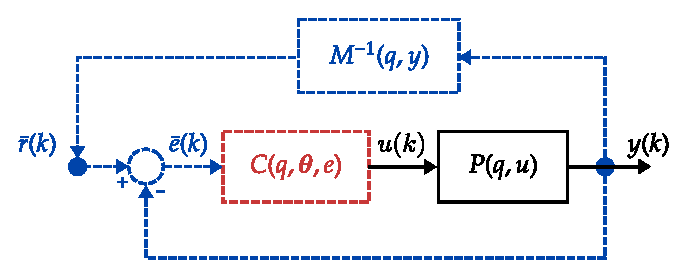
\includegraphics{Figs/diagrama_VRFT.eps}
   \caption{ Experiment to obtain the data used to identify the controller parameters by the VRFT method:
   real data (\textit{black solid lines}), virtual data (\textit{blue dashed lines}) and the cotroller to tune in (\textit{red dashed block}).}
   \label{fig:Figs-diagrama_VRFT-eps}
\end{figure}

\section{Filtro Caso não Linear}%
\label{sec:filtro_caso_não_linear}

Objetivo do filtro
\begin{equation}
   J_{\mathrm{VRFT}}\left(\theta^{+}\right):=\left\|F\left[C_{\theta}+[\tilde{e}]\right]-F[\tilde{u}]\right\|^{2}
   \label{eq:JVR}
\end{equation}
Deseja-se selecionar um filtro tal que \begin{equation}
   \left.\frac{\partial^{2} J_{\mathrm{VRFT}}\left(\theta^{+}\right)}{\partial \theta^{+2}}\right|_{\theta_{0}^{+}}=\left.\frac{\partial^{2} J\left(\theta^{+}\right)}{\partial \theta^{+2}}\right|_{\theta_{0}^{+}}
   \label{eq:condToF}
\end{equation}

\begin{theorem}
   Se 
   \begin{equation}
       F=(I-M D)\left(\left.\frac{\partial P[u]}{\partial u}\right|_{\tilde{u}}\right)
       \label{eq:FiltroVRFTNL}
   \end{equation}
   então \eqref{eq:condToF} é satisfeita.
\end{theorem}


\section{Prova da escolha do filtro VRFT}%
\label{sec:prova_da_escolha_do_filtro_vrft}
Note que
\begin{equation}
\tilde{u}=C_{\theta_{0}^{+}}[\tilde{e}]
\label{eq:uTil}
\end{equation}
uma vez que
\begin{align}
   \tilde{u}&=P^{-1}[\hat{y}]=P^{-1}\left[(I-M D)^{-1}(I-M D) \hat{y}\right] \nonumber\\
            &= P^{-1}\left[(I-M D)^{-1}(M \tilde{r}-M D \tilde{y})\right]=P^{-1}\left[(I-M D)^{-1} M \tilde{e}\right] = C^{0}[\tilde{e}] \nonumber\\
            &=C_{\theta_{0}^{+}}[\tilde{e}].
\end{align}

De forma semelhante
\begin{equation}
   \tilde{y}=y_{\theta_{0}^{+}}
\label{eq:yqp}
\end{equation}
uma vez que, $\tilde{y}=P[\tilde{u}]$ a partir de \eqref{eq:uTil}, assumindo $\tilde{e}=\tilde{r}-D \tilde{y}$,  tem-se que $\tilde{y}=P\left[C_{\theta_{0}^{+}}[\tilde{e}]\right]=$$P\left[C_{\theta_{0}^{+}}[\tilde{r}-D \tilde{y}]\right]$. Como
$y_{\theta_{0}^{+}}=P\left[C_{\theta_{0}^{+}}\left[\tilde{\tilde{r}}-D y_{\theta_{0}^{+}}\right]\right]$, 
$\tilde{y}$ e $y_{\theta_{0}^{+}}$ corresponde ao mesmo $\tilde{r}$ no mapa $r \mapsto y$ dado por $y=P\left[C_{\theta_{0}^{+}}[r-D y]\right]$.
% $\tilde{y}$ e $y_{\theta_{0}^{+}}$ corresponde ao mesmo $\tilde{r}$ in the $r$ to $y$ map given by $y=P\left[C_{\theta_{0}^{+}}[r-D y]\right]$
Uma vez que tal mapa, dado um $r$ há somente um $y$ correspondente, conclui-se \eqref{eq:yqp}.
De \eqref{eq:yqp} é possível concluir que 
\begin{equation}
   \tilde{r}-D y_{\theta_{0}^{+}}=\tilde{e},
\label{eq:eTil}
\end{equation}
que, em \eqref{eq:uTil}, resulta em
\begin{equation}
\tilde{u}=C_{\theta_{0}^{+}}\left[\tilde{r}-D y_{\theta_{0}^{+}}\right].
\label{eq:uTil_2}
\end{equation}

% Parei aqui...

Por simplicidade e maior clareza no desenvolvimento, adota-se a seguinte notação:
\begin{align}
   x_{\theta^{+}} &\triangleq F\left[C_{\theta^{+}}[\tilde{e}]\right]-F[\tilde{u}] \label{eq:x} \\
   w_{\theta^{+}} &\triangleq y_{\theta^{+}}-\tilde{y} \label{eq:w} \\
   \frac{\partial g}{\partial \theta^{+}} &\triangleq 
   \begin{bmatrix} 
      \partial g_1/\partial \theta^{+}_1 & \dots & \partial g_1/\partial \theta^{+}_j & \dots & \partial g_1/\partial \theta^{+}_{n_{\theta +}} \\
      \vdots &  & \vdots & & \vdots \\
      \partial g_i/\partial \theta^{+}_1 & \dots & \partial g_i/\partial \theta^{+}_j & \dots & \partial g_i/\partial \theta^{+}_{n_{\theta +}} \\
      \vdots & & \vdots & & \vdots \\
      \partial g_N/\partial \theta^{+}_1 & \dots & \partial g_N/\partial \theta^{+}_j & \dots & \partial g_N/\partial \theta^{+}_{n_{\theta +}}
   \end{bmatrix} \label{eq:partg}
\end{align}
   % \partial g /\partial \theta^{+} &\triangleq \partial g(i)  /\partial \theta^{+}_j \label{eq:partg}
\todo{Olhar \eqref{eq:partg}. Não é bem isso, na verdade é uma matriz.} 
Sendo \eqref{eq:partg} (em que $g$ é uma função genérica) definida tal que o $(i,j)$-ésimo elemento é $\partial g(i)  /\partial \theta^{+}_j$, de modo que as colunas $(j)$ correspondem às derivadas de $g$ em relação a diferentes parâmetros e as linhas $(i)$ correspondem à evolução temporal.

Usando \eqref{eq:x} e \eqref{eq:w}, as função de custo \eqref{eq:JVR} e \eqref{eq:Jy} são rescritas como
$$
J_{\mathrm{VR}}\left(\theta^{+}\right)=\left\|x_{\theta^{+}}\right\|^{2} \qquad J\left(\theta^{+}\right)=\left\|w_{\theta^{+}}\right\|^{2}
$$
Calculando a primeira e segunda derivadas de $J_{\mathrm{VR}}\left(\theta^{+}\right)$ com respeito ao vetor de parâmetros $\theta^+$, para aproximação por séries de Taylor:
\begin{align}
   \frac{\partial J_{\mathrm{VR}}\left(\theta^{+}\right)}{\partial \theta^{+}} &=\frac{\partial x_{\theta^{+}}^{T} x_{\theta^{+}}}{\partial \theta^{+}} = 2 x_{\theta^{+}}^{T}\left(\frac{\partial x_{\theta^{+}}}{\partial \theta^{+}}\right), \\
\frac{\partial^{2} J_{\mathrm{VR}}\left(\theta^{+}\right)}{\partial \theta^{+2}}&= 2 x_{\theta^{+}}^{T}\left(\frac{\partial^{2} x_{\theta^{+}}}{\partial \theta^{+2}}\right)
+2\left(\frac{\partial x_{\theta^{+}}}{\partial \theta^{+}}\right)^{T}\left(\frac{\partial x_{\theta^{+}}}{\partial \theta^{+}}\right). 
\end{align}
Utilizando \eqref{eq:x} e \eqref{eq:uTil} e calculando as derivadas para o ponto de equilíbrio $\theta^{+}_0$, resulta em
\begin{align}
\left.J_{\mathrm{VR}}\left(\theta^{+}\right)\right|_{\theta_{0}^{+}}
& =\left.\frac{\partial J_{\mathrm{VR}}\left(\theta^{+}\right)}{\partial \theta^{+}}\right|_{\theta_{0}^{+}} =0 \label{eq:JVRTaylor_1}\\
   \left.\frac{\partial^{2} J_{\mathrm{VRFT}}\left(\theta^{+}\right)}{\partial \theta^{+2}}\right|_{\theta_{0}^{+}} &= 2\left(\left.\frac{\partial x_{\theta^{+}}}{\partial \theta^{+}}\right|_{\theta_{0}^{+}}\right)^{T}\left(\left.\frac{\partial x_{\theta^{+}}}{\partial \theta^{+}}\right|_{\theta_{0}^{+}}\right) \label{eq:JVRTaylor_2}
\end{align}

Fazendo o mesmo procedimento para $J\left(\theta^{+}\right)=\left\|w_{\theta^{+}}\right\|^{2}$:
\begin{align}
\frac{\partial J\left(\theta^{+}\right)}{\partial \theta^{+}} 
   &=\frac{\partial w_{\theta^{+}}^{T} w_{\theta^{+}}}{\partial \theta^{+}}=2 w_{\theta^{+}}^{T}\left(\frac{\partial w_{\theta^{+}}}{\partial \theta^{+}}\right), \\
\frac{\partial^{2} J\left(\theta^{+}\right)}{\partial \theta^{+2}}&= 2 x_{\theta^{+}}^{T}\left(\frac{\partial^{2} w_{\theta^{+}}}{\partial \theta^{+2}}\right) 
+2\left(\frac{\partial w_{\theta^{+}}}{\partial \theta^{+}}\right)^{T}\left(\frac{\partial w_{\theta^{+}}}{\partial \theta^{+}}\right).
\label{eq:}
\end{align}
Usando \eqref{eq:w} e \eqref{eq:yqp}:
\begin{align}
\left.J\left(\theta^{+}\right)\right|_{\theta_{0}^{+}}                                                                      
&=\left.\frac{\partial J\left(\theta^{+}\right)}{\partial \theta^{+}}\right|_{\theta_{0}^{+}}=0 \label{eq:JyTaylor_1} \\
   \left.\frac{\partial^{2} J\left(\theta^{+}\right)}{\partial \theta^{+2}}\right|_{\theta_{0}^{+}} &= 2\left(\left.\frac{\partial w_{\theta^{+}}}{\partial \theta^{+}}\right|_{\theta_{0}^{+}}\right)^{T}\left(\left.\frac{\partial w_{\theta^{+}}}{\partial \theta^{+}}\right|_{\theta_{0}^{+}}\right) . \label{eq:JyTaylor_2}
\end{align}

Somando os termos de \eqref{eq:JVRTaylor_1} a \eqref{eq:JVRTaylor_2}, e os \eqref{eq:JyTaylor_1} e \eqref{eq:JyTaylor_2}, tem-se, respectivamente uma aproximação de segunda ordem por séries de Taylor. E para que o objetivo do filtro \eqref{eq:FiltroVRFTNL} seja alcançado, ou seja $ J_{\mathrm{VR}}\left(\theta^{+}\right) \approx J\left(\theta^{+}\right)$, comparando \eqref{eq:JVRTaylor_2} com \eqref{eq:JyTaylor_2}, deve-se ter  
\begin{equation}
   \left.\frac{\partial x_{\theta^{+}}}{\partial \theta^{+}}\right|_{\theta_{0}^{+}}=\left.\frac{\partial w_{\theta^{+}}}{\partial \theta^{+}}\right|_{\theta_{0}^{+}}
   \label{eq:FilterObjective}
\end{equation}

Usando a notação 

\begin{equation}
   \frac{\partial P[u]}{\partial u} \triangleq 
   \begin{bmatrix} 
      \partial P[u]_1/\partial u_0 & \dots & \partial P[u]_1/\partial u_{(j-1)} & \dots & \partial P[u]_1/\partial u_{(N-1)} \\
      \vdots &  & \vdots & & \vdots \\ 
      \partial P[u]_i/\partial u_0 & \dots & \partial P[u]_i/\partial u_{(j-1)} & \dots & \partial P[u]_i/\partial u_{(N-1)} \\
      \vdots & & \vdots & & \vdots \\ 
      \partial P[u]_N/\partial u_0 & \dots & \partial P[u]_N/\partial u_{(j-1)} & \dots & \partial P[u]_N/\partial u_{(N-1)}
   \end{bmatrix}  
   \label{eq:PuDu}
\end{equation}
e resolvendo o lado esquerdo de \eqref{eq:FilterObjective}, considerando que o filtro $F$ é linear, chega-se a
\begin{equation}
   \left.\frac{\partial x_{\theta^{+}}}{\partial \theta^{+}}\right|_{\theta_{0}^{+}}=\left.\frac{\partial F\left[C_{\theta^{+}}[\tilde{e}]\right]}{\partial \theta^{+}}\right|_{\theta_{0}^{+}}=F\left(\left.\frac{\partial C_{\theta^{+}}[\tilde{e}]}{\partial \theta^{+}}\right|_{\theta_{0}^{+}}\right)
\label{eq:28}
\end{equation}

Como $C_{\theta_0^+} = \tilde{u}$, ver \eqref{eq:uTil}, o lado direito de \eqref{eq:FilterObjective} é calculado como
\begin{align}
\left.\left.\frac{\partial P[u]}{\partial u}\right|_{\tilde{u}} \frac{\partial C_{\theta_{0}^{+}}[e]}{\partial e}\right|_{\tilde{e}} &=\left.\frac{\partial P\left[C_{\theta_{0}^{+}}[e]\right]}{\partial e}\right|_{\tilde{e}} \nonumber\\
&=\left.\frac{\partial(I-M D)^{-1} M[e]}{\partial e}\right|_{\tilde{e}} \nonumber\\
&=(I-M D)^{-1} M .
\label{eq:29}
\end{align}

Aplicando a regra da cadeia, em $(\partial y_{\theta_0^+}/\partial \theta^+)$:
\begin{align}
\left.\frac{\partial y_{\theta^{+}}}{\partial \theta^{+}}\right|_{\theta_{0}^{+}}=&\left.\frac{\partial P\left[C_{\theta^{+}}\left[\tilde{r}-D y_{\theta^{+}}\right]\right]}{\partial \theta^{+}}\right|_{\theta_{0}^{+}} \\
=&\left.\frac{\partial P[u]}{\partial u}\right|_{C_{\theta_{0}^{+}}\left[\tilde{r}-D y_{\theta_{0}^{+}}\right]} 
   \left\{\left.\left.\frac{\partial C_{\theta^{+}}\left[\tilde{r}-D y_{\theta_{0}^{+}}\right]}{\partial \theta^{+}}\right|_{\theta_{0}^{+}}{-\left.\frac{\partial C_{\theta_{0}^{+}}[e]}{\partial e}\right|_{\tilde{r}-D y_{\theta_{0}^{+}}}} \frac{\partial D y_{\theta^{+}}}{\partial \theta^{+}}\right|_{\theta_{0}^{+}}\right\}
\end{align}
%
Usando \eqref{eq:eTil} e \eqref{eq:uTil_2},
\begin{equation}
   \left.\frac{\partial y_{\theta^{+}}}{\partial \theta^{+}}\right|_{\theta_{0}^{+}}=\left.\frac{\partial P[u]}{\partial u}\right|_{\tilde{u}}\left\{\left.\frac{\partial C_{\theta^{+}}[\tilde{e}]}{\partial \theta^{+}}\right|_{\theta_{0}^{+}}\right.
   \left.-\left.\left.\frac{\partial C_{\theta_{0}^{+}}[e]}{\partial e}\right|_{\tilde{e}} \frac{\partial D y_{\theta^{+}}}{\partial \theta^{+}}\right|_{\theta_{0}^{+}}\right\}
\end{equation}


e então
\begin{equation}
   \left.\left.\frac{\partial P[u]}{\partial u}\right|_{\tilde{u}} \frac{\partial C_{\theta^{+}}[\tilde{e}]}{\partial \theta^{+}}\right|_{\theta_{0}^{+}}
   =
   \left.\frac{\partial y_{\theta^{+}}}{\partial \theta^{+}}\right|_{\theta_{0}^{+}}+\left.\left.\left.\frac{\partial P[u]}{\partial u}\right|_{\tilde{u}} \frac{\partial C_{\theta_{0}^{+}}[e]}{\partial e}\right|_{\tilde{e}} \frac{\partial D y_{\theta^{+}}}{\partial \theta^{+}}\right|_{\theta_{0}^{+}}.
\end{equation}

Substituindo em \eqref{eq:29} resulta em
\begin{equation}
   \left.\frac{\partial y_{\theta^{+}}}{\partial \theta^{+}}\right|_{\theta_{0}^{+}}+(I-M D)^{-1} M \frac{\partial D y_{\theta^{+}}}{\partial \theta^{+}} \left.\right|_{\theta_{0}^{+}}
   =\left.\left.\frac{\partial P[u]}{\partial u}\right|_{\tilde{u}} \frac{\partial C_{\theta^{+}}[\tilde{e}]}{\partial \theta^{+}}\right|_{\theta_{0}^{+}},
\end{equation}
que, multiplicando por $(I-MD)$, nos dá
\begin{equation}
   \left.\frac{\partial y_{\theta^{+}}}{\partial \theta^{+}}\right|_{\theta_{0}^{+}}-\left.M D \frac{\partial y_{\theta^{+}}}{\partial \theta^{+}}\right|_{\theta_{0}^{+}}+\left.M \frac{\partial D y_{\theta^{+}}}{\partial \theta^{+}}\right|_{\theta_{0}^{+}}
   =\left.\left.(I-M D) \frac{\partial P[u]}{\partial u}\right|_{\tilde{u}} \frac{\partial C_{\theta^{+}}[\tilde{e}]}{\partial \theta^{+}}\right|_{\theta_{0}^{+}}
\end{equation}
Por fim, o termo do lado direito de \eqref{eq:FilterObjective}, pode ser escrito como
\begin{equation}
   \left.\frac{\partial w_{\theta^{+}}}{\partial \theta^{+}}\right|_{\theta_{0}^{+}} =\left.\frac{\partial y_{\theta^{+}}}{\partial \theta^{+}}\right|_{\theta_{0}^{+}} 
   =\left.\left.(I-M D) \frac{\partial P[u]}{\partial u}\right|_{\tilde{u}} \frac{\partial C_{\theta^{+}}[\tilde{e}]}{\partial \theta^{+}}\right|_{\theta_{0}^{+}}
\end{equation}
que, comparando com \eqref{eq:28}, conclui-se que
\begin{equation}
   F=(I-M D)\left(\left.\frac{\partial P[u]}{\partial u}\right|_{\tilde{u}}\right) .
\label{eq:FiltroFinal}
\end{equation}



 \clearpage
 \thispagestyle{empty}
 \cleardoublepage
% % }}} ------------------------------------------------------------------

% {{{ Captulo 4 - Reinforcement Learning

% -*- TeX-master: "Qualificacao.tex" -*-
%!TEX root = Qualificacao.tex
\chapter{Reinforcement Learning}\label{cap:RL}
\vspace{-1cm}

% Frase citação inicial {{{1
% \begin{flushright}
% \begin{minipage}{0.7\linewidth}
%     \emph{``\dots''}
% \end{minipage}
% \end{flushright}
%
% \begin{flushright}
% Cicrano
% \end{flushright}
%
%\vspace{1cm}

O Capítulo de RL vai aqui.


% % -*- TeX-master: "Qualificacao.tex" -*-
%!TEX root = Qualificacao.tex
\chapter{Reinforcement Learning}\label{cap:RL}
\vspace{-1cm}

% Frase citação inicial {{{1
% \begin{flushright}
% \begin{minipage}{0.7\linewidth}
%     \emph{``\dots''}
% \end{minipage}
% \end{flushright}
%
% \begin{flushright}
% Cicrano
% \end{flushright}
%
%\vspace{1cm}

% Intro CAP {{{1
The main aim of control systems is to modify the behavior of a dynamical system in such a way that the final system achieves some predetermined performance, such as tracking a trajectory or keeping a fixed value, despite eventual disturbances on the system. 
Many approaches have been developed along the last two 
% \todo[color=orange]{\textbf{LAA: }  cite um dos livros ``clássicos de controle''.} Citei Ogata
centuries \citep{ogata2010}. 
One of these approaches solves the problem of assigning a numerical performance index to each state trajectory of the system and then finding a control sequence, or a control policy that drives the system along the trajectory with the best index. This methodology is known in the control literature as Optimal Control, with early works in 1940s by Pontryagin and Bellman \citep{bellmann1957}.\todo{referencia.}  

In particular, the Dynamic Programming (DP, for short) introduced by Bellman deals with this kind of problem for discrete time dynamic systems generating a sequence of states under the influence of control and using a concept that became know as Bellman's Principle to find in a iterative fashion, the optimum solution\todo{reference.}. 

Among 
% \todo[color=orange]{\textbf{LAA: } longo (parágrafo?)}
the advantages of the DP, is its ability to deal with linear and nonlinear, time variant or time invariant systems,  and to cope with restrictions on state or control spaces. This makes DP an attractive methodology do be used on nowadays control problems.

But the initial approach find problems when the number of possible states or control actions are too large. 
For such systems, the computational effort could become impracticable.
Another problem is that a model needs to be previously known.

The idea of finding a solution in the absence of a model has been explored since 
\todo{referências}
the 1960s.
Since then many approaches have been presented to design controllers without a dynamic model. 
\todo{referencias a metodos DDC}
% Reinforcement Learning (RL for short) is one of \todo[color=orange]{\textbf{LAA: } \textit{such} é melhor que \textit{these} pq não mencionou nenhum ainda.} such methods.
Arising from DP, RL aims to solve the optimization control problem without the need of a model and using functions approximations to deal with large-order systems.
In the 80s the interest grew and led to the development of the field of RL. 
\todo{colocar aqui referências para Werbos, Watkins, etc...}

% The central theme of RL is the design of algorithms that learn control policies solely from the knowledge of transition samples trajectories, which are collected beforehand or by online interaction with the system. \todo{melhorar}
The central theme of RL is the development of strategies to learn control policies from the knowledge only of transition samples or trajectories, which could be collected from the system in a batch or a recursive way. 

% - one approach to modify behavior of dynamical systems to achieve predetermined aims is to assign a numerical performance index to each state trajectory of the system and then find the control Policy that drives the system along the trajectory with the best index.

% - Optimal control has early works on 1940s with Pontryagin and Bellman.
% - Dynamic programming: introduced by Bellman; \todo{find a reference.}

% Our focus is on reinforcement learning methods that learn while interacting with the environment \cite{sutton2011}
% \cite{busoniu2017} lists the next Three classes o
Three major approaches can be listed in the RL field for control: methods based on use of tabular value functions for policy evaluation and improvement; methods based on use of value function approximations to deal with policy evaluation and improvement in continuous state-spaces; and methods that use function approximation to search direct for policy improvement, without the need of value functions.  

This chapter gives an introduction in the three class of methods listed above.
% In fact, these three classes of techniques developed initially for DP to deal with optimization problems where a model is available were then extended to work in a model-free fashion, resulting in some fundamental methods for RL.
Section \ref{sec:description} gives some basic definitions. In sequence, section \ref{sec:DP} introduce some basic concepts of dynamic programing, since RL methods based on value functions estimations arises from dynamic programming. The methods introduced in section \ref{sec:DP} are adapted to the case where no model of the environment are available, resulting in RL methods based on tabular value-functions predictions, for prediction and control problems. The last section, \ref{sec:funcApprox}, presents some approaches to use function approximations to deal with RL problems involving problems with huge  or infinite number of states, like the continuous state-space case.  Sections \ref{sec:valFunApp} to \ref{sec:offPoliceControlFA} deals with value-functions approximations, and at the end, in section \ref{sec:PGM}, a different approach of policy improvement methods, using function approximations direct for policy approximation, known as policy gradient methods, are presented.

% extend the methods to cases where tabular value functions aren't enough, like problems involving continuous states, using the concept of function approximations. At the end a
% , with the intention use it as tools to solve data-driven control problems~\todo{mudar todo o parágrafo (vide 1a revisão do Aguirre). A ideia é falar um pouco do que será tratado em cada seção (talvez) do capítulo. Porém acho melhor fazer isso quando ficar tudo pronto.}.

%}}}

\section{Description of the problem} 
\label{sec:description}
% \todo{Colocar conceito de estado? Sinal de controle? Environment}
% \todo[color=orange]{\textbf{LAA: } Sim. Coloque as equações de estado e defina as variáveis.}

\begin{description}
    % \item[Requirement:] availability of a signal that completely describes the process.
    % \item[The environment:] \todo{Olhar no \cite{sutton2011} ou nos slides do David Silver o conceito}
    % \item[The control:]
    \item[The process:] 
      Commonly know in RL field as the \emph{environment},  is the physical body of de decision-making entity, everything outside the main controller,  the sensors and actuators as any fixed lower level controllers, are all considered to be a part of the process \citep{busoniu2017}. 
      In control community, is common to represent the process as the following state equation:
      \begin{equation}
          \vx_{k+1} = \vf_k(\vx_k,\vu_k), \qquad k = 0, 1, \dots, N-1
      \label{eq:dss},
      \end{equation}
      where $k$ is the stage, or time, index; $\vx_k \in \R^n$ is the \emph{state} of the system, that belongs to some set $\Omega_k$, where $n$ is the number of state variables; $\vu_k \in \R^p$ is the control signal to be selected from some set $\mathcal{U}_k(\vx_k)$, where $p$ is the number or control signals (or actions); $N$ is the horizon, or the number of stages the control is applied. Can be a finite value for a \emph{finite-step} system trajectory (known as \emph{episodic task} ou simple \emph{episode} in RL field), or tends to infinity for \emph{infinity-step} system trajectory (or \emph{continuing tassk} in RL).
      \todo{Mencionar a formulacao do processo em termos de MPD.} 

      Figure \ref{fig:stages} illustrates the time evolution of the states, according to \eqref{eq:dss} for a finite-step trajectory.

      \begin{figure}[htpb]
          \centering
          % \includegraphics[width=0.8\textwidth]{}
              \begin{tikzpicture}[->,>=stealth',shorten >=1pt,auto,node distance=2.5cm, thick]
      \tikzstyle{every state}=[draw=black,fill=blue!20,text=black]
      \tikzstyle{dots}=[thick,draw=none,fill=none,text=black]
      \tikzstyle{place}=[draw=none,fill=none,text=black!75]
      \tikzstyle{texto}=[draw=none,fill=none,text=black]
      \node[state] (A)              {$x_0$};
      \node[dots ] (B) [right of=A] {$\cdots$};
      \node[state,draw=blue!75] (C) [right of=B] {$x_{k}$};
      \node[state,draw=blue!75] (D) [right of=C,xshift=1cm] {$x_{k+1}$};
      \node[dots ] (E) [right of=D] {$\cdots$};
      \node[state] (F) [right of=E] {$x_N$};
      \node[place] (k) [below of=C, yshift=1.5cm] {$|$};
      \node[place] (l) [below of=D, yshift=1.5cm] {$|$};
      \node[texto] (f) [above of=F, yshift=-1.5cm] {Terminal Cost $r_N$};
      \node[texto,text=black!75] (t1) [below of=C, yshift=1cm, xshift=1.75cm] {Stage $k$};
      \node[texto] (t2) [below of=C, yshift=2.2cm, xshift=1.75cm, text=blue] {Control $u_k$};

      \path (A) edge node {} (B)
            (B) edge node {} (C)
            (C) edge [draw=blue!75,ultra thick] node [text=blue] {Cost $r_k$} (D)
            (D) edge node {} (E)
            (E) edge node {} (F);
      % \path (C) [draw=blue] edge node {} (D);
      \draw [dashed,<->,draw=black!75] (k) -- (l);
    \end{tikzpicture}

          \caption{Deterministic N-stage episodic task.}
          \label{fig:stages}
      \end{figure} 
      \todo{Falar mais da figura..}

    \item[The controller:] Frequently called \emph{agent}  in RL field, is the decision maker, interacts with the process using an \textit{control signal} (known as  \emph{action signal}, or simple \emph{action}, in RL field), aiming to influence the process. To generate this action signal, the controller uses the knowledge of the current \textit{state signal} that describes the state of processes and the \textit{reward signal}, a scalar signal which quantifies the current performance of the process.

    \item[The Policy:] A mapping from states $\vx_k$ into actions (what action should be taken in each state).
      \todo{terminar}
      \begin{equation}
          \vu_k = \vpi(\vx_k) \quad \text{for } k=1,\ 2,\ 3,\ ...,\ N
      \label{eq:policy}.
      \end{equation}

    \item[The Stage Cost or Reward:] The stage cost 
      % \todo{confirmar aqui se $r_k$ ou $r_{k+1}$}
      $r_{k}$ is a result of the transition from state $\vx_k$ to $\vx_{k+1}$ when the action  $\vu_k$  is taken.  
      % \todo{falar aqui da questão das ``rewards ou penalties''}
      It is a measure that quantifies some criteria. The stage cost depends on the state-action trajectory and, consequently depends in the adopted policy, as stated in \eqref{eq:policy}.
      In control applications, where it is usual to minimize the total cost,  the term \emph{stage cost} is adopted. In computer science, where it is usual to maximize the total cost, the therm  \textit{reward} is usually adopted.
      Here, as we will deal with control problems the term \textit{stage cost} will be used instead.

      Figure \ref{fig:stages} illustrates the concept of a stage cost. In stage $k$, when a control $u_k$ is taken, taking the trajectory from the state $k$ to  $k+1$, a cost of $r_k$ is spent.

    \item[The Cost-to-go or Return:] The cost, or cost-to-go, is the cumulative stage costs over the trajectory performed given a fixed policy 
      % \todo{is the cumulative reward over the course of interaction}
      . It is a function of the initial state $\vx_0$, and the control actions sequence $\left\{ \vu_0, \dots, \vu_{N-1}\right\}$.
      For deterministic episodic tasks, it can be represented by 
      \begin{equation}
          R(\vx_0;\vu_0, \dots, \vu_{N-1}) = r_1+r_2+\dots+r_N = \sum_{k=1}^N{ r_k(\vx_k, \vu_k) } 
      \label{eq:return}.
      \end{equation}
      % \todo[color=cyan]{Por algum motivo o latex nao estah colocando espaco depois das virgulas nas equacoes (posso forcar isso com uma barra invert., mas nao seria a melhor solucao). Vou olhar isso depois.}
      For infinite tasks, when the trajectories can be infinitely long, it is common to consider a discounted cost \todo{na equacao \ref{eq:discReturn}, nao seria $J(\vx_0;\vu_0, \dots, \vu_{N-1})$? Olhar isso.} as

      \begin{equation}
        R(\vx_0) = \lim_{N\to\infty}\sum_{k=1}^N \gamma^{k-1} r_k(\vx_k,\vu_k)
      \label{eq:discReturn},
      \end{equation}

      %\todo{Confirmar em \eqref{eq:discReturn} e \eqref{eq:return} se usar mesmo $k$ ou outra variavel} where $0 < \gamma \le 1$ is called \textit{discount factor} and weights the stage costs in a  exponentially time decreasing way, giving more importance to early stage costs than the last ones. For simplicity, in this section the total cost will be expressed as \eqref{eq:discReturn} with the $\lim_{N\to \infty}$ omitted. So, $N$ should be taken as finite for episodic tasks or infinity for endless tasks and $\gamma$ should be taken as $\gamma =1$ for undiscounted tasks and $\gamma < 1$ one for the discounted ones.
      For problems with stochastic transitions, as will be seen later, in section \eqref{sec:SDP}, the total cost is taken as the expectation of \eqref{eq:discReturn}.
      In control engineering the term total cost, ou simply cost is commonly adopted, while in computer science the term \textit{Return} is usual.

    \item[The cost function] The cost function $J(x_0,u_0)$ here is defined as the expected value of the cost-to-go, i.e. the expected value to follow an arbitrary policy, so
      \begin{equation}
        J(\vx_0;\vu_0, \dots, \vu_{N-1}) = \E\left\{ R(\vx_0;\vu_0, \dots, \vu_{N-1}) \right\}
      \label{eq:cost_fun_return}.
      \end{equation}
      In RL literature is common to refer to the cost function as \textit{state value function}. Here, the author chooses to use the term \textit{cost function } due to be more usual in control applications.
      Note that for a deterministic case, the cost function is equal to the return.

    \item[The Goal:] In DP or RL the challenge is to find the optimal policy $\pi^*(\vx_k)$ that maximizes (or minimizes) the return~\eqref{eq:return} or~\eqref{eq:discReturn}, i.e.\ the long term performance, using only the reward information that describes the imediate performance for every initial condition.
      For that, the availability of a signal that completely describes the process is required. 
      % \todo{é requerida também a função de custo?}
      % \begin{equation}
      %     \pi^*(\vx_0) \in \argma\vx_{u} \sum_{k=1}^N{ r_k }
      % \label{eq:optPolicy}.
      % \end{equation}
      % If transitions are stochastic the aim is to maximize (or minimize) the expectation of \eqref{eq:return} or \eqref{eq:discReturn}.
      % \todo{mudar isso para ``returns''?}
  \end{description}


\section{Dynamic Programming} 
\label{sec:DP}

Reinforcement Learning, \todo{já falei isso anteriormente!} or RL for short, is intrinsically related with Dynamic Programming, since the method can be seen as an extension of  Dynamic Programming \todo{já falei isso anteriormente!}(DP), that learns a suboptimal control policy, online or offline, without the need of a model of the environment. \todo{Ref. aqui} 
For that reason this section gives a brief introduction to DP.
\todo{Colocar algo sucinto aqui sobre a origem da Programação dinâmica?}

In the most general case the problem formulation involves random variables, e.g. the control policy could be random, resulting in a random state transition. But, for the sake of simplicity, we will start with the deterministic case and then, when some fundamental concepts is given, the stochastic approach will be presented. 

Many DP problems can be represented by a finite steps trajectory or, as known in RL terminology, as an episodic task. In this kind of problem, the task (or trajectory) always ends at some state. In another kind of problems, the task never ends, resulting in a infinite-step trajectory. In RL, this last case is known as the continuing case. The episodic case is conceptually simpler than the continuing one. For this reason generally, in this text, the concepts will be presented in episodic context first and then, extended to the continuing case. 

\subsection{Deterministic Dynamic Programming}

Consider the discrete-time state space representation of a dynamic system presented in \eqref{eq:dss}. 
% the form \todo[color=orange]{\textbf{LAA: } Defina as dimensões.}
% \begin{equation}
    % \vx_{k+1} = \vf_k(\vx_k,\vu_k), \qquad k = 0, 1, \dots, N-1
% \label{eq:dss},
% \end{equation}
% where $k$ is the stage, or time, index; $\vx_k \in \R^n$ is the state of the system; $\vu_k$ is the control signal or decision variable or action, to be selected from some set $\mathcal{U}_k(\vx_k)$; \todo{Colocar conceitos do conj. $\mathcal{U}$ (controles admissíveis) e $\Omega$.} $\vf_k$ is a function of $(\vx_k,\vu_k)$ that represents the transition from $\vx_k$ to $\vx_{k+1}$, when $\vu_k$ is applied; $N$ is the horizon or number of times the control is applied.
% \begin{description}
%     \item[$k$] is the time index,
%     \item[$\vx_k$] is the state of the system,
%     \item[$\vu_k$] is the control signal or decision variable or action, to be selected from some set $\mathcal{U}_k(\vx_k)$, \todo{Colocar conceitos do conj. $\mathcal{U}$ (controles admissíveis) e $\Omega$.}
%     \item[$\vf_k$] is a function of $(\vx_k,\vu_k)$ that represents the transition from $\vx_k$ to $\vx_{k+1}$, when $\vu_k$ is applied,
%     \item[$N$] is the horizon or number of times the control is applied.
% \end{description}
The main objective in DP is to find a control policy that minimizes a cost function as stated in \eqref{eq:discReturn}.
This can be accomplished using the \textit{principle of optimality} that states the following 
\begin{teo}{Principle of Optimality \citep{bertsekas2019}
\\} \label{teo:bellmanopt}
% \todo{dar uma olhada na definição do Kirk.}
% \todo[color=cyan]{coloquei na íntegra o princípio de otimalidade de Bellman aqui, mas não estou gostando muito do jeito que ele coloca. Vou tentar melhorar.}
    Let $u^*_0, \dots, u^*_{N-1}$ be an optimal control sequence, which together with $\vx_0$ determines the corresponding state sequence $\vx_1^*, \dots, \vx_N^*$ via the system equation \eqref{eq:dss}. Consider the subproblem whereby we start at $\vx_k^*$ at time $k$ and wish to minimize the  ``cost-to-go'' from time $k$ to time  $N$,
     \begin{equation}
       J(\vx,\vu) = r_k(\vx_k^*,\vu_k) + \sum_{m=k+1}^{N-1} r_m(\vx_m,\vu_m) + r_N(\vx_N)
    \label{eq:optPrin},
    \end{equation}
  % \todo[color=orange, size=\tiny]{\textbf{LAA: } onde está o = desta equação?} \todo[color=cyan, size=\tiny]{\textbf{To LAA: } \textbf{Resposta:} Vou mudar todo o teorema ainda. Coloquei assim pois como havia dito, coloquei na íntegra como apresentado por \cite{bertsekas2019}, e ele apresenta assim. Tb achei estranho.  }
    over $\vu_k, \dots, \vu_{N-1}$ with $\vu_m \in \mathcal{U}_m$, $m=k,\dots,N-1$. Then the truncated optimal control sequence  $u^*_k, \dots, u^*_{N-1}$ is optimal for this subproblem.
\end{teo}
As stated in \cite{bertsekas2019}, the optimality principle can be summarized as: ``\textit{the tail of an optimal sequence is optimal for the tail subproblem}''. Figure
\todo{Terminar a figura~\ref{fig:BellmanTail}: colocar $r_k's$, corrigir tamanho dos círculos. Contextualizá-la melhor também.}
~\ref{fig:BellmanTail} illustrates the concept.
\begin{figure}[htpb]
    \centering
    % \missingfigure{Figura Bellman aqui}
        \begin{tikzpicture}[->,>=stealth',shorten >=1pt,below,node distance=2.3cm, thick]
      \tikzstyle{every state}=[draw=black,fill=blue!20,text=black]
      \tikzstyle{dots}=[thick,draw=none,fill=none,text=black]
      \tikzstyle{place}=[draw=none,fill=none]
      \tikzstyle{texto}=[draw=none,fill=none,text=black]
      \node[state] (A)              {$x_0$};
      \node[state] (B) [right of=A] {$x_{1}$};
      \node[dots ] (C) [right of=B] {$\dots$};
      \node[state] (D) [right of=C] {$x^*_{k}$};
      \node[dots ] (E) [right of=D] {$\dots$};
      \node[state] (F) [right of=E] {$x^*_{N-1}$};
      \node[state] (G) [right of=F] {$x^*_N$};
      \node[place] (k) [below of=A, yshift=1cm] {$|$};
      \node[place] (l) [below of=G, yshift=1cm] {$|$};
      \node[place] (m) [above of=D, yshift=-1.4cm, text=red] {$|$};
      \node[place] (n) [above of=G, yshift=-1.4cm, text=red] {$|$};
      \node[texto] (f) [below of=G, yshift=2cm, xshift=0.75cm, text=blue] {$r_N$};
      \node[texto,text=black] (t1) [below of=D, yshift=0.7cm] {Optimal control sequence};
      \node[texto,text=red] (t1) [above of=E, yshift=-1.1cm, xshift=1.25cm] {Tail subproblem};
      % \node[texto] (t2) [below of=C, yshift=2.2cm, xshift=1.25cm, text=blue] {$r_k$};

      \path (A) edge node [text=black] {$u^*_0$} (B) 
            (B) edge node [text=black] {$u^*_1$} (C)
            (C) edge node [text=black] {$u^*_{k-1}$} (D)
            (D) edge node [text=red] {$u^*_k$} (E)
            (E) edge node [text=red] {$u^*_{N-2}$} (F)
            (F) edge node [text=red] {$u^*_{N-1}$} (G);
      % \path (C) [draw=blue] edge node {} (D);
      \draw [dashed,<->,draw=black!75] (k) -- (l);
      \draw [dashed,->,draw=red] (m) -- (n);
    \end{tikzpicture}

    \caption{Illustration of the Bellman's principle of optimality }%\[FONT:  Adapted from \cite{bertsekasReinforcementLearningOptimal2019}).}
    \label{fig:BellmanTail}
\end{figure}
According to \eqref{eq:discReturn}, a cost function that describes a requirement to be optimized, starting from time $k$, can be rewritten as 
\begin{equation}
    J(\vx_k;\vu_k, \cdots, \vu_{N-1}) = \sum_{m=k}^{N-1} r_m(\vx_m,\vu_m) + r_N(\vx_N)
\label{eq:costFunctiok},
\end{equation}
where $r_N(\vx_N)$ is the terminal cost at the final stage, i.e. the terminal cost.

Once the goal is to find the control sequence $\vu_k, \vu_{k+1}, \dots, \vu_N$, that minimizes the cost-to-go function \eqref{eq:costFunctiok}, this can be accomplished computing
\begin{equation}
    J^*_k(\vx_k) = \min_{\vu_m \in \mathcal{U}_m} J(\vx_k;\vu_k, \cdots, \vu_{N-1}), \qquad \text{for } m=k, \dots, N-1
\label{eq:optCostFun1}.
\end{equation}
Substituting \eqref{eq:costFunctiok} in \eqref{eq:optCostFun1} and rewriting as
\begin{align}
    J^*_k(\vx_k) &= \min_{\vu_m \in \mathcal{U}_m} \left[ \sum_{m=k}^{N-1} r_m(\vx_m,\vu_m) + r_N(\vx_N) \right] \nonumber\\
             &= \min_{\vu_k \in \mathcal{U}_k} \left[ r_k(\vx_k, \vu_k) +\min_{\vu_m \in \mathcal{U}_m} \left[ \sum_{m=k+1}^{N-1} r_m(\vx_m,\vu_m) + r_N(\vx_N) \right]\right] 
\label{eq:optCostFun_2},
\end{align}
and, since the last term in \eqref{eq:optCostFun_2} is the optimum tail cost function from stage $k+1$ to $N$, i.e. $J^*_{k+1}(\vx_{k+1})$, according to \eqref{eq:dss}, \eqref{eq:optCostFun_2} can be expressed as
\begin{equation}
     J^*_k(\vx_k) = \min_{\vu_k \in \mathcal{U}_k} \left[ r_k(\vx_k, \vu_k) + J^*_{k+1} (\vf_k(\vx_k,\vu_k))  \right]
\label{eq:bellmanEquation},
\end{equation}
which is known as \textit{Bellman optimality equation}.

The optimal control can be computed in the following way. 
Assuming that $k = N-1$ so, the trajectory is a one stage transition, resulting in
\begin{equation*}
    J^*\vx_{N-1}(\vx_{N-1}) = \min_{\vu_{N-1} \in \mathcal{U}_{N-1}} \left[ r_{N-1}(\vx_{N-1}, \vu_{N-1}) + J^*_{N}(\vx_N)  \right].
\end{equation*}

Assuming that the terminal cost is unique and known, what is true for a episodic task, the optimum terminal cost can be written direct as
\begin{equation}
    J^*(\vx_N) = r_N(\vx_N)
\label{eq:optTermCost},
\end{equation}
and using the Bellman's optimality principle, theorem ~\ref{teo:bellmanopt}, $J^*\vx_{N-1}(\vx_{N-1})$ can be computed with~\eqref{eq:optTermCost}, and proceeding backwards for $J^*_{N-2}(\vx_{N-2}), \cdots, J^*_{\vx_0}$, the optimal cost-to-go $J^*(\vx_k)$ for every $ \vx_k$ determined. The algorithm ~\ref{alg:DPJs} sumarizes the procedure.

\begin{algorithm}
  \caption{Pseudo code for deterministic finite horizon DP to find optimal cost $J_k^*(\vx_k)$.}\label{alg:DPJs}

$J^*_N(\vx_N) \gets r_N(\vx_N), \quad \text{for all } \vx_N$ \\
$\vx_1^* \gets \vf_0(\vx_0,\vu_0^*)$ 

\For{$k=N-1,\ \dots,\ 0$}
{
  $J^*_k(\vx_k) \gets \min_{\vu_k \in \mathcal{U}_k} \left[ r_k(\vx_k, \vu_k) + J^*_{k+1} (\vf_k(\vx_k,\vu_k))  \right], \qquad \text{for all } \vx_k$
}
\end{algorithm}

% \todo[color=cyan]{\textbf{To LAA: } Resolvi colocar os pseudo-códigos desta forma (Algorithm \ref{alg:DPJs}), ao invés dos ``listings'' que estava usando. Alguma sugestão? Estou em dúvida também entre $=$ ou~$\gets$ nos algorítimos, se tiver sugestão.}

Since every $J^*(\vx_k)$ is known, the optimal sequence  of optimal control actions $\{u^*_0,\ \dots,\ $ $u^*_{N-1}\}$ can be computed, in a forward way as shown in algorithm \ref{alg:OCSFH}.

\begin{algorithm}
\caption{Computing the optimal control sequence of a DP deterministic finite horizon problem.}\label{alg:OCSFH}

$\vu_0^* \in \argmin_{\vu_0 \in \mathcal{U}_0} \left[ r_0(\vx_0,\vu_0) + J_1^*\left(\vf_0(\vx_0,\vu_0)\right) \right]$ \\
$\vx_1^* \gets \vf_0(\vx_0,\vu_0^*)$

\For{$k = 0, 1, \dots, N-1$}
{
  $\vu_k^* \in \argmin_{\vu_k \in \mathcal{U}_k(\vx_k^*)} \left[ r_k(\vx_k^*,\vu_k) + J_{k+1}^*\left(\vf_k(\vx_k^*,\vu_k)\right) \right]$
  $\vx_{k+1}^* \gets \vf_k(\vx_k,\vu_k^*)$
}
\end{algorithm}

%TODO: Tirar esta secao daqui. Encaixar ela em outro lugar. Na verdade, acho que talvez nem colocar.
% \subsection{Approximation in Value Space
% \label{AVS}
% \todo[color=cyan,]{\textbf{To LAA: } Só comecei a colocar algo aqui sobre \emph{Appx. in Value Space}, mas decidi mudar um pouco a ordem, pulei para o caso estocástico (próxima seção). Ainda vou acabar isso. Estou tentando fazer um link entre como é abordado por \cite{bertsekasReinforcementLearningOptimal2019} versus \cite{sutton2018}. }
%
% Solves the DP problem in a forward fashion, replacing the optimal cost-to-go functions $J_k^*$ by some approximations $\tilde{J}_k$. The result is a suboptimal control sequence $\left\{\tilde{\vu}_0,\ \dots,\ \tilde{\vu}_{N-1}\right\}$.

\subsection{Stochastic Dynamic Programming}
\label{sec:SDP}

In many pratical situations, the behavior of the system includes a random disturbance $\vw_k$ that obey a probability distribution $\Prob_k(\ \cdot \ | \vx_k,\ \vu_k)$ that may depend explicitly in $x_k$ and $ u_k$ but not in values of prior disturbances. The system has the form

\begin{equation}
   \vx_{k+1} = \vf_k(\vx_k,\vu_k,\vw_k), \qquad k=1,\ \dots,\ N-1
\label{eq:stochasticSystem}.
\end{equation}

A fundamental distinction between deterministic and stochastic optimal problem is that, in the first an optimal control sequence is computed, while in the last, the optimization is computed over the control \textit{policies} $\pi$ (or \textit{control laws}) given as
\begin{equation}
   \pi = {\mu_0,\ \dots,\ \mu_{N-1}} ,
\end{equation}
where $\mu_k(\vx_k) \in \mathcal{U}_k$ maps states $\vx_k$, for all $\vx_k \in \Omega_k$ in controls $\vu_k = \mu_k(\vx_k)$. Such policies will be called \textit{admissible}.

In the stochastic version, the evaluation of the cost functions involves the use of expected values, so the problem can be stated as follows: Given an initial state $\vx_0$ and a policy $\pi(\vx_k)$, the state space of the system can be written as
\begin{equation}
   \vx_{k+1} = \vf_k(\vx_k,\ \mu_k,\ \vw_k), \qquad k= 1,\ \dots,\ N-1
\label{eq:stochasticSystem2}.
\end{equation}

By \eqref{eq:stochasticSystem2}, is clear that $\vx_k$ will be an random variable, since it depends on $\vw_k$. In a similar way of the cost function in deterministic case \eqref{eq:return}, the expected cost of following a policy $\pi$, starting at $\vx_0$ is defined as
\begin{equation}
  J_\pi(\vx_0) = \E\left\{ r_N(\vx_N) + \sum_{k=0}^{N-1} r_k(\vx_k,\mu_k(\vx_k),\vw_k) \right\},
\label{eq:Jpi_1}
\end{equation}
where $\E\{\cdot\}$ is the expected value operation over the random variables $\vx_k$ and $\vu_k$. So, the optimal cost, denoted by $J^*$ is dependent on the initial condition $\vx_0$ an can be written as
\begin{equation}
   J^*(\vx_0) = \min_{\pi \in \Pi}J_\pi(\vx_0)
\label{eq:Jpi_2}.
\end{equation}
where $\Pi$ is the set of all admissible policies.
The optimal policy $\pi^*$ can be computed as
\begin{equation}
   \pi^* = \argmin_{\pi\ \in\ \Pi} J_\pi(\vx_0) .
\end{equation}

For a finite horizon, the stochastic DP can be summarized as the algorithm~\ref{alg:SFH}. As we can se, the procedure is the same as in the deterministic case, what changes is that now the cost function, control action and control policy are computed in terms of a expected value.

\begin{algorithm}%[H]
  \caption{Algorithm for stochastic finite horizon problems}\label{alg:SFH}

  $J^*_N(\vx_N) \gets r_N(\vx_N)$
  \For{$k=N-1,\ \dots,\ 1,\ 0$} 
    {
      $J^*_k(\vx_k) \gets \min_{\vu_k \in \mathcal{U}_k} E\left\{ r_k(\vx_k) + J^*_{k+1}(\vx_{k+1})\right\}$
   }
  $\vu_0^* \in \argmin_{\vu_0 \in \mathcal{U}_0} E\left\{ r_0(\vx_0,\vu_0) + J_1^*\left(\vf_0(\vx_0,\vu_0)\right) \right\}$ \\
  $\vx_1^* \gets \vf_0(\vx_0,\vu_0^*)$ \\
  \For{$k = 0,\ 1,\ \dots,\ N-1$}
  {
    $\mu_k^*(\vx_k) \in \argmin_{\vu_k \in \mathcal{U}_k(\vx_k^*)} E\left\{ r_k\left(\vx_k^*,\mu_k(\vx_k)\right) + J_{k+1}^*\left(\vf_k(\vx_k^*,\mu_k(\vx_k))\right) \right\}$ \\
    $\vx_{k+1}^* \gets \vf_k(\vx_k,\vu_k^*)$
  }
  % \State the policy $\pi^* = \{\mu_0,\ \dots,\ \mu^*_{N-1} \}$ is optimal.
\todo[inline]{colocar $\gamma$ nas equacoes?}
\end{algorithm}%[H]

As the stochastic case deal with a random variable, is common to represent the system as a Markov Decision Process \citep{sutton2018}, that is a more general form than the state space form of \eqref{eq:dss}.
% \todo{Colocar que, como o intuito é lidar com controle de sistemas dinâmicos, o desenvolvimento será feito, na medida do possível, em termos da \eqref{eq:dss}?}


\subsection{Policy Evaluation}
\label{sec:PE}
% \todo[color=cyan,size=\tiny]{\textbf{To LAA: } I decided to jump this and the next sections and go to a later subject (section~\ref{sec:IHP}) for two reasons: 1 - this subject is closer related with I intend to use, and will serve as an aim to where I want to get in. I think it will be easy to write the previous sections latter, knowing better what I should write about and what not; 2- This subject is more recent in my mind.}


One aim of DP methodology and it derivations is to compute the expected cost (reward) should get when the trajectory of the system goes from a state $ x_k$ to the end of episode following an arbitrary policy. This analysis is known as \textit{Policy Evaluation}, or sometimes, \textit{prediction problem} in DP literature. To do so, the concept of \textit{state value}, $J_\pi$ is defined, as

\begin{align}
  J_\pi(\vx_k) &= \E\left\{ R_k(\vx_k,\vu_k,\vw_k)  \right\} \\
               &= \E\left\{ r_k(\vx_k,\vu_k,\vw_k) + \gamma R_{k+1}(\vx_{k+1},\vu_{k+1},\vw_{k+1})\right\} \\
               &= \E\left\{ r_k(\vx_k) + \gamma J_\pi(\vx_{k+1})  \right\} 
\label{eq:policy_evaluation_1}.
\end{align}
% where $R_k = R(\vx_k,\mu_k,\vw_k)$ is the return, or cost-to-go obtained when a policy $\pi$ is adopted.
Note that, as the policy is assumed stationary and the expected value is used, $J(\vx_k;\vu_k, \dots, \vu_{N-1})$ is only in function of $\vx$, and than is presented as $J_\pi(\vx_k)$. The same is argument is used in $r_k(\vx_k,\vu_k,\vw_k)$. 
% results in $v_\pi(\vx_k) = J_\pi(\vx_k)$, where $J_\pi(\vx_k)$ is the cost function of follows the same policy $\pi$.


% compute the \textit{cost function} $J_\pi(x_k)$, sometimes known as  \textit{state value function} for maximization problems. $J_\pi(x_k)$ can be translated as the cost accumulated when following the policy $\pi$ from state $x_k$ until the final stage $x_N$.
% % i.e. compute the cost-to-go function to, starting from state $x_k$, follows the policy $\pi$ until the final stage.  This procedure is called \textit{policy evaluation} in DP literature.
% Since the
% % \todo[color=cyan]{\textbf{To LAA: } In English, write in the 1st person, e.g. ``here \textbf{we} consider'', is a problem? I see this happen a lot in books and papers. Or you suggest to always write on 3rd person?
% % % É problema, no inglês, colocar na 1a pessoa, e.g. ``here we consider''? Vejo muito isto acontecer em livros e artigos. Ou sugere colocar sempre na 3a pessoa?
% % }
% stochastic case is more general and includes the deterministic case\footnote{The deterministic case can be treated as stochastic with probabilities equal to one. }, only this case is treated in this session.

From \eqref{eq:policy_evaluation_1}, if the model is known, the |Omega| state values, $J_\pi(x_k)$ can be solved as a system of $|\Omega|$ equations. But it could be solved with iterative methods as well, which could result in less computer memory costs and could be extended to problems where the model is unknown as will treated in section \ref{sec:RL}.
To solve this problem iteratively, \eqref{eq:policy_evaluation_1} is rewritten as
\begin{align}
  J_{k+1}(\vx_k) &= \E\left\{ r_k(\vx_k) + \gamma J_k(\vx_{k+1})  \right\} 
\label{eq:PE_2},
\end{align}
and with an arbitrary initial condition $v_0$ (except for the terminal case, that must be zero), \eqref{eq:PE_2} is iterated until $J_k$ converges to $J_\pi$ with a chosen error tolerance. The sequence $J_k$ can be shown to converge to $J_\pi$ as $k \to \infty$ under the same conditions that guarantees the existence of $J_\pi$ 
\todo{Melhorar.} 
% \todo{achar referencia melhor para esta afirmacao.}
\citep{sutton2018}. 
To solve \eqref{eq:PE_2} iteratively, since the policy, the initial conditions and a small threshold to define the accuracy of estimation is defined, the state value estimative $J_{k+1}$ is updated for all state $\vx \in \Omega$, one iteration, and then, if the convergence is not reached, the update is done again with the new values. A common implementation of iterative policy evaluation, 
\todo{colocar algo explicando o pq da ``in-place version''? Por enquanto achei melhor não. Deixar para ver se ``cabe''.}
in a version known as \textit{in-place vesion}, is shown in pseudo-code \ref{alg:IPE}.
% As seen in Section \ref{sec:SDP}, since the system model is known the DP solution can be obtained in a backward fashion. But o The central idea in Policy evaluation is to solve this problem in a forward way. So, as presented in \eqref{eq:cost_fun_return}, the cost function can be written as

% }{melhorar essa nota de rodapé (ou talvez nem colocar).}}, the cost function for a policy is given by \eqref{eq:Jpi_1}.

% If the model is \todohl{known, }{terminar aqui} \eqref{eq:Jpi_1}...

\begin{algorithm}
  \DontPrintSemicolon
  \caption{Iterative Policy evaluation}\label{alg:IPE} % sutton2011 pg 92

  $\pi \gets$ policy to be evaluated \\
  $J(x_k) \gets $ arbritrary value, for all $\vx_k \in \Omega_k$ except for $J(terminal) = 0$\\
  $\theta \gets $ small positive scalar. \\
  \While{$\Delta \ge  \theta$} 
  { 
    $\Delta \gets 0$  \\
    \For{each $\vx_k \in \Omega_k$}
    {
      $J_{\text{old}} \gets J(\vx_k)$ \\
        % $J_k(\vx_k) \gets E \left\{ r_k(\vx_k) + \sum_{i=k+1}^{N-1} r_i(\vx_i,\mu_i(\vx_i),\vw_i) \right\}$, \\
      $J(\vx_k) \gets \E \left\{ r_k(\vx_k) + \gamma J(\vx_{k+1}) \right\}$, \\
      $\Delta \gets \max \left(  \Delta,\left| J_{\text{old}} -J(\vx_k) \right| \right)$
    }
  } 
\todo[inline]{corrigir? - Confirmar se tem mesmo esse $K=1, \dots, N-1$ na inic. de J! Olhar isso nos outros codigos tb.}
\end{algorithm}

\subsection{Policy Improvement}
\label{sec:PI}

In previous section a method to evaluate the state value function was presented. So, after this evaluation is done we know how good is to be in the state $x_k$ in terms of the Policy evaluated. In the sequence, mainly for control purposes, this knowledge can be used to find a better policy. This is exactly what Policy Improvement does. It can be done in the following way: an arbitrary action $u_k$ is selected in state $x_k$ and thereafter the existing policy is followed. The result is called \textit{action-value} in RL community, but are also known as \textit{Q-function} in many works \citep{watkins1992,lewis2012} and is expressed as
\begin{equation}
  Q_\pi(x_k,u_k) = \E\left\{r_k(x_k,u_k) + \gamma J_\pi(x_{k+1})\right\}
\label{eq:qfunction1}.
\end{equation}
If $Q_\pi(x_k,u_k) < J_\pi(x_k)$, is better to select the choosen $u_k$ once an thereafter follow $\pi$, than follow $\pi$ since the beginning. So this mechanism can be used to analysis each possible action $u_k \in \mathcal{U}_k$ in each state $x_k \in \Omega$, and chose the policy that results in the minimum Q-function as the updated policy, with a better state-value $J_\pi(x_k)$. This can be expressed as
\begin{align}
  \pi'(x_k) &= \argmin_{u_k \in \mathcal{U}_k} Q_\pi(x_k,u_k) \label{eq:QminPI_1} \\
            &= \argmin_{u_k \in \mathcal{U}_k} \E\left\{r_k(x_k,u_k) + \gamma J_\pi(x_{k+1})\right\}
\label{eq:QminPI_2}.
\end{align}
The new greedy policy $\pi'(x_k)$ meets the conditions of the following theorem, known as \textit{policy improvement theorem}:

% \citep{bellmann1957}
\begin{theorem}[Policy improvement theorem \citep{bellmann1957}] \label{teo:polImprov}
  let  $\pi$ and $\pi'$ be any pair of deterministic policies such that, for all $x_k \in \Omega$,
  \begin{equation}
    Q_\pi(x_k,\pi'(x_k)) \leq J_\pi(x_k)
  \label{eq:PItheorem_1}.
  \end{equation}
  Then, the policy $\pi'$ must be as good as, or better than, $\pi$ and it must obtain grater or equal expected return from all states $x \in \Omega$:
  \begin{equation}
    J_{\pi'}(x_k) \leq J_\pi(x_k)
  \label{eq:PItheorem_2}.
  \end{equation}
  
  Moreover, if the inequality \eqref{eq:PItheorem_1} is strict, \eqref{eq:PItheorem_2} is strict too, at the same state.
\end{theorem}

\todo{Colocar prova} Proof: see (Appendix)


% Using policy impro
% \todo[inline]{PAREI AQUI... 12h42}
Figure  \ref{fig:PI_fig} shows a schematic diagram of policy improvement proccess. At state $\vx_k$ all the possible actions $u_k^{(1)}, u_k^{(2)}, \dots, u_k^{(p)}$, with $p = |\mathcal{U}_k|$, are taken and after that, for $\vx_{k+1}$ to $\vx_N$, the current policy $\pi$ is followed. 
The policy is improved for $\vx_k$ with $u_k^{(i)}$, for the $i$ that results in the branch with the minimum $Q(\vx_k,u_k)$, according to \eqref{eq:QminPI_1}. 

\begin{figure}[h]
    \centering
    % \includegraphics[width=0.8\textwidth]{}
    % \documentclass[tikz, border=1mm]{standalone}
% \usepackage{tikz}
% \usetikzlibrary{shapes,arrows,calc,automata}
% \begin{document}
\begin{tikzpicture}[->,>=stealth',shorten >=1pt,auto,thick]
  \tikzstyle{every state}=[draw=black,fill=blue!20,text=black]
  \tikzstyle{dots}=[thick,draw=none,fill=none,text=black]
  \tikzstyle{place}=[draw=none,fill=none,text=black!75]
  \tikzstyle{texto}=[draw=none,fill=none,text=black]
\begin{scope}[node distance=3mm and 15mm]
  \node[state] (A)              {$x_0$};
  \node[dots ] (B) [right=of A] {$\cdots$};
  \node[state,draw=blue!75] (C) [right=of B] {$x_{k}$};
  \node[state] (D) [right=of C] {$x'_{k+1}$};
  \node[state] (E) [above=of D] {$x_{k+1}$};
  \node[state] (F) [below=of D] {$x''_{k+1}$};
  \node[dots] (D1) [right=of D] {$\cdots$};
  \node[dots] (E1) [right=of E] {$\cdots$};
  \node[dots] (F1) [right=of F] {$\cdots$};
  \node[state] (DN) [right=of D1] {$x'_N$};
  \node[state] (EN) [right=of E1] {$x_N$};
  \node[state] (FN) [right=of F1] {$x''_N$};
  \node[texto,text=black] (t1) [above=of D1,yshift=-5mm] {current policy};
  \node[texto,text=black] (t2) [above=of E1,yshift=-5mm] {current policy};
  \node[texto,text=black] (t3) [above=of F1,yshift=-5mm] {current policy};
  \node[place] (l) [below=of FN, yshift=2mm] {|};
  \node[place] (k) [left=of l, xshift=-57mm] {|};
  \node[texto,text=black] (t4) [below=of l,yshift=6mm,xshift=-40mm] {Q-function};
  \node[texto,text=blue] (t5) [above=of C,yshift=-3mm,xshift=-8mm] {Current State};
  \node[texto,text=black] (t6) [above=of E,yshift=-3mm] {Next State};
\end{scope}
  \path (A) edge node {} (B)
        (B) edge node {} (C)
        (C) edge node {$u^{(1)}_k$} (D)
        (C) edge node {$u^{(2)}_k$} (E)
        (C) edge node {$u^{(p)}_k$} (F)
        (D) edge node {} (D1)
        (E) edge node {} (E1)
        (F) edge node {} (F1)
        (D1) edge node {} (DN)
        (E1) edge node {} (EN)
        (F1) edge node {} (FN);
      \draw [dashed,<->,draw=black!75] (k) -- (l);
  % \path (C) [draw=blue] edge node {} (D);
  % \draw [dashed,<->,draw=black!75] (k) -- (l);
\end{tikzpicture}
% \end{document}

    \caption{Schematic diagram of policy improvement. }
    \label{fig:PI_fig}
    \todo[inline,color=cyan]{To LAA: Pretendo ainda mexer nesta figura, colocando uma continuidade (...) entre $u_k^{(2)}$ e $u_k^{(p)}$, evidenciando que são $p$ ramos (trajetórias)}
  \end{figure} 

The policy improvement will always result in a better policy, except in the case that the original policy is an optimal policy already.
% \todo{Tentar achar referencia para isso aqui. \cite{sutton2018} falam a respeito mas não provam.}
The same results can be extended to a stochastic policy $\pi$ as well, i.e. when the policy is a random variable, expressed as $\pi(u_k|u_k)$, the probability of taken an action $u_k$, given that the state is $x_k$.
As we will see in sequence, this improvement can be used used recursively, until the optimum policy is reached.

\subsection{Policy Iteration}
\label{sec:PoIDP}
As seen in previous section, the state values $J_\pi(x_k)$ of an initial policy can be computed using Policy Evaluation. After that, the Policy Improvement procedure could be used to find a better policy. If this two procedures is repeated in sequence, the policy will always improve strictly, until an optimum policy is reached. This procedure is known as \textit{Policy Iteration} (PoI) in DP/RL literature. For finite state and control spaces, the process has a finite number of policies and the process must converge to an optimal policy and optimal state value in a finite number of iterations. 
The Algorithm \ref{alg:PoI} shows a pseudo-code for PoI using the iterative policy evaluation. 

\begin{algorithm}[H]
\DontPrintSemicolon
\caption{Policy Iteration}\label{alg:PoI} % sutton2018 pg 80

  $\pi(\vx) \gets$ policy to be avaluated for all $\vx_k \in \Omega_k$ \\
  $J(x_k) \gets $ arbritrary value $\in \mathbb{R}$, for all $\vx_k \in \Omega_k$ 

  \While{policy-stable = false} 
  {
    % \tcc{Repeat until the policy stays stable.}
    policy-stable $\gets true$
    % \State \textbf{2.} Policy Evaluation

    % \tcc{Policy Evaluation:}
    \While(\tcp*[f]{Start Policy Evaluation}){$\Delta \ge  \theta$} 
    {
      $\Delta \gets 0$ \\
      \For{each $\vx_k \in \Omega_k$}
      {
        $J_{\text{old}} \gets J(\vx_k)$ \\
        $J(\vx_k) \gets \E \left\{ r_k(\vx_k) + \gamma J(\vx_{k+1}) \right\}$ \\
        $\Delta \gets \max \left(  \Delta,\left| J_{\text{old}} - J(\vx_k) \right| \right)$
      }
    }  
    % \tcc{End of policy evaluation}

    % \State \textbf{2.} Policy Improvement
    \For(\tcp*[f]{Start Policy Improvement}){each $\vx_k \in \Omega_k$} 
    {
      $u_{old} \gets \pi(\vx_k)$ \\
      $\pi(\vx_k) \gets \argmin_{u \in \mathcal{U}_k}\E \left\{ r_k(\vx_k,u(x_k)) + \gamma J(\vx_{k+1}) \right\}$, \\
      \If {$u_{old} \neq \pi(x_k)$}  
      {
        policy-stable $\gets false$ 
      }
    } 
    % \tcc{End of policy improvement}
  }
  % \textbf{return} $J \approx J^*$ and $\pi \approx \pi^*$
\end{algorithm}

\subsection{Value Iteration}
\label{sec:VaIDP}
As seen in PoI, the policy evaluation process is iterated until convergence to the state value $J_\pi(x_k)$ of the current policy $\pi(x_k)$ before the improvement process begins. However is not really necessary to wait for convergence of the policy evaluation process to begin the policy improvement. In fact, it can be shown that, if the evaluation process is stopped early, and then the improvement is done, the policy still converges to the optimum policy. One special case is when the policy evaluation is performed in a single iteration in between each policy improvement. This case is known as \textit{Value Iteration} in DP/RL literature. The policy evaluation and improvement process can be combined in one operation, expressed as
\begin{equation}
  J_{k+1}(x_k) = \min_{x_k \in \Omega} \E \left\{ r_k(x_k,u_k) + \gamma J_k(x_{k+1})\right\} 
\label{eq:VaI}.
\end{equation}

This procedure is summarized in a pseudo-code shown o Algorithm \ref{alg:VaI}.

\begin{algorithm}
  \caption{Value Iteration}\label{alg:VaI} % sutton2018 pg 80

  $J(x_k) \gets $ arbitrary value except that $J(terminal) = 0$
  \While{$\Delta \ge  \theta$}
  {
    $\Delta \gets 0$ \\
    \For{each $\vx_k \in \Omega_k$}
    {
      $J_{\text{old}} \gets J(\vx_k)$ \\
      $J(\vx_k) \gets \min_{u_k \in \mathcal{U}_k}\E \left\{ r_k(\vx_k,\vu_k) + \gamma J(\vx_{k+1}) \right\}$, \\
      $\Delta \gets \max \left(  \Delta,\left| J_{\text{old}} - J(\vx_k) \right| \right)$
    }
  }
  $\pi(x_k) = \argmin_{u_k \in \mathcal{U}_k}\E \left\{ r_k(\vx_k,\vu_k) + \gamma J(\vx_{k+1}) \right\}$, \\
  \textbf{return} $\pi \approx \pi^*$
\end{algorithm}


\subsection{Generalized Policy Iteration}
\label{sec:GPI}

In section \eqref{sec:PoIDP} the policy iteration method was presented as two process, one completing before the another begins. First the policy evaluation makes the value function consistent to the current policy and after the policy improvement makes the policy greedy with respect to the current value function. In section section \eqref{sec:VaIDP}, the policy value iteration method do the same two process, but does not waits for the completeness of the entire policy evaluation process to do the policy improvement. In fact, the policy evaluation is iterated only one time. One question arises: If the policy evaluation is done as in value iteration, but with $n$ steps, where  $1<n<N$, the converge is still guaranteed? The answer for that question is yes
\todo{colocar pelo menos referencia para prova disso aqui.}. 
As long as both processe (evaluation and improvement) continues to update all states, the ultimate result typically converges to the optimal values function and an optimal policy. 

\begin{figure}[h]
    \centering
    % \includegraphics[width=0.8\textwidth]{}
    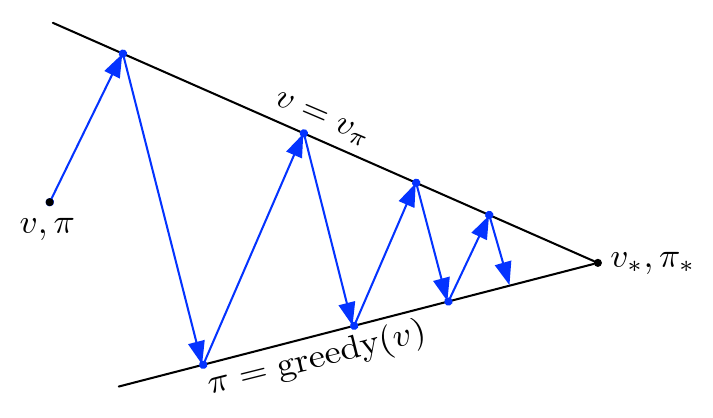
\includegraphics[scale=0.5]{GPI1.png}
    \caption{Illustration of the general policy iteration mechanism.\\Source: \citep{sutton2018}}
    \label{fig:GPI1}
    \todo[inline,color=cyan]{\textbf{To LAA:} Esta figura peguei diretamente do livro do \cite{sutton2018}, mas pretendo modificá-la ainda, evidenciando que o processo de avaliação (evalation) não precisa ser completo (a linha azul para cima não precisa ir até a preta).}
  \end{figure} 

The term \textit{generalized policy iteration} is used to designate the general ideia of letting policy evaluation an policy improvement process interact, independent of the number of steps and other details of the two process. This idea is represented in figure \ref{fig:GPI1}, where the evaluation and improvement in GPI are seen in terms of two goal, illustrated as the two black lines. The superior line represents the policy evaluation results and the inferior line, the policy improvement. Each blue line pointing to top right represents the iterations of policy evaluation before the policy improvement. The blue lines pointing to bottom right represents the policy improvement. As shown in the figure, driving toward one goal causes to move away from the other goal, e.g. making the policy greedy in respect to value function in general makes the value function incorrect for the new greedy policy and making value function evaluation typically causes the policy to be no longer greedy. But if the process continue, the processes is inevitably brought closer to the overall goal of optimality.


\section{Reinforcement Learning}
\label{sec:RL}

The basic ideas discussed about DP in previous sections can be extended to the case where no model of the system (or environment) to be controlled is unknown. This extension results in a methodology known as reinforcement learning (RL). The objective of reinforcement learning is estimate value functions and find optimal policies without the completely knowledge of the environment, as DP does. To reach this objective, RL uses actual experience, acting on the environment through an action, or the control action, and observing the imediate return, or cost.
% TODO: colocar figura aqui The figure \ref{fig:RLinteraction} exemplifies this interaction.

Two main approaches to learn the optimal policy from actual data can be defined as basis approaches to many RL algorithms.
They are the \textit{Monte Carlo (MC)} and  \textit{Temporal Difference (TD)} approaches.
Monte Carlo Methods requires only the sample sequence of states, actions and rewards from actual or simulated experience with the environment.
They uses the fact  that the value function (or cost-to-go) is the expected value of the return, expressed in \eqref{eq:cost_fun_return}. 
Using the sample sequence mentioned above, MC methods solves the RL problem based on the average sample returns in place of the true expected value, that is unknown.
The averaging sample return is updated after an episode completely occur.
% \todo[inline]{Colocar aqui o pq de nao aprofundar em MC metodos neste texto, e sim em TD.} Acho que já coloquei abaixo.
For a valid replacement of the expected value in \eqref{eq:cost_fun_return} with the sample return, the \textit{law of large numbers} needs to be applicable, i.e., a necessary condition to the sample return converges to the expected return is that the number of visits to each state $x_k$ goes to infinity. 
The problem of visit every state (or every state-action pair for control problems) is known as the \textit{exploration} problem and is inherent in RL problems and will be discussed with some more details in section \ref{sec:expandexp}.
The prediction problem (the computation of $J_\pi(\vx_k)$ and $Q_\pi(\vx_k,u_k)$), the policy improvement and the control problem (e.g.\ policy or value iterations) discussed in section~\ref{sec:DP} for DP can be adapted to be used in MC.

But, for dynamical systems control purposes, wait for an entire episode finish to update de value function and then improve policy can be a problem, mainly for real time problems.
The TD methods, solves this problem, i.e.\ updates the value function earlier, without the need of wait the entire episode to finish.
For these reason, in this thesis some TD methods will covered in detriment of the MC ones.

The next sessions presents the basis of TD methods and some extensions. 

% \subsection{Policy Iteration and Value Iteration in RL}
% \label{sec:PoVaIRL}

\subsection{The Exploration and Exploitation Dilemma}
\label{sec:expandexp}

If the policy $\pi(\vx)$ is deterministic, i.e. the actions probability matrix are composed of only 0's and 1's, following $ \pi$ will result only in the observation of the returns from one action at each state and the guarantee that every action-state pair can be visited infinite times, required for convergence of policy evaluation when using action values will not be satisfied.
% \todo{and the action and states transitions probability distributions are unknown?}
The problem of visit every action-state pair infinity times when times goes to infinity is known as the problem of \textit{maintainig exploration}. So, for problems involving action-values functions prediction, is desirable that every action is taken with a probability grater than zero, i.e., $1 > \pi(x_k) > 0$ for all $\vx_k \in \Omega_k$ to guarantee convergence in prediction. But in the opposite way, for policy improvement, is desirable that the policy be greedy, i.e. the best action in the sense that minimizes the action-value function, $Q(\vx,u)$, which results in a deterministic policy\footnote{one exception is for that cases which two or more equally valued minimum action-value function}. This is known as the \textit{exploitation problem}. This results in the \textit{exploration and exploitation dillema}.

Aiming to guarantee convergence of policy evaluation and improvement, some actions should be taken to guarantee exploration and exploitation at some degree. For RL problem, as will be treated in future sections, this dilemma can be solved with some different strategies.
One possible solution, is starting every episode, for episodic cases, in a random state, with probability grater then 1 for every state. But this solution is not feasible for continuing cases, or most dynamical control cases where the start state can not be chosen arbitrary. A most useful solution is to consider the policy as an \textit{$\epsilon$-soft} policy, where random actions are taken with $\epsilon$ probability, and deterministic actions, following the evaluated policy, are taken with probabilities  $1-\epsilon$. A common choice of  $\epsilon$-soft policy on control problems, where the policy must be improved, is use a particular  $\epsilon$-soft policy called  $\epsilon$ \textit{-greed}, where actions are chosen between a randomly one, with $\epsilon$ probability, and a \textit{greedy} policy, aiming to minimize the value function, based on evaluated policy.  
The last approach is common on what is called \textit{on-policy} control, where the policy followed by the agent are the same as the improved policy. 

Another possible solution to the exploration, exploitation dilemma is to use the \textit{off-policy} approach, where the system follows a exploratory policy, but a different policy is improved. This approach is useful for practical problems, where the system learns a better policy whiling follows a more conservative, but exploratory one. However as will see, this approach can results in convergence problems when used with value function approximation, as will see in section \eqref{sec:funcApprox}.

\subsection{Temporal-Difference Learning}
\label{sec:TDlearning}

Temporal-Difference Learning, as Monte Carlo methods, learns direct from sampled data without the need of a system model, but unlike MC methods, they don't wait for the entire episode to complete to update the estimate of the value functions $J_\pi(\vx_k)$  or  $Q_\pi(\vx_k,u_k)$, behaving, in this sense, more like DP methods. 

To reach the objective of find an optimal (or near to optimal) control policy, i.e. to solve the control problem, TD learning methods follow the pattern of the GPI where the policy is evaluated an improved, as presented in section 
% \todo{Colocar uma secao sobre GPI. Colocado: section \eqref{sec:GPI}}
\ref{sec:GPI}. 
To pursuit the optimal or quasi-optimal control, first the problem of prediction, or policy evaluation, in TD sense will be discussed. As in DP case, the policy improvement is presented in sequence, for finally, deal with some control approaches with use of TD learning.

The simplest TD method, known as \textit{one-step} TD, or \textit{TD(0)}, updates their state value function $J(x_k)$ as
\begin{equation}
  J(\vx_k) \gets J(\vx_k) + \alpha\left[r_k(\vx_k) + \gamma J(\vx_{k+1}) - J(\vx_k)\right]
\label{eq:TDupdate},
\end{equation}
% \todo{Estou com impressão que não falei sobre $\alpha$. Olhar isso. Colocado como nota de rodape.}
as long as the transition to state $x_{k+1}$ is completed and the imediate cost $r_k$ is spent.
The $\alpha$ term is a step-size parameter that, for convergence, in general needs to satisfy the standard stochastic approximation conditions\footnote
{ 
  A well-known result in stochastic approximation theory gives the conditions required to assure convergence of a sequence $\{\alpha_n(a)\}$ with probability 1:
  \begin{equation}
      \sum_{i=1}^\infty \alpha_i(a) = \infty \quad \text{and } \quad \sum_{i}^\infty \alpha_i^2(a) < \infty
    \label{eq:stochAppTeor},
  \end{equation}
  where first condition is required to guarantee that the steps are large enough to eventually
  overcome any initial conditions or random fluctuations and the second one guarantees
  that eventually the steps become small enough to assure convergence.
}.

The term $ r_k(x_k) +\gamma J(x_{k+1})$ in right hand side of \eqref{eq:TDupdate} is called the \textit{target} 
% \todo{Colocar aqui o pq to target? Comparando com outros casos? Ex. Caso MC.}
of TD method and the quantity inside the brackets measures the difference between the estimated value of $x_k$, 
% \todo{Usar um ``tilde'' em $J$ para enfatizar que é uma aproximacao?}
$J(x_k)$, and the better estimate given by the target. This difference is called the \textit{TD error} and can be defined as
\begin{equation}
  \delta_k \doteq r_k(x_k) +\gamma J(x_{k+1}) - J(x_k)
  \label{eq:TDerror}.
\end{equation}

TD error measures the estimation error \textit{made at that time} and, as it depends on the time $k+1$, it is not available until this time step is reached. A procedure for TD(0) is presented in Algorithm \ref{alg:TD0}

\begin{algorithm} % TD(0)
  \caption{Pseudo code for Policy evaluation using TD(0)}\label{alg:TD0}

  $\pi \gets $ policy to be evaluated \\
  $\alpha \gets $ value $\in \mathopen[0,1 \mathclose]$ \\
  $J(\vx) \gets$ arbitrary value $\forall \vx \in \Omega$ except for $J(terminal) = 0$

  \For{each episode}
  {
    Initialize $\vx_k$ \\
    \While{$\vx_k$ is nonterminal}
    {
      $u_k \gets$ action given by $\pi(\vx_k)$ \\
      Take control action $u_k$, observe $r_k$ and $\vx_{k+1}$ \\
      $J(\vx_k) \gets J(\vx_k) + \alpha\left[r_k(\vx_k) + \gamma J(\vx_{k+1}) - J(\vx_k)\right]$ \\
      $k = k+1$
    }
  }
  % \Return $J(x_k)$ for all $x_k \in \Omega$ \tcp*{Optimal Policy}
\end{algorithm}

\todo[inline]{Colocar mais sobre convergencia do TD(0)?} 

\subsection{On-Policy TD Control: Sarsa} 
\label{sec:sarsa}

% \subsubsection{Sarsa}
% \label{sec:sarsa}

For control purposes is desirable to learn an action-value function, or the Q-function, rather than the state-value function. The same procedure used to learn the state-value function on section \eqref{sec:TDlearning} can be used to learn the Q-function. But the state-action pair to state action pair transitions is used, instead of the state to state transitions used in TD earlier. Both the cases can be represented as Markov chains with rewards, and the same theorems assuming convergence of state values under TD(0) can be applied for action-values updates, given by
\begin{equation}
  \tqxu \gets \tqxu + \alpha\left[r_k(x_k,u_k) + \gamma \tqxuo - \tqxu\right]
\label{eq:Sarsa}.
\end{equation}
\todo[inline]{A partir daqui comecei a usar til para representar valores aproximados. Fazer isso para trás também! Para J.} 
The update of \eqref{eq:Sarsa} is done after every transition from a nonterminal state $x_k$, and $\tqxuo = 0$ if $x_k$ is terminal. This algorithm is known as 
Sarsa\footnote{The name Sarsa comes from the fact that the transitions are given as an alternate sequence of state-action-reward for stage $k$ and state-action for stage $k+1$, i.e,  $\{x_k,u_k,r_k,x_{k+1},u_{k+1}\}$, and a common notation used for states, actions and rewards on RL community is $S$,  $A$,  $R$, respectively, resulting in the sequence $\{ S_k, A_k, R_k, S_{k+1}, A_{k+1} \}$, i.e. S-A-R-S-A.} 
in RL community. The Sarsa algorithm basis is presented in the Algorithm \ref{alg:sarsa}.

\begin{algorithm} % === SARSA === Algorithm
  \caption{Pseudo code for Sarsa to estimate $\approx Q^*$ } \label{alg:sarsa}
  \DontPrintSemicolon

  $\alpha \gets  $ value $ \in  (0,1)$ \\
  $\tq(x,u) \gets$ arbitrary value $\forall \vx \in \Omega$, $u \in \mathcal{U}$, except for $\tq(terminal,\cdot) = 0$

  \For{each episode}
  {
    Initialize $\vx_k$ \\
    % Choose $u_k$ from $\vx_k$ using policy derived from $\tq$ (e.g.,  $\epsilon$-greedy)
    $u_k \gets$ action from $\vx_k$ using policy derived from $\tq$ (e.g.,  $\epsilon$-greedy) \\
    \For{step $k=0,\ 1,\ \dots, $ until the end of episode}
    {
      Take control action $u_k$, observe $r_k,\ \vx_{k+1}$ \\
      $u_{k+1} \gets$ action from $\vx_{k+1}$ using policy derived from $\tq$ (e.g.,  $\epsilon$-greedy) \\
      $\tq(\vx_k,u_k) \gets \tq(\vx_k,u_k) + \alpha\left[r_k(\vx_k,u_k) + \gamma \tq(\vx_{k+1},u_{k+1}) - \tq(\vx_k,u_k)\right]$ \\
      % $k = k+1$
    }
  }
  % \Return $J(x_k)$ for all $x_k \in \Omega$ \tcp*{Optimal Policy}
\end{algorithm}

Sarsa converges to an optimal policy as long as all state-action pairs are visited an infinite number of times. This can be accomplished using an $\epsilon-$\textit{greedy} policy, what makes the policy converge to the optimal policy with probability 1.

\subsection{Off-Policy TD Control: Q-learning} 
\label{sec:qlearning}

One of the most used off-policy methods on RL is an off-policy TD control algorithm known as \textit{Q-learning} \citep{watkins1989}, where the value function update is defined by
\begin{equation}
  \tqxu \gets \tqxu + \alpha\left[r_k(x_k,u_k) + \gamma \min_{u\in \mathcal{U}_k} \tq(x_{k+1},u) - \tqxu \right]
  \label{eq:QlearningControl},
\end{equation}
resulting in an algorithm that learns the action-value function $Q$ that directly approximates $Q^*$, i.e. the optimum action-value function independent of the policy being followed. The requirements for convergence are that all action-value state pairs are visited and updated for the policy to be improved, as required for the policy improvement theorem (Theorem \ref{teo:polImprov}) and the stochastic approximation conditions on the sequence of step-size parameters. With this conditions satisfied, $Q$ has been shown to converge with probability 1 to  $Q^*$ for the tabular case \eqref{eq:QlearningControl}. The Algorithm \ref{alg:Qlearning} shows a procedure to Q-learning.

\begin{algorithm} % [Q-learning]
  \caption{Pseudo code for Sarsa to estimate $\tq \approx Q^*$ }\label{alg:Qlearning}
  \DontPrintSemicolon

  $\alpha \gets $ value $\in (0,1]$ \\
  $\tq(x,u) \gets$ arbitrary value $\forall \vx \in \Omega,\ u \in \mathcal{U}$, except for $\tq(terminal,\ \cdot\ ) = 0$

  \For{each episode}
  {
    Initialize $\vx_k$ \\
    % Choose $u_k$ from $\vx_k$ using policy derived from $\tq$ (e.g.,  $\epsilon$-greedy)
    \For{step $k=0,\ 1,\ \dots, $ until the end of episode}
    {
      $u_{k} \gets$ action from $\vx_k$ using policy derived from $\tq$ (e.g.,  $\epsilon$-greedy) \\
      Take control action $u_k$, observe $r_k,\ \vx_{k+1}$ \\
      $\tq(\vx_k,u_k) \gets \tq(\vx_k,u_k) + \alpha\left[r_k(\vx_k,u_k) + \gamma \min_{u \in \mathcal{U}_k} \tq(\vx_{k+1},u_{k+1}) - \tq(\vx_k,u_k)\right]$ \\
      % $k = k+1$
    }
  }
  % \Return $J(x_k)$ for all $x_k \in \Omega$ \tcp*{Optimal Policy}
\end{algorithm}

% TODO: Colocar as seguintes seções?
% \subsubsection{Q-learning}
%   \label{sec:qlearning}
% \section{$n$-step Bootstrapping?}%
%   \label{sec:n_step_bootstrapping}


\section{Function Approximation}
  \label{sec:funcApprox}

Until now, the value functions $J(\vx)$ and  $Q(\vx)$ was considered as a lookup table, i.e. the states was considered as \todo{não estou certo se a palavra seria \textit{discretizada} mesmo. Quantizada, talvez?} discrete and finite values in state space. In the same form, actions are considered as discrete values too. The tabular approach is useful for discrete in state-action systems, where the number of state-action pairs are relatively small. For systems with huge state-action pairs or where states are treated as continuous values, resulting in continuous a new approach is needed. To aim this objective, the concept of function approximation is introduced in this and next sections. First, in this section this approximation is done by what will be called value-function approximation. In this methodology, the value-functions (state-value and action-value) are approximated with continuous functions as described in sequence.
This type of approximation, make possible to represents continuous states and their related value functions, but they do not deal with continuous action spaces. To deal with continuous action spaces, policy gradient method are presented at the end of the section.

% a parameterized functional form, with parameters represented as a vector $\vpfa \in \R^d$, where $d$ is the number of parameters. This parametric approximation will be represented by $\Jfa_\pi(\vx,\vpfa)\approx J_\pi(\vx)$ for a policy $\pi$.

\subsection{Value-Function Approximation}
  \label{sec:valFunApp}

The methods discussed so far, all updates an estimated value function of a state toward an better prediction that includes the most recent data collected.
From now on, that better prediction will be called \textit{update target}.
The notation $x \mapsto T$, where $x$ is the state where the value function was updated an $T$ is the \textit{update target}, will be used.
This update indicates that the estimated value of $x$ should be more like the updated target  $T$.
For example, with this notation, the TD(0) update can be written as $x_k \mapsto r_k + \gamma \Jfa(\vx_{k+1},\vpfa_k)$\footnote
{
  here the parametric approximation $\Jfa(\vx,\vpfa_k)$ is used in place of the value function estimative $\hat{J} (\vx_k)$ of tabular method presented in Section~\ref{sec:TDlearning}.
}.
The update target represents the old value estimation updated with the most recent information (e.g., the imediate cost $r_k$ on TD(0) presented above).
\todo{Acho que faltou ``apresentar'' o vetor de parametros $\vpfa = \begin{bmatrix} \pfa_1 & \pfa_2 & \cdots & \pfa_d \end{bmatrix}^T $} 
A wide range of function approximation methods have been studied in scientific community, on last decades. This methods aim to reproduce the same input-output relation of a collected data.
Many of this existing methods of function approximations, some better then others, can be used for value  predictions on RL, using the $x \mapsto T$ of each update as a training example.
This value function predictions is used as an estimated value function.
For RL purposes, methods that can learn online and that are able to handle with nonstationary target functions are, in general, required.
Most of the function approximation methods are parametric, in the sense that they seeks for a parametric function that approximates of the true value function by adjusting the parameters until some objective is archived.
As in this thesis we deal only with parametric methods, only this class of functions approximations will be studied.
Besides the parametric or nonparametric classes, function approximation methods can be classified as \textit{linear methods} and the \textit{nonlinear methods}.
In booth of this classes, the objective is to find a parametric function that approximates the value functions for, in general, huge state spaces, continuous or not, that makes difficult or impossible to be treated as a lookup table.
Basically, the difference between this two linear and nonlinear methods are that, in the former, the functions are linear in the parameters, and in the last, not.
In the next sections some of this methods are briefly presented, starting with the linear ones that, as will discussed later, in general, presents more convergence guarantees.

When using function approximation there is far more states than parameters, so an update at one state affects many others and is not possible to get the values all exactly correct.
To deal with it, is common to specify a state distribution $\mu(\vx) \ge 0,\ \sum_\vx = 1$, representing how much the error in each state are valuable.
So the difference between the approximate values $\Jfaxp$ and the true value  $J_\pi(\vx)$ is defined as the \textit{Mean Squared Value Error}, denoted here with $\overline{VE}$, and expressed as
\begin{equation}
  \overline{VE}(\pfa) \doteq \sum_{\vx \in \Omega} \mu(\vx) {\left[ J_\pi(\vx) - \Jfaxp \right]}^2
  \label{eq:VE}.
\end{equation}
The distribution $\mu(\vx)$ is called  \textit{on-policy distribution} and is commonly taken to be the fraction of time to be spent in $\vx$.

As mentioned earlier, there is a wide range of function approximation methods that can be used in reinforcement learning.
Here the methods based on gradient principles, like linear gradient descent methods will be explored, once they are used in this work.
In next sections, a brief about stochastic-gradient and semi-gradient methods is presented.
In sequence, some basics off function approximation for linear and non linear methods are presented as well. 

\subsection{Stochastic-gradient Methods}%
  \label{sub:stochastic_gradient_methods}

Stochastic-gradient descent (SGD, for short) methods are the most used of all approximation methods well suited for reinforcement learning.
In this methods, the approximate value function $\Jfaxp$ is a differentiable function of the parameter vector  $\vpfa$ for all  $\vx \in \Omega$. 

Assuming that the states are sampled (one at a time or in a batch way), the goal is to minimize the $\overline{VE}$, given in \eqref{eq:VE}, trying to minimize the error over the observed samples.
To do that, SGD methods adjust the parameter vector $\vpfa$ after each sample by a small amount in the direction which the error are most reduced, what can be expressed as
 \begin{align}
   \vpfa_{k+1} &\doteq \vpfa_k -\frac{1}{2}\alpha\nabla\left[J_\pi(x_k)-\Jfaxpk\right]^2 \label{eq:SGD_1}\\
            &= \omega_k + \alpha \left[J_\pi(x_k) - \Jfaxpk\right]\nabla\Jfaxpk
   \label{eq:SGD_2},
\end{align}
where $\alpha > 0$ is a step size parameter and $\nabla f(\vpfa)$, represents the gradient of any scalar function $f(\vpfa)$, expressed as a column vector given by
 \begin{equation}
  \nabla f(\vpfa) \doteq \left(\frac{\partial f(\vpfa)}{\partial\pfa_1},\ \frac{\partial f(\vpfa)}{\partial\pfa_2},\ \dots,\ \frac{\partial f(\vpfa)}{\partial\pfa_d} \right)^T
  \label{eq:grad}.
\end{equation}
So, SGD is a gradient descent method because they take a step in $\vpfa_k$ proportional to the negative gradient of the sampled squared error \eqref{eq:SGD_1}, and stochastic because the update is done in only a single sample, which might have been selected stochastically.
Over many samples, the overall effect is to minimize an average performance measure, like $\overline{VE}$ \eqref{eq:VE}.

The convergence to, at least, a local minimum of the performance measure, is guaranteed if $\alpha$ decreases over time in such a way that the  \textit{standard stochastic approximation conditions} (see footnote in section \eqref{sec:TDlearning}) are satisfied.

In \eqref{eq:SGD_1} and \eqref{eq:SGD_2}, the true state-value function $J_\pi(\vx)$ was used.
But this value is unknown on RL methods and the target $T_k$ is used in place of  $J_\pi(\vx)$, yielding in the following general SGD method 

\begin{equation}
\vpfa_k \doteq \omega_k + \alpha \left[T_k - \Jfaxpk\right]\nabla\Jfaxpk
\label{eq:genSGD}.
\end{equation}
Again, the convergence guarantees are satisfied under stochastic approximation conditions for a decreasing $\alpha$, but only if $Tkk$ is an  \textit{unbiased} estimate, i.e. $ \mathbb{E}[T_k|\vx_k=\vx] = J_\pi(\vx_k)$.
This is the case for Monte Carlo RL methods, but isn't the case for TD RL methods.

In TD RL methods, the target $T_k$ depends on the current value of the parameter vector  $\vpfa_k$, which results in a biased estimation and do not produces a true gradient-descent method.
The step from  \eqref{eq:SGD_1} to \eqref{eq:SGD_2} isn't valid in this case, because it relies on the independence of the target on $\vpfa_k$.

So, TD RL stochastic gradiente methods, or other methods that relies on 
% \todo{colocar significado de bootstraping aqui? Acho que não coloquei ainda. Checar.}
bootstrapping\footnote{bootstrapping methods are methods where bases they update in part on an existing estimate.}, that uses the update \eqref{eq:genSGD} are called \textit{stochastic semi-gradient methods}.

% TODO: Bootstrapping Update targets that include existing estimates (as in dynamic programming or TD methods) rather than relying exclusively on actual rewards and complete returns (as in MC methods).

Although semi-gradient methods do not converge as robust as the gradient methods, it converges reliably in linear case presented on next section.
Furthermore they results in faster learning and enables the learn to be continual and online without waiting for the end of the episode, which is good for continuing problems.
\todo[inline]{Colocar algoritmo para o TD(0) aqui? Acho que vou deixar para o caso do controle (SARSA, ou algo do tipo). Está ficando com muito algoritmo.}  


\subsection{Linear Function Approximation Methods}%
\label{sub:linear_function_approximation_methods}

Linear function approximation methods aim to approximate the state value function $J(\vx)$, for the prediction problem, or the action value function  $Q(\vx,u)$, for control problem, as parametric functions $\Jfa(\vx,\vpfa)$, or  $\Qfa(\vx,u,\vpfa)$, respectively. This approximation is done by means of the correct choice of the vector parameter $\vpfa$ that satisfies some criteria. The advantage is that, with a relative small size parameter vector $\vpfa \in \R^d$ and a same size real-valued vector $\vv(\vx) = \begin{bmatrix} x_1 & x_2 & \dots & x_d \end{bmatrix}^T $, the approximate value function can approximate the actual value function, for any real value of the state $\vx$. The vector $\vv(\vx)$ is called a \textit{feature vector} representing state $\vx$, with  $\vv_i(\vx) : \Omega \mapsto \R$ for each component $\vv_i(\vx)$. The state-value function are related with this vectors by the approximation
\begin{equation}
  \Jfaxp \doteq \vpfa^T \vv(\vx) \doteq \sum_{i=1}^d \pfa_i v_i(\vx)
  \label{eq:state-value-fa},
\end{equation}
where $\pfa_i$ and $v_i(\vx)$ are the parameter $i$ and the feature $i$, respectively, with  $i = 1,\ 2,\ \dots,\ d$.

For linear methods, the features form a linear basis for the set of approximate function, what make them basis functions. 
% \todo{Colocar aqui alguns dos possíveis métodos com referencias} Coloquei alguns parágrafos para a frente.
The diferente ways that features can be defined is what results in diferente methods of linear function approximations, as we see in next sections. But all of them share some basic properties, as will be presented in this section.

When using SGD updates with linear function approximation, the update \eqref{eq:genSGD} results in a particular simple for given as
\begin{equation}
  \vpfa_k \doteq \omega_k + \alpha \left[T_k - \Jfaxpk\right]\vv(\vx_k)
  \label{eq:lingenSGD},
\end{equation}
since the gradient $\nabla \Jfaxp = \vv(\vx)$ for a linear in parameter function.

One advantage of linear methods is that there is only one optimum (or a set of equals optimums for degenerated cases), and any method that guarantees the convergence to (or near to) a local optimum guarantees the convergence to (or near to) the global optimum.

The TD(0) using SGD linear function approximation, which is, in fact, a semi-gradient descent method, as discussed above, can be proved to converge the parameter vector to a point near of the global optimum \todo{Colocar esta prova? Talvez como anexo. A principio acho que não convém.}  \citep{sutton1988}, which is known as \todo{colocar o desenvolvimento do pq converge para um ``TD fixed point''?} \textit{TD fixed point}, and results, for the continuing case, in a $ \overline{VE}$ bounded as
\begin{equation}
  \overline{VE}(\vpfa_{TD}) \le \frac{1}{1-\gamma} \min_{\vpfa}\overline{VE}(\vpfa)
  \label{eq:meanSquaredValueError}. 
\end{equation}
This kind of convergence and bounds on $\overline{VE}$ applies to other on-policy bootstrapping methods as well. \citet{bertsekas1996} proved an analogous bound for the episodic case as well.
% Nevertheless, this convergences, is proved to linear function approximation using SGD updates for some on-policy bootstrapping (semi-gradient) methods with on-policy distribution. For off-policy cas

As stated before, the diferente ways that features can be defined results in diferente methods of linear function approximations, like \textit{Polynomials}, \textit{Fourier Basis} \citep{konidaris2011}, \textit{Coarse Coding} \citep{hinton1984,waltz1965}, \textit{Tile Coding} \citep{albus1971,watkins1989}, \textit{Radial Basis Functions} \citep{powell1987}, among others.

% Konidaris, Osentoski, and Thomas (2011) -> Fourier basis in a simple form suitable to reinforcement learning (with multidimentional continuous state spaces and functions that do not have to be periodic.
% Coarse coding -> Hinton (1984). Waltz and Fu (1965) example of this type of FA in RL
% Tile coding -> Albus(1971, 1981) -> introduced. Miller and Glanz (1996) -> deal with it.
% Radial Basis: Powell (1987), Broomhead and Lowe (1988), Poggio and Girosi (1989, 1990).

Here, in this work, only a brief introduction to polynomial and radial basis functions are given, since they are more relevant to this work. An introduction to another linear function approximations can be found on \citet{sutton2018}. In next sections this two methods are presented.

\subsubsection{Polynomials features for Function Approximations}
\label{sec:polynomial}

Polynomials are maybe, the most intuitive way to represents features for linear methods. This fratures representation are possible when problems can be expressed as numbers. Polynomials belongs to a family of features used for interpolation and regression, and might be the easiest way to introduce the concept of features construction.

Polynomials can be used to represent linear system, for example, a second order linear system, (such as model of a moving cart), could be represented with a two dimensional features vector $\vv(\vx) = \begin{bmatrix} v_1 & v_2 \end{bmatrix}^T $, with $ v_1 = x_1$ and $ v_2=x_2$, where $ x_1$ represents the first state variable and $ x_2$ (such as the cart position), the second (such as the cart velocity).

The example above shows the idea of a linear system representation with polynomials, but they could be used to represent nonlinear systems as well, since it continues to be linear in parameters. It enables for example, take into account interaction between the two states, or representation of affine functions in the original state numbers. For example, for a system with two states the feature $\vv_{\vx} = \begin{bmatrix} 1 & x_1 & x_2 & x_1x_2 \end{bmatrix}^T$ could be chosen, where $ x_1x_2$ represents the interaction and the term 1 allow the representation of the afine functions. More complexes features could be chosen as well, like one including terms like $ x_1^2$, $ x_2^2$, as well.

The general case can be state as follows.
Suppose a state vector $\vx \in \R^n$. For this $n$-dimensional state space, each polynomial basis of order  $k$ can be written as
 \begin{equation}
   v_i(\vx) = \prod_{j=1}^{n}x_j^{c_{i,j}} ,
\end{equation}
where each $c_{i,j}$ is an integer in the set $[0,k]$ for $n\ge 0$. This results in a order-$n$ polynomial basis for dimension $n$, and in  $(k+1)^{n}$ features.

In general, higher-order polynomials results in more accurate approximations, but features of order $k$ basis grows exponentially with the state space dimension $n$ (for $k>0$). In practice, generally, a subset the features are chosen based on some criteria, like prior beliefs about the nature of the system or some existent methods for polynomial regression.

\subsection{Nonlinear Function Approximations}
\todo[inline,color=cyan]{Saltei esta seção pois não sei se usarei (e por prioridades). Mas bem provável que sim. O foco aqui seria falar sobre aproximação por redes neurais, principalmente.} 
\subsection{On-Pollicy Control with function approximation}
\subsection{Off-Policy Control with function approximation}
\label{sec:offPoliceControlFA}




\subsection{Policy Gradient Methods}
\label{sec:PGM}


Policy gradient methods are function approximation methods as value-function approximation methods addressed on previous sections. However, instead of learn the values of actions an then select actions based on their estimated values, policy gradient methods learn a \textit{parametrized policy} directly. This allows to select actions without the use of a value function.

In policy gradient approach, the policy will be a parametrized function $\pi(u|\vx,\vt) =$ $\text{Pr}\left\{u_k=u | x_k = x, \vt_k = \vt\right\}$, i.e. the probability of taken the action $u$ at stage $k$. Where $\vt \in \R^{r}$ is the policy parameter vector, with $r = |\mathcal{U}|$.

The objective is to learn the policy parameter vector $\vt$ that minimizes some performance measure $P(\vt)$. It is done by updating the parameter vector in the direction whre the performance measure most decreases, i.e.
according to the gradient descent approach given by 
% To learn the policy parameter, these methods use the gradient of some performance measure $P(\vt)$, function of the parameter $\vt$ to update the parameter accoding to a gradient descent approach to minimize\footnote{sometimes is required to maximize the performance measure.l, resulting in a \textit{gradient ascent} $\vt_{k+1} = \vt_k + \alpha \apPG$.} the performance, the parameters are updated according to a gradient descent in $P(\vt)$:

\begin{equation}
\vt_{k+1} = \vt - \alpha \apPG
\label{eq:PGpar},
\end{equation}
where $\apPG \in \R^r$ is a stochastic estimate whose expectation approximates the gradient of the performance measure with respect to $\vt_k$.

Policy gradient methods can handle feasible discrete action spaces (where the action space is not too large an can be implemented in practice, as a lookup table), as huge  (where the number of actions are so large that tabular methods become impracticable) or continuous ones (with infinite number of actions).

If the action space is small enough a natural to define the policy as a numerical lookup table function $h(\vx,u\vt) \in \R$ for each state-action pair, commonly called as \textit{preferences}.
The idea is that the actions with highest preferences in each state presents higher probabilities to be selected. 
One example is an exponential distribution parametrization known \textit{soft-max in action preferences}, where
\begin{equation}
  \pi(u|\vx,\vt) = \frac{\exp{\left(h(\vx,u,\vt)\right)}}{\sum_{b \in \mathcal{U}} \exp{\left(h(\vx,b,\vt)\right)}}
\label{eq:softmax}.
\end{equation}
The actions preferences can be parametrized arbitrary, as a neural network, or linear in feature, or another method described in section \eqref{sec:funcApprox}.
If linear in features the preferences is written as
\begin{equation}
  h(\vx,u,\vt) = \vt^T\vv(\vx,u),
\end{equation}
using features vectors $\vv(\vx,u) \in \R^r$ constructed with one of the methods cited at end of section \eqref{sub:linear_function_approximation_methods}.

The main advantages of this kind of policy parametrization is that it enables to find stochastic optimal policies (whereas action-value methods can't do naturally), but can be used to approach a deterministic policy as well, where the actions are selected in an $\epsilon$-greedy manner.

\todo[inline,color=cyan]{ Falta coisas aqui ainda. Na verdade acho que essa abordagem usando Policy Gradient Methods deve acabar sendo mais útil para mim.}

% \begin{equation}
% \vt^T\vv(\vx,u), .
% \end{equation}

\subsubsection{Parametrization for continuous actions}

To deal with huge or continuous action spaces the general procedure is the same as the tabular case, but now, instead of learn the probabilities for each of the actions, the procedure look to learns the statistics of the probability distribution.

One common choice is to parametrize the policy as the normal probability density aver a real-valued scalar action, with standard deviation $\sigma(\vx,\vt)$ and mean $\mu(\vx,\vt)$ given by the following parametric function approximation:
\begin{equation}
  \pi(u|\vx,\vt) \doteq \frac{1}{\sigma(\vx,\vt)\sqrt{2\pi} } \exp{\left(-\frac{(u-\mu(\vx,\vt))^2}{2\sigma(\vx,\vt)^2}\right)} ,
\end{equation}
where the standard deviation and the mean is defined as a parametric function of $\vt$. For example, they can be defined as
 \begin{equation}
 \sigma(\vx,\vt) \doteq \exp{\left(\vt_\sigma^T\vv_\sigma(\vx)\right)} \quad \quad \text{and }
   \quad \mu(\vx,\vt) \doteq \vt_\mu^T\vv_\mu(\vx) ,
\end{equation}
with $\vt= \begin{bmatrix} \vt_\sigma & \vt_\mu \end{bmatrix}^T$,  $\vv_\sigma$ and $\vv_\mu$ representing a state feature vector that could be constructed using some method as cited on section \eqref{sec:funcApprox}.
Note that the standard deviation is a always positive value, for this reason is defined as an exponential function.


% \section{Infinite Horizon Problems}
% \label{sec:IHP}
%
% Since for dynamic control problems the trajectory of the system to be controlled is, in most of the cases, given in a infinite-step way, here we will try to deal with this case with more details. \todo[size=\tiny]{Talvez colocar isso na introdução do capítulo, falando que o objetivo do capítulo é chegar nesse ponto, mas para isso alguns conceitos fundamentais (casos mais simples?) devem ser tratado antes.}
%
% The main difference between the infinite horizon and the finite horizon RL problems, despite the obvious fact that in the former the number of stages are infinite, is that the system is stationary. It means that the state equation, the stage cost and the probability distribution of the random disturbance do not change from one to stage to the next \citep{bertsekasReinforcementLearningOptimal2019}.
%
% The stationarity assumption can be a problem to some practical time variant dynamical systems, but for many cases where the system parameters vary slowly with time, this assumption gives a good approximation.
%
% Infinity horizon problems, in general, results in simpler optimal policies than the finite case, which often presents a stationary behavior. But in the other hand the mathematical treatment can be more complex.
%
% The total cost of a policy $\vpi = {\mu_0, \mu_1, \dots}$ for a infinite horizon stochastic problem is given by
%
% \begin{equation}
  % J_\pi(\vx_0) = \lim_{N \to \infty} \E_{\vw_k} \left\{ \sum_{k=0}^{N-1} \gamma^{k} r(\vx_k,\vmu_k(\vx_k),\vw_k) \right\}
% \label{eq:JIH}.
% \end{equation}
% The term $\gamma$ is a positive scalar, and $\gamma <1$ results in a discount factor meaning that the present cost is more important than the future ones; and $\E_{\vw_k}$ means the expected value over all random disturbances  $\vw_k$, with $k = 0, 1, \dots$, until infinity. For now, the limit in \eqref{eq:JIH} is assumed to exists.
% In a procedure like that shown in sections \ref{sec:VaIDP} and \ref{sec:VaIRL}, the optimal cost-to-go function $J_N$ corresponding to $N$-stages finite horizon problem can be written according to the Value Iteration Algorithm that follows \todo{Tem coisas erradas aqui! 1- é $J_N$ mesmo? Não seria $J^*$? Acho que $J^*_N$ 2- a eq.  \eqref{eq:VIalgorithm} não é o caso ótimo!}
%
% \begin{equation}
  % J_{k+1}(x) = \min_{u\in \mathcal{U}} \E_{\vw_k} \left\{ r(\vx,\vu,\vw) + J_k\left(f(\vx,\vu,\vw)\right) \right\}, \qquad k = 0, 1, \dots, N-1
% \label{eq:VIalgorithm},
% \end{equation}
% starting from the initial condition $J_0(x)=0$, $\forall x$.
%
% The optimal infinite horizon can be expressed as
% \begin{equation}
  % J^*(x) = \lim_{N \to \infty}J_N^*(x)
% \label{eq:OptInfHOriz}.
% \end{equation}
%
% Minimization of \eqref{eq:JIH} can be accomplished with two strategies, denominated as
% \begin{itemize}
  % \item Stochastic shortest path problems (SSP)
  % \item Discounted problems.
% \end{itemize}
%
% % The next sections presents these to strategies.
% The next sections gives an introduction on these to strategies.
%
% \subsection{Stochastic Shortest Path}
%
% In Stochastic Shortest Path (SSP), is assumed that there is no discount factor, i.e. $\gamma = 1$ in~\eqref{eq:JIH} and there is a \emph{special terminal state t with cost free}, i.e.\ when the trajectory reaches that state, it remains there with no future cost. It can be formally written as
% \begin{equation}
  % p_{tt}(\vu) = 1, \quad r(t, \vu, t) = 0, \qquad \forall \ \vu \in \mathcal{U}
% \label{eq:SSP_1}.
% \end{equation}
% where \todo{colocar sobre essa probabilidade na seção~\ref{sec:SDP}?} $p_{ij}(\vu)$ means the probability of, at state $i$, taking a control action $\vu$, the system trajectory is driven to state $j$; and $r(i,\vu,j)$ represents the cost of the transition from state $i$ to  $j$ when control action $\vu$ is taken.
%
    % \begin{figure}[htpb]
        % \centering
        % % \includegraphics[width=0.8\textwidth]{}
        %     \begin{tikzpicture}[->,>=stealth',shorten >=1pt,auto,node distance=3cm, thick]
      \tikzstyle{every state}=[draw=black,fill=blue!20,text=black]
      % \tikzstyle{dots}=[thick,draw=none,fill=none,text=black]
      % \tikzstyle{place}=[draw=none,fill=none,text=black!75]
      % \tikzstyle{texto}=[draw=none,fill=none,text=black]
      \node[state] (i) {$i$};
      \node[state] (j) [right of=i] {$j$};
      \node[state] (t) [above of=i,xshift=1.5cm,yshift=-0.8cm] {$t$};

      \path[->]
          (i) edge [loop left] node {$p_{ii}(\vu)$} ( )
          (j) edge [loop right] node {$p_{jj}(\vu)$} ( )
          (t) edge [loop above] node {$p_{tt}(\vu) = 1$} ( )
          (i) edge [bend left] node {$p_{ij}(\vu)$} (j)
          (j) edge [bend left] node {$p_{ji}(\vu)$} (i)
          (i) edge node [left] {$p_{it}(\vu)$} (t)
          (j) edge node [right] {$p_{jt}(\vu)$} (t);
          % (C) edge node {c} (D);
    \end{tikzpicture}

        % \caption{Transition graph representing a MDP of a minimum SSP problem.}
        % \label{fig:stages}
      % \end{figure} \todo[inline]{Terminar. Melhorar caption. \st{Mexer na altura?} Contextualizar.}
%

  \clearpage
  \thispagestyle{empty}
  \cleardoublepage
% % }}} ------------------------------------------------------------------

% {{{ Capitulo 5 - Resultados Simulados
%!TEX root = Qualificacao.tex

%%%%%%%%%%%%%%%%%%%%%%%%%%%%%%%%%%%%%%%%%%%%%%%%%%%%%%%%%%%%%%%%%%%%%%%
%                              R a C S S                              %
%%%%%%%%%%%%%%%%%%%%%%%%%%%%%%%%%%%%%%%%%%%%%%%%%%%%%%%%%%%%%%%%%%%%%%%
% 2021-05-08

\chapter{Randomized Controller Structure Selection}\label{cap:CCS}
\vspace{-1cm}

% Frase citação inicial {{{1
% \begin{flushright}
% \begin{minipage}{0.7\linewidth}
%     \emph{``\dots''}
% \end{minipage}
% \end{flushright}
%
% \begin{flushright}
% Cicrano
% \end{flushright}
%
%\vspace{1cm}

% Intro CAP {{{2

In this chapter, an approach for the design of DDC controllers is presented, based on the RamSS methodology for the choice of structure and on the VRFT method for tuning the controller. This new approach is here called Randomized Controller Structure Selection, or RaCSS, for short.
% In this chapter, proposals for the design of DDC controllers, with regard to the choice of controller structure are presented. The methodology used, as well as the preliminary results obtained in a first stages of this research are presented.

In this research, focus has been given to the study and development of structure selection techniques for the model of feedback controllers in a DDC\@ design fashion.
The intention is, at first, in the scope of non-linear control systems, to adapt known techniques of structure selection in the area of systems identification to deal with the control case, where the system to be identified becomes the controller. To achieve these objectives, it was decided, to use polynomial models to represent the controllers, initially with NARX structures. This choice is convenient due to the structural flexibility characteristic and the ability of these models to describe non-linear systems~\citep{pearson1999, martins2013}.
% \begin{figure}[htpb]
% \centering
% \missingfigure{Pretendo colocar por aqui um diagramas (deve ser blocos) para ajudar.}
% % \includegraphics[width=0.8\textwidth]{}
% \caption{}
% \label{fig:Diagrama representativo}
% \end{figure}
%

As mentioned in Chapter~\ref{cap:cap2}, one of the main steps in the system identification procedure from data is the step of choosing the model structure. Works that aim to help on this task have been proposed, as is the case of the papers published  by~\cite{baldacchino2012,baldacchino2013} and \cite{falsone2014,falsone2015},
\todo{Vou colocar aqui mais referências neste sentido, de seleção de estruturas} 
in which a random approach is used in order to select the best candidates among the possible regressors in the formation of the model to be identified.

% As mentioned in Chapter~\ref{cap:cap2}, one of the main steps in the procedure of model system identification from data is the model selection step.  Studies that aim to deal with this task have been proposed, as is the case of studies developed by~\cite{falsone2014, falsone2015} in which a random approach, named RaMSS, is used in order to select the best candidates to compose a final model structure, among a class of possible regressors.
%
% \todo{Confirmar se o RaMSS original só é aplicável a NARX mesmo na sua forma original. Se for, falar aqui.}
More recently, ~\cite{retesNARMAXModelIdentification2019} extended the RaMSS strategy for choosing NARMAX model structures, which take into account the effect of noise on signals in order to reduce the polarization in parametric estimates.

In the scope of controller design based on data, more specifically by the VRFT method, in which the controller parameters are adjusted by conventional identification techniques such as OLS, ILS, IV, among others, the same problem of choosing the model structure occurs, with the difference that the model now represents the controller, and no longer the process. Therefore, analogies must be able to be made intended to use the RaMSS method in order to extend it for the purpose of identifying the most suitable structure for the controller.

In this sense, the present work has been directed to the study of the possibilities and consequences of using these technologies for control purposes, aiming to choose the most suitable controller structure.

The next section presents the basics of the methodology adopted for the RaCSS procedure, and then, some preliminary results obtained in the first stages of this research are studied.

\todo[inline]{Pretendo colocar um paragrafo aqui comentando o que será apresentado no restante do capítulo.} 


\section{Methodology}\label{sec:CSS_metod} \todo{Talvez colocar o Título como: ``The RaCSS Methodology''"?}
\todo[inline]{A terminar... Vou mexer no início e fim desta seção ainda, enquanto estiver traduzindo.} 

% Visando atingir o objetivo de se utilizar uma estratégia para estrutura e identificação paramétrica de controladores a partir de uma abordagem DDC, pretende-se neste trabalho, fazer uso das duas metodologias abordadas em capítulos anteriores: o VRFT, para sintonia de parâmetros do controlador e o RaMSS, para seleção da melhor estrutura do controlador.
In order to achieve the objective of using a strategy for structural and parametric identification of controllers from a DDC approach, this work intends to make use of the two methodologies covered in previous chapters: VRFT, for tuning controller parameters and RaMSS, to select the best controller structure.
% A partir de do estudo e adaptações de trabalhos anteriores \citep{retesNARMAXModelIdentification2019}, tem-se desenvolvido um algoritmo capaz de unir as duas estratégias com o objetivo de auxiliar tanto na seleção de estruturas, quando na sintodia de controladores não-lieares (ou lineares).
From the study and adaptations of previous works \citep{retesNARMAXModelIdentification2019}, an algorithm has been developed, capable of uniting the two strategies in order to assist in the selection of structures, as in the tuning of non-linear (or linear) controllers.
% O algoritmo tem servido de  framework para estudo e validação da abordagem proposta, a partir de simuações numéricas.
The algorithm has served as a framework for the study and validation of the proposed approach, based on numerical simulations.
% Neste sentido, parte dos esforços da pesquisa tem se voltado para a implemetação numérica deste framework.
In this sense, part of the research efforts has turned to the numerical implementation of this framework.
% Em uma primeira etapa, foi analisado o comportamento do algoritmo na identificação de modelos de processos, a partir do algoritmo RaMSS, como proposto originalmente.
In a first step, the behavior of the algorithm in the identification of process models was analyzed, using the RaMSS algorithm, as originally proposed.
% Alguns dos resultados de validação desta etapa são apresentados no Capítulo \ref{cap:cap2}, sob a forma do Exemplo \ref{ex:varHeater}.
Some of the validation results for this step was presented in Chapter \ref{cap:cap2}, in the form of Example \ref{ex:varHeater}.


% Uma vez validado o funcionamento do algorítmo, o método VRFT, discutido no Capítulo \ref{cap:VRFT} é acrescentado ao processo, de forma que o desempenho do RaMSS em selecionar estruturas para um controlador possa ser avaliado na prática.
Once the behavior of the algorithm has been validated, the VRFT method, discussed in Chapter \ref{cap:VRFT} is added to the process, so that the performance of RaMSS in selecting structures for a controller can be evaluated in practice.
% Nesta etapa, o algoritmo RamSS, utilizado no Capítulo \ref{cap:cap2} é ligeiramente modificado para lidar com a esimação paramétrica via VRFT, para primeiros testes de projeto de controladores.
In this step, the RaMSS algorithm, presented in Chapter \ref{cap:cap2} is slightly modified to deal with parametric estimation via VRFT, for the first tests of controller design.
% Neste cenário se espera alguns primeiros resultados, sem maiores compromissos com bons desempenhos, mas de são de grande valia para análise e comparação das modificações propostas. Alguns destes resuldados são apresentados pelos exemplos da seção \ref{sec:prel_results} a seguir, mais especificamente no exemplo \ref{ex:51}.
In this scenario, some first results are expected, without major commitments with good performances, but they are of great value for analysis and comparison of the proposed modifications. Some of these results are presented by the examples in the Section~\ref{sec:prel_results} below, more specifically in the Example~\ref{ex:sis2aord}.

% Como abordado no Capítulo \ref{cap:VRFT}, sob certas condições, o controlador pode ser identificado por procedimentos tradicionais de identificação de sistemas pelo método VRFT.
As discussed in Chapter \ref{cap:VRFT}, under certain conditions, the controller can be identified by traditional systems identification procedures using the VRFT method.
% Caso as condições necessárias não sejam satisfeitas (vide a Assumption \ref{ass:machedControl} -- matched control) um filtro pode ser projetado de forma que a minimização do índice de custo relativo aos sinais de entrada e saída do controlador, dado por $J_{VR}(\bm{\theta})$ resulte também na minimização do índice de custo $J_{MR}(\bm{\theta})$ relativo ao erro de rastreamento de um modelo de referência.
If the necessary conditions are not met (see Assumption \ref{ass:machedControl} - matched control) a filter can be designed so that the minimization of the cost index related to the input and output signals of the controller, given by $J_{VR}(\bm{\theta})$, also results in the minimization of the $J_{MR}(\bm{\theta})$ cost index related to the tracking error of a reference model.
% Esta relação é garantida pelo filtro desde que a estrutura do modelo não seja muito ``distante'' da estrutura ideal, i.e. desde que não seja muito subparametrizada.
This relationship is guaranteed by the filter as long as the model structure is not too ``distant'' from the ideal structure, i.e. as long as it is not too under-parameterized.

% Uma proposta da presente pesquisa é utilizar o procedimento RaMSS para tentar identificar a estrutura ideal para o controlador, ou pelo menos uma estrutura próxima que gere bons resultados ao se utilizar o procedimento VRFT. A identificação desta estrutura é feita a partir de dados colhidos sob a abordagem VRFT. Na tentativa de validar a proposta simulações são feitas em diferentes cenários.
A proposal of the present research is to use the RaMSS procedure to try to identify the ideal structure for the controller, or at least a close structure that generates good results when using the VRFT procedure. The identification of this structure is made from data collected under the VRFT approach. In an attempt to validate the proposal, simulations are carried out in different scenarios.
% Em um primeiro cenário o procedimento RaMSS é aplicado a um processo linear onde seu modelo e o modelo do controlador ideal são previamente conhecidos. O intuito aqui é analisar o comportamento do procedimento na seleção de regressores candidatos a um eventual controlador. Uma análise ao estilo Monte Carlo é aplicada ao processo em 2 casos: no primeiro, o procedimento é realizado sem influência de ruídos nos dados utilizados; no segundo, ruídos são acrescentados aos dados no intuito de simulação de um ambiente mais realista. O Exemplo \ref{ex:sis2aord} analisa estes casos.
In a first scenario, the RaMSS procedure is applied to a linear process where their model and the model of the ideal controller (matched control) are previously known.
The aim here is to analyze the behavior of the procedure in the selection of candidate regressors for a possible controller.
A randomized analysis is applied to the process in 2 cases: in the first, the procedure is performed without the influence of noise on the data used; in the second, noise is added to the data in order to simulate a more realistic environment.
Example \ ref {ex: sis2aord} analyzes these cases.

% O procedimento RaMSS foi originalmente proposto para lidar com identificação de processos, e não controladores.
The RaMSS procedure was originally proposed to deal with process identification, not controllers.
% A atualização do vetor de probabilidades para inclusão dos regressores (RIPs) é feita baseando-se em índices de desempenho visando avaliar a qualidade de predição do modelo.
The update of the vector of the Regressor Inclusion Probabilities (RIPs) is done based on performance indexes that evaluate the model's prediction quality.
% Esta predição é feita sobre dados de treinamento, utilizando uma versão exponencial do MSPE, e possivelmente, no intuito de aumentar a robustez, sobre dados de validação (free run simulation) por meio de uma versão exponencial do MSSE.
This prediction is made on training data, using an exponential version of MSPE, and possibly, in order to increase robustness on validation data (free run simulation), through an exponential version of MSSE.
% No entanto, para fins de controle, tais índices podem não ser os melhores.
However, for control purposes, these indexes may not be the best.
% Principalmente o índice baseado no MSSE, que exige maior custo computacional sob a proposta de promover melhoras na robustez do modelo identificado. O efeito é uma melhor predição do sinal de saída do do modelo identificado, mesmo quando excitado com sinais diferentes daqueles usados na identificação.
Mainly the index based on MSSE, which requires higher computational cost under the proposal to promote improvements in the robustness of the identified model. The effect is a better prediction of the output signal of the identified model, even when excited with signals different from those used in the identification.
% Apesar de carecer de mais estudos, a princípio este índice não parece trazer muitos benefícios quando utilizado para fins MSS do controlador, uma vez que o intuito final, no projeto de um controlador, é fazer com que o sinal de saída do processo (e não do controlador), tenha um comportamento desejado.
Despite the lack of further studies, at first, this index does not seems to bring many benefits when used for the controller's MSS (Model Structure Selection) purposes, since the main objective, in the design of a controller, is to make the process output (and not the controller's output), behave as desired.

% Neste sentido, propõe-se adaptações ao método RaMSS original visando objetivos mais adequados a MSS de controladores. Uma modificação estudada, é a substituição da versão exponencial do MSSE, dada por $J_s= e^{-K\cdot MSSE}$, por uma que leve em conta o rastreamento do sistema em malha fechada, um dos principais objetivos do controlador. Este novo índice é definido como
In this sense, it is proposed adaptations to the original RaMSS method aiming at objectives more suitable to MSS of controllers. A studied modification at the moment is the replacement of the exponential version of the MSSE, given by $J_s= e^{-K\cdot MSSE}$, by one that takes into account the closed-loop system tracking, one of the main objectives of the controller. This new index is defined as
\begin{equation}
  J_r=e^{-K\cdot MSTE},
  \label{eq:Jr}
\end{equation}
where $MSTE$, is defined here as the mean squared tracking error, given by
\begin{equation}
  MSTE = \frac{1}{N}\sum_{k=1}^{N} (y_{rm}(k)-y(k))^2.
  \label{eq:MSTE}
\end{equation} 

% O índice de desempenho final $\mathcal{J}$, utilizado em $\mathcal{I}$ (vide Equacão \ref{eq:desMedioReg}) para o cálculo dos RIPs, passa a ser calculado por:
The final performance index $\mathcal{J}$, used in $\mathcal{I}$ (see Equation \ref{eq:desMedioReg}) for the computation of RIPs, is now calculated by:
\begin{equation}
  \mathcal{J} = \alpha \mathcal{J}_r + (1-\alpha)\mathcal{J}_p
\label{eq:Jracss}
\end{equation}
% em que $J_p$ continua sendo o mesmo dado por \eqref{eq:Jp}, uma versão exponencial do MSPE. Este novo índice leva em conta o desempenho do controlador em malha fechada no processo de atualização dos RIPs.
where $J_p$ remains the same given by \eqref{eq:Jp}, an exponential version of MSPE. This new index takes into account the performance of the closed loop controller in the process of updating the RIPs.

% Uma vez que a escolha de estrutura é feita pelo método RaMSS modificado, incorporando elementos da estratégia VRFT, e que o intutito é a seleção de estrutura e parâmetros para controladores, batiza-se, aqui, esta estratégia de \textit{Randomized Controler Structure Selection}, ou RaCSS.
Since the choice of structure is made by the modified RaMSS method, incorporating elements of the VRFT strategy, and the aim is the selection of structure and parameters for controllers, this strategy is named here \textit{Randomized Controler Structure Selection }, or RaCSS.

% Resultados preliminares do uso deste índice são apresentados nesta qualificação. Os Exemplos \ref{ex:52} e \ref{ex:53} apresentam alguns destes resultados e uma análise geral é feita no Capítulo \ref{cap:Concl}. \todo{colocar a referencia correta aqui.}
Preliminary results from the use of this index are presented in next sections. Examples \ref{ex:52} and \ref{ex:53} show some of these results and a general analysis is done in Chapter \ref{cap:Concl}.

% Ressalta-se que os resultados apresentados são preliminares e conclusões concretas ainda não puderam ser apresentadas.
\todo{batizar o método de RaCSS.} 
% No Capítulo \ref{cap:Concl}, propostas para continuidade do trabalho, como inclusão de informações auxiliares ao procedimento, objetivando incorporar características previamente desejadas ou conhecidas para o controlador, assim como possivelmente o uso de estratégias de aprendizado por reforço, no intuito de reduzir o custo computacional devido ao uso de informações da malha fechada do controlador são apresentadas.
In Chapter \ref{cap:Concl}, proposals for continuing the work, such as the inclusion of auxiliary information to the procedure, aiming to incorporate previously desired or known characteristics for the controller, as well as possibly the use of reinforcement learning strategies, in order to reduce the computational cost due to the use of closed loop information from the controller are presented.

% Por fim, discussões a respeito de estabilidade, convergência, polarização e robustez são apresentadas, ainda não em um contexto de garantias, mas como conjecturas de passos que pretende-se aprofundar na sequência da presente pesquisa.
Finally, discussions about stability, convergence, polarization and robustness are presented, not yet in a context of guarantees, but as conjectures of steps that we intend to deepen in the sequence of this research.

\section{Preliminary Results}\label{sec:prel_results}

% -*- TeX-master: "/home/joao/DOUTORADO/GIT/Qualificacao/Qualificacao.tex" -*-
%!TEX root = ../Qualificacao.tex

%%%%%%%%%%%%%%%%%%%%%%%%%%%%%%%%%%%%%%%%%%%%%%%%%%%%%%%%%%%%%%%%%%%%%%%
%                 EXAMPLE 4.1 (51) - 2nd Order System                 %
%%%%%%%%%%%%%%%%%%%%%%%%%%%%%%%%%%%%%%%%%%%%%%%%%%%%%%%%%%%%%%%%%%%%%%%


% exemplo 51
\begin{exmp}[Second order Linear System -- continued.]\label{ex:sis2aord}

  Consider the 2nd-order linear system describe in Example \ref{exm:31}: 
  \begin{equation}
    \label{eq:sis2aord}
    y_k = a_1y_{k-1} + a_2y_{k-2} + b_1u_{k-1} + b_2u_{k-2}.
  \end{equation}
  % onde, para $i = 1,\ 2$, os termos $a_i$, $b_i$ $\in \R$, representam parâmetros constantes; $u_{k-i}$ e $y_{k-i}$ $\in \R$, os sinais de entrada e saída, respectivamente; e $k$ o índice temporal.
  According to the VRFT strategy (Chapter ~\ref{cap:VRFT}), one must first define a class of allowable controllers $\mathscr{C}$, containing the desired  structure, and define a reference model that expresses the desired close loop system's behavior.

  In this example, we want to analyze the use of the RAmSS algorithm directly, without modifications, in order to find the best structure for a controller designed from the VRFT strategy.
  In order to examine the behavior of the RaMSS Algorithm in finding the best set of regressors, we proceed as follows.

  A feasible reference model is defined, that is, with a relative degree equal to or greater than that of the process. For simplicity, a 1st order model with the same relative degree of the process is chosen, as Example \ref{exm:31}, given by the transfer function
  \begin{equation}
    M(z) = \frac{1-A}{z-A},
    \label{eq:mr_sis2aord}
  \end{equation}
  The parameter adopted here is the same as Exemple \ref{exm:31}, i.e. $A = -T_s/\tau_d = 0.8187$. 
  The ideal controller, represented by an ARX model, will be given by the structure composed of the regressors presented in \eqref{eq:exp31_uk}, represented here by
  \begin{equation}
    \label{eq:exp51_contIdeal}
    u_k = \theta_0e_{k} + \theta_1e_{k-1} + \theta_2e_{k-2} + \theta_3u_{k-1} + \theta_4u_{k-2},
  \end{equation}
  and will have the parameters shown in \eqref{eq:exp31_ideal_parameters}, described here as
  \begin{equation}
    \vtheta^\star= \begin{bmatrix} \theta^\star_0 & \theta^\star_1 & \theta^\star_2 & \theta^\star_3 & \theta^\star_4 \end{bmatrix}^T =  \begin{bmatrix} 0.181 & 0.308 &  0.145 &  0.19 & 0.81 \end{bmatrix}^T.
  \label{eq:ex51_ideal_parameters}
\end{equation}
Using the RaMSS algorithm, as discussed in the section ~\ref{sec:ramss}, the procedure is performed for 2 cases:
\begin{description}
  \item[case A] the universe set $\mathscr{M}$ is taken as all possible 3rd degree non linear models formed by the monomials up to 4 delays for input $\tilde{e}_k$ (virtual error) and output $\tilde{u}_k$ (virtual process input) collected data. No noise is considered in this case.
  \item[case B] the same case as case A, but now with a noise in the output, given by a gaussian distribution, i.e. $\nu \sim \mathcal{N}(\mu,\sigma)$, where $\mu=0$ is the mean, and $\sigma= 0.1$ is the standard deviation adopted. Note that the noise is added in the output, in a way that the model for the process is represented by an output error model (OEM).
\end{description}
The RaMSS procedure is applied to a data set of 700 samples, obtained via the VRFT procedure, in which the VRFT filter is considered to be unitary, i.e. the data is not filtered. The same data set is applied for the 2 cases. At each iteration, 100 candidate models are randomly chosen to be analyzed, using a Bernoulli process. The RIPs are updated in a maximum of 100 iterations, or until they all converge to a margin above 0.9 or below 0.1, i.e. the following stopping criterion is adopted:
\begin{align}
  \textbf{if } \left[iter<iter_{\max}\right] \textbf{ or } \left[\Delta_S < \frac{1}{2} \left(1-\min_{\forall \mu \in \bm{\mu}_k}{ \left| 2\mu -1 \right| }\right)\right] \textbf{ then} \text{, STOP the procedure.}
\label{eq:crit.par}
\end{align}
where $\Delta_S = 0.1$ is the convergence margin, $iter$ is the iteration number and $iter_{\max} = 100$ is the maximum allowed iterations.


Applying the procedure in both cases, the following controllers are obtained, for a specific realization:
\begin{align}
  % Para caso 24:
  \label{eq:ex51CasesAB}
  u_1(k) &= 0.636{u}_1(k-1) + 0.513{u}_1(k-2) + -0.321{u}_1(k-3) + 0.17{u}_1(k-4) \nonumber\\
      &\quad+ 0.181{e}_1(k) + 0.227{e}_1(k-1) + 0.045{e}_1(k-2) + 0.03{e}_1(k-4) \\
  u_2(k) &= 0.737{u}_2(k-1) + 0.242{u}_2(k-2) + -0.329{u}_2(k-3) + 0.32{u}_2(k-4) \nonumber\\
         &+ 0.175{e}_2(k) + 0.197{e}_2(k-1) + 0.049{e}_2(k-2) + 0.049{e}_2(k-3) + 0.059{e}_2(k-4)
  % u_1(k) &= 0.193{u}_1(k-1) + 0.805{u}_1(k-2)  \nonumber \\
         % &\quad + 0.001{u}_1(k-3) + 0.181{e}_1(k) + 0.307{e}_1(k-1) + 0.144{e}_1(k-2) \nonumber \\
  % u_2(k) &= 0.737{u}_2(k-1) + 0.242{u}_2(k-2) + -0.329{u}_2(k-3) + 0.32{u}_2(k-4)  \\
         % &\quad + 0.175{e}_2(k) + 0.  97{e}_2(k-1) + 0.049{e}_2(k-2) + 0.049{e}_2(k-3) + 0.059{e}_2(k-4)  \nonumber
  % u_1(k) &= 0.193{u}_1(k-1) + 0.805{u}_1(k-2) + 0.001{u}_1(k-3) \\
         % &+ 0.181{e}_1(k) + 0.307{e}_1(k-1) + 0.1441{e}(k-2), \\
  % u_2(k) &= 0.751{u}_2(k-1) + 0.241{u}_2(k-2) -0.33{u}_2(k-3) + 0.322{u}_2(k-4) \\
         % &+ 0.174{e}_2(k) + 0.197{e}_2(k-1) + 0.048{e}_2(k-2) + 0.049{e}_2(k-3) + 0.0591,
\end{align}
where the index subscribed to the variables represent the respective cases.

The table ~\ref{tab:exp51_param} sumarizes the simulation parameters used in \ref{alg:RaMSS}, for the 2 cases,
where $o$ is the maximum allowed degree for the regressors, $n_{\tilde{e}}$ is the maximum delay for the virtual error signal $\tilde{e}(k)$, $n_{\tilde{u}}$ is the maximum delay for the input signal of the sampled plant, $ N_p$ is the number of models chosen at each update of the RIPs, $ iter_{\max} $ is the maximum number of allowed iterations, $\Delta_S$ is the trashold for convergence of RIPs, $K$ is the gain for the performance indexes presented in \ref{eq:Js}, $\gamma_0$ is the initial gain of \ref{eq:gamma}, $\mu_{\min}$ and $\mu_{\max}$ are the minumum and maximum values allowed for the RIPs and $\nu$ is the noise added to the output.
\begin{table}[htpb]
  \centering
  \caption{Parameters for simulating the RaMSS algorithm of the example ~\ref{ex:sis2aord}}\label{tab:exp51_param}
  \begin{tabular}{c|c|c|c|c|c|c|c|c|c|c}
    Case & $o$ & $n_{\tilde{e}}$ & $n_{\tilde{u}}$ & $ N_p$ & $ iter_{\max} $ & $K$ & $\gamma_0$ &  $\mu_{\min}$ & $\mu_{\max}$ & $\nu$\\
    \hline
    A & $ 3 $ & $4$ & $4$ & $100$ & $100$ & $1$ & $2$ & $0.05$ & $1$ & $0$ \\
    B & $ 3 $ & $4$ & $4$ & $100$ & $100$ & $1$ & $2$ & $0.05$ & $1$ & $\mathcal{N}(\mu,\sigma)$
  \end{tabular}
\end{table}\\
\todo[inline]{MEXER NESTA TABELA AINDA! Valores estão errados. Já os modifiquei. Definir parâmetros, etc. Colocar os mais essenciais por aqui e os menos, no appendice. }

Note that the controllers presented in \eqref{eq:ex51CasesAB} are obtained for a specific realization of the procedure. All terms that end with the RIP above 0.95 are considered in the hundredth iteration.
Figure \ref{fig:ex51_RIPevol_2cases} shows the evolution of the RIPs for this realization.

\begin{figure}[H]
  \centering
  % 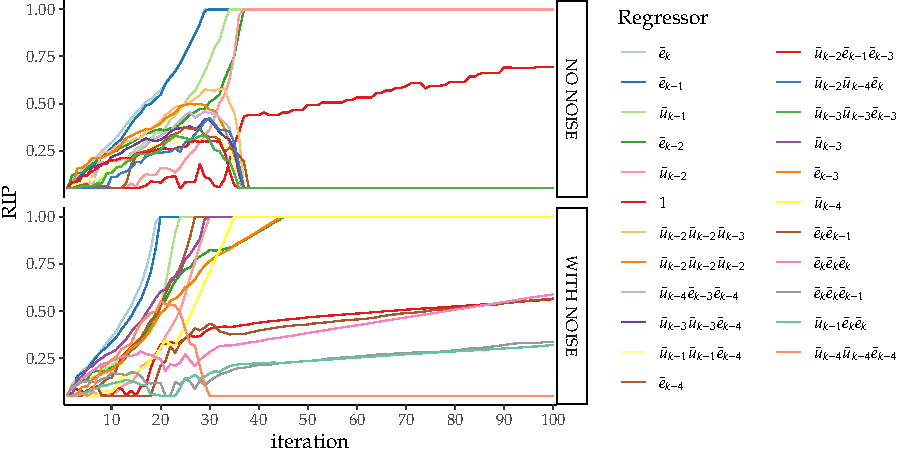
\includegraphics[width=\textwidth]{Figs/Cap5/ex51_rips_evol_2cases.tex.pdf}
  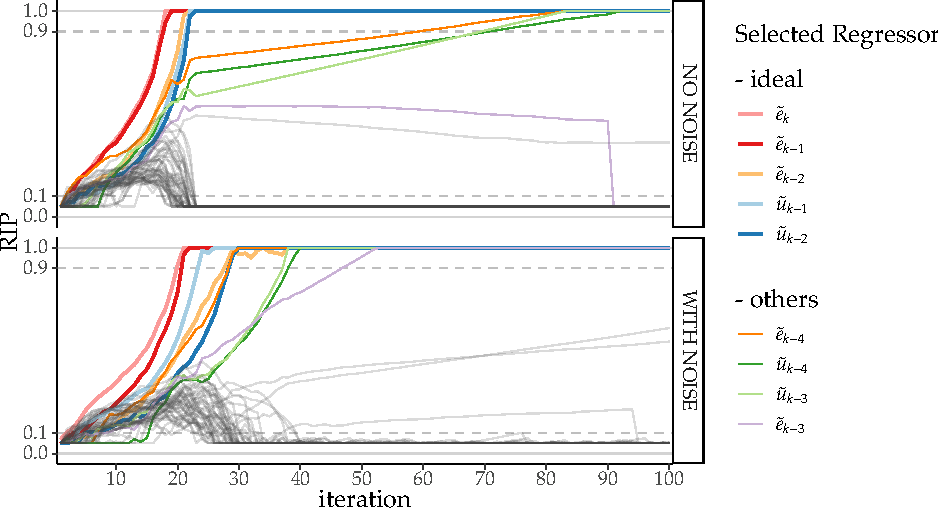
\includegraphics[width=\textwidth]{Figs/Cap5/ex51_rips.tex.pdf}
  \caption{Typical evolution of RIPs for choosing regressors for case 1 and 2.}
  \label{fig:ex51_RIPevol_2cases}
\end{figure}
\todo[inline]{Trocar esta figura} 

The ideal regressors are selected before the first 40 steps.
But as the iterations continue, the $\tilde{u}(k-3)$, $\tilde{u}(k-4)$ and $\tilde{e}(k-4)$ regressors continue to increase monotonically in value and eventually end up being selected.
The effect of including these terms, although in general they are small, deteriorates the desired behavior of the controller.
When considering noise in the measurement (case 2), the selection of non-ideal regressors occurs even earlier, as can be seen in the lower graph of \ref{fig:ex51_RIPevol_2cases}.
Part of this result is due to the worsening of parametric identification during the VRFT procedure, provoked by the polarization effect introduced by noise at the output. The result is that the regressor vectors are no longer orthogonal to the residuals and the OLS estimator becomes polarized. A strategy to mitigate this effect is to use non-polarized estimators, such as VI estimators, or even the ELS.

Figure ~\ref{fig:Figs-RespostaSist2aordNARX-png} shows the temporal response for the controllers identified in \eqref{eq:ex51CasesAB}, when the reference signal is taken as a square wave.

% The figure  shows the temporal response for a square wave in reference signal, for the 2 cases.
% Note que no Caso 1,

\begin{figure}[H]
  \sbox0{\blacksolidlinethin} \sbox1{\bluedashedline} \sbox2{\reddottedline} \sbox3{\blackdottedline} \sbox4{\bluedashdotedline} 
  \centering
  % 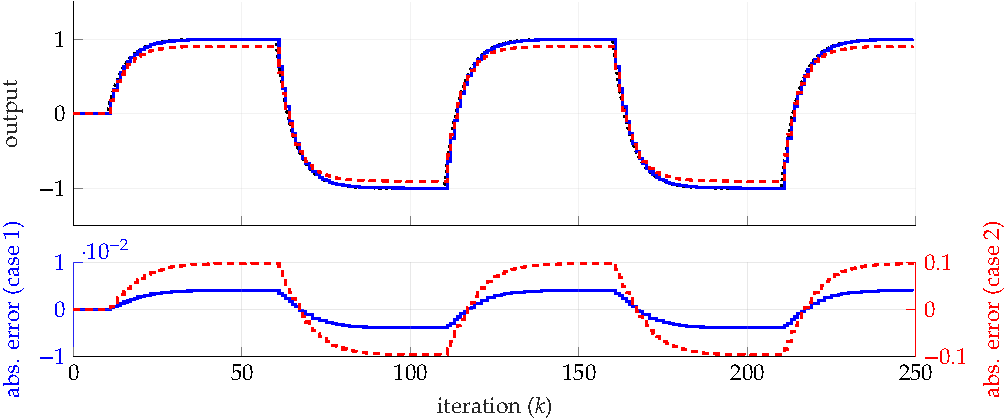
\includegraphics[width=1\textwidth]{./Figs/Cap5/ex51_resp_temporal_mf_editado.tex.pdf}
  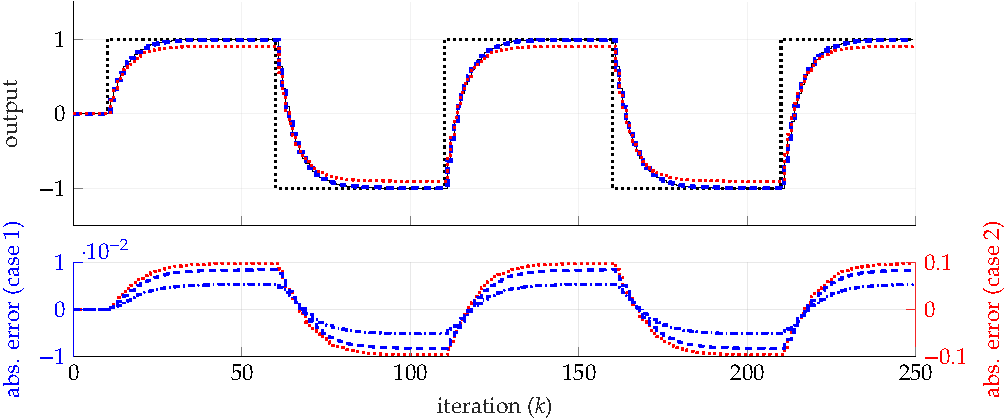
\includegraphics[width=1\textwidth]{./Figs/Cap5/ex51_resp_temporal_mf2.tex.pdf}
  % % This file was created by matlab2tikz.
%
%The latest updates can be retrieved from
%  http://www.mathworks.com/matlabcentral/fileexchange/22022-matlab2tikz-matlab2tikz
%where you can also make suggestions and rate matlab2tikz.
%
\begin{tikzpicture}

\begin{axis}[%
width=14.264cm,
height=3.794cm,
at={(0cm,2.206cm)},
scale only axis,
xmin=0,
xmax=250,
xtick={0,50,100,150,200,250},
xticklabels={{},{},{},{},{},{}},
ymin=-1.5,
ymax=1.5,
ylabel style={font=\color{white!15!black}},
ylabel={output},
axis background/.style={fill=white},
axis x line*=bottom,
axis y line*=left,
xmajorgrids,
ymajorgrids,
grid style={opacity=0.2}
]
\addplot [color=black, dotted, line width=1.0pt, forget plot]
  table[row sep=crcr]{%
0	0\\
10	0\\
11	0.181269246922028\\
12	0.329679953964359\\
13	0.45118836390597\\
14	0.550671035882772\\
15	0.632120558828547\\
16	0.69880578808781\\
17	0.753403036058387\\
18	0.798103482005331\\
19	0.834701111778401\\
20	0.8646647167634\\
21	0.88919684163767\\
22	0.909282046710587\\
23	0.925726421785669\\
24	0.939189937374778\\
25	0.950212931632137\\
26	0.959237796021625\\
27	0.966626730039678\\
28	0.972676277552694\\
30	0.981684361111263\\
32	0.987722660096921\\
34	0.991770252950971\\
37	0.995483419057393\\
41	0.997970569363702\\
47	0.999388747238868\\
60	0.999954600070225\\
61	0.637424335837267\\
62	0.340609659588267\\
63	0.0975983561783096\\
64	-0.10136247126897\\
65	-0.264257819357908\\
66	-0.397625250371675\\
67	-0.506817267601633\\
68	-0.596216130098412\\
69	-0.669409728114744\\
70	-0.729335577739135\\
71	-0.778398713730951\\
72	-0.818568212009893\\
73	-0.85145621558658\\
74	-0.878382635522144\\
75	-0.900428123593684\\
76	-0.918477442644473\\
77	-0.933254975223463\\
78	-0.945353795600482\\
79	-0.955259471919135\\
80	-0.963369553751249\\
81	-0.970009527157174\\
82	-0.975445877584235\\
84	-0.983540879531887\\
86	-0.988967121610102\\
88	-0.992604440449782\\
91	-0.995941230863423\\
95	-0.998176277468275\\
102	-0.999550275560608\\
110	-0.999909202201621\\
111	-0.637387167206128\\
112	-0.340579228486888\\
113	-0.0975734412997724\\
114	0.101382869846248\\
115	0.264274520300432\\
116	0.397638923946914\\
117	0.506828462578198\\
118	0.596225295770012\\
119	0.669417232331938\\
120	0.72934172167254\\
121	0.778403743958165\\
122	0.818572330411598\\
123	0.851459587448716\\
124	0.878385396169364\\
125	0.900430383820463\\
126	0.918479293161653\\
127	0.933256490298788\\
128	0.945355036039246\\
129	0.955260487504489\\
130	0.963370385242229\\
131	0.970010207924418\\
132	0.975446434949305\\
134	0.983541253144864\\
136	0.988967372050382\\
138	0.99260460832491\\
141	0.995941322995236\\
145	0.998176318865774\\
152	0.999550285769089\\
160	0.999909204262678\\
161	0.637387168893582\\
162	0.340579229868467\\
163	0.0975734424308996\\
164	-0.101382868920155\\
165	-0.264274519542226\\
166	-0.397638923326127\\
167	-0.506828462069933\\
168	-0.596225295353889\\
169	-0.669417231991247\\
170	-0.72934172139361\\
171	-0.778403743729797\\
172	-0.81857233022464\\
173	-0.851459587295636\\
174	-0.878385396044024\\
175	-0.900430383717861\\
176	-0.918479293077638\\
177	-0.933256490230008\\
178	-0.945355035982942\\
179	-0.955260487458389\\
180	-0.963370385204456\\
181	-0.970010207893495\\
182	-0.975446434923981\\
184	-0.983541253127925\\
186	-0.988967372039014\\
188	-0.992604608317293\\
191	-0.995941322991058\\
195	-0.998176318863898\\
202	-0.999550285768635\\
210	-0.999909204262593\\
211	-0.637387168893497\\
212	-0.34057922986841\\
213	-0.0975734424308712\\
214	0.101382868920183\\
215	0.264274519542255\\
216	0.397638923326156\\
217	0.506828462069961\\
218	0.596225295353918\\
219	0.669417231991275\\
220	0.72934172139361\\
221	0.778403743729797\\
222	0.81857233022464\\
223	0.851459587295636\\
224	0.878385396044052\\
225	0.900430383717861\\
226	0.918479293077638\\
227	0.933256490230008\\
228	0.945355035982942\\
229	0.955260487458389\\
230	0.963370385204485\\
231	0.970010207893495\\
232	0.975446434923981\\
234	0.983541253127925\\
236	0.988967372039014\\
238	0.992604608317293\\
241	0.995941322991058\\
245	0.998176318863898\\
249	0.999180567244224\\
};
\addplot[const plot, color=blue, line width=1.0pt, forget plot] table[row sep=crcr] {%
0	0\\
11	0.180977171837526\\
12	0.329172712212909\\
13	0.45031150992321\\
14	0.54950721174589\\
15	0.630603534262377\\
16	0.697071838198383\\
17	0.75129926836172\\
18	0.795887192211239\\
19	0.832113918402939\\
20	0.862042313411223\\
21	0.886239644815532\\
22	0.906320094899854\\
23	0.922499135273426\\
24	0.935950021055618\\
25	0.946791840399243\\
26	0.955778629339733\\
27	0.963064221517527\\
28	0.969052500940336\\
29	0.973959104837405\\
30	0.977943604763652\\
31	0.981248875948808\\
32	0.983902902127539\\
33	0.986123664527099\\
34	0.987898809353766\\
35	0.98938291118904\\
36	0.990577874726654\\
37	0.991563033579666\\
38	0.99237257824521\\
39	0.99302302327095\\
40	0.993573142885879\\
41	0.994002292764549\\
42	0.994375004464132\\
43	0.994660023006162\\
44	0.99491004110115\\
45	0.995101960911995\\
46	0.995267159859196\\
47	0.995398551232711\\
48	0.995506018603493\\
49	0.995597031866481\\
50	0.995666340606363\\
51	0.995729353060426\\
52	0.995774354984661\\
53	0.995817277218976\\
54	0.995847290647959\\
55	0.995875646946359\\
56	0.995896489317232\\
57	0.995914513739081\\
58	0.99592950784691\\
59	0.995940580406312\\
60	0.995951482435515\\
61	0.634003883369871\\
62	0.337620550089099\\
63	0.0953472448544233\\
64	-0.10303894571345\\
65	-0.2652285809788\\
66	-0.39816195207419\\
67	-0.506614475468581\\
68	-0.595788499822845\\
69	-0.668240060126379\\
70	-0.728095910664535\\
71	-0.776489090096334\\
72	-0.816649504165156\\
73	-0.849006521870962\\
74	-0.875907972279464\\
75	-0.897590947700024\\
76	-0.915564224598512\\
77	-0.930135072159629\\
78	-0.942111315794165\\
79	-0.951924405502382\\
80	-0.959893102619901\\
81	-0.966503635844077\\
82	-0.971811439975454\\
83	-0.976252980102885\\
84	-0.979803103504366\\
85	-0.982771300351828\\
86	-0.985161145199214\\
87	-0.987131422548657\\
88	-0.98875049439485\\
89	-0.990051322178317\\
90	-0.99115157956436\\
91	-0.992009815056377\\
92	-0.992755265095326\\
93	-0.993325252586487\\
94	-0.993825306183027\\
95	-0.994209118582432\\
96	-0.994539518302446\\
97	-0.994802294746677\\
98	-0.995017218301086\\
99	-0.995199252164724\\
100	-0.995337852432442\\
101	-0.995463889534307\\
102	-0.995553877257976\\
103	-0.995639731886712\\
104	-0.995699748235978\\
105	-0.995756465549192\\
106	-0.995798146571843\\
107	-0.995834194602935\\
108	-0.995864184425045\\
109	-0.995886325211501\\
110	-0.995908133508522\\
111	-0.633967273804899\\
112	-0.337591692291056\\
113	-0.0953226731259633\\
114	0.103058301629801\\
115	0.265244929159081\\
116	0.398175062764892\\
117	0.506625249266051\\
118	0.595797451149849\\
119	0.668247118158689\\
120	0.728102030832304\\
121	0.776493725318176\\
122	0.816653654829679\\
123	0.84900960826289\\
124	0.875910738485828\\
125	0.897593050066035\\
126	0.915566026255306\\
127	0.930136537077203\\
128	0.942112465237926\\
129	0.951925437303544\\
130	0.959893831175947\\
131	0.966504355793973\\
132	0.971811911211717\\
133	0.976253467082586\\
134	0.979803423931486\\
135	0.982771614147225\\
136	0.985161376691991\\
137	0.987131613667088\\
138	0.988750668125164\\
139	0.990051433495751\\
140	0.991151709211351\\
141	0.992009880262856\\
142	0.992755357103761\\
143	0.993325294868953\\
144	0.993825365970537\\
145	0.994209151088342\\
146	0.994539552657386\\
147	0.994802322807573\\
148	0.995017235142114\\
149	0.995199276392725\\
150	0.99533785939127\\
151	0.995463908745052\\
152	0.995553880291141\\
153	0.995639745123498\\
154	0.995699750932573\\
155	0.995756472981157\\
156	0.995798150277864\\
157	0.99583419749294\\
158	0.995864188932899\\
159	0.995886325370492\\
160	0.99590813792517\\
161	0.633967272955033\\
162	0.337591695755407\\
163	0.0953226724599574\\
164	-0.103058299551094\\
165	-0.265244929117785\\
166	-0.398175062008676\\
167	-0.506625248547522\\
168	-0.595797451309551\\
169	-0.668247117097962\\
170	-0.728102031391813\\
171	-0.776493724302242\\
172	-0.816653655361904\\
173	-0.849009607559282\\
174	-0.875910738755806\\
175	-0.89759304976053\\
176	-0.915566026223672\\
177	-0.930136537101305\\
178	-0.942112464997905\\
179	-0.951925437508748\\
180	-0.959893830868879\\
181	-0.966504356028963\\
182	-0.971811910957314\\
183	-0.976253467244817\\
184	-0.979803423791878\\
185	-0.982771614199692\\
186	-0.985161376669453\\
187	-0.987131613626559\\
188	-0.988750668181922\\
189	-0.99005143340699\\
190	-0.991151709296645\\
191	-0.992009880172304\\
192	-0.992755357175952\\
193	-0.993325294807619\\
194	-0.993825366007997\\
195	-0.994209151066315\\
196	-0.994539552658807\\
197	-0.994802322817804\\
198	-0.995017235119491\\
199	-0.995199276419669\\
200	-0.995337859360859\\
201	-0.99546390877299\\
202	-0.995553880266129\\
203	-0.995639745142142\\
204	-0.99569975091967\\
205	-0.995756472987182\\
206	-0.995798150277125\\
207	-0.995834197488733\\
208	-0.995864188940118\\
209	-0.995886325361141\\
210	-0.995908137934919\\
211	-0.633967272945597\\
212	-0.337591695763365\\
213	-0.0953226724537615\\
214	0.103058299547115\\
215	0.265244929119746\\
216	0.398175062008619\\
217	0.506625248546129\\
218	0.59579745131208\\
219	0.668247117094865\\
220	0.728102031395082\\
221	0.7764937242992\\
222	0.816653655364519\\
223	0.849009607557321\\
224	0.875910738757113\\
225	0.897593049759934\\
226	0.915566026223644\\
227	0.930136537101816\\
228	0.942112464997081\\
229	0.951925437509772\\
230	0.959893830867799\\
231	0.966504356029986\\
232	0.971811910956461\\
233	0.976253467245471\\
234	0.979803423791452\\
235	0.982771614199862\\
236	0.985161376669453\\
237	0.987131613626389\\
238	0.988750668182206\\
239	0.990051433406649\\
240	0.991151709297014\\
241	0.992009880171963\\
242	0.992755357176208\\
243	0.99332529480742\\
244	0.993825366008139\\
245	0.994209151066258\\
246	0.994539552658807\\
247	0.99480232281789\\
248	0.995017235119377\\
249	0.995199276419783\\
};
\addplot[const plot, color=red, dashed, line width=1.0pt, forget plot] table[row sep=crcr] {%
0	0\\
11	0.175057837660773\\
12	0.315108606907074\\
13	0.426588150709449\\
14	0.51956167119738\\
15	0.594286109260821\\
16	0.655135784739997\\
17	0.702527697924609\\
18	0.741838777618398\\
19	0.77225983010905\\
20	0.798373587886005\\
21	0.817964067832179\\
22	0.8350736083475\\
23	0.847611071714567\\
24	0.858723810104294\\
25	0.866922466539478\\
26	0.874060824457501\\
27	0.879513082557196\\
28	0.883999242995742\\
29	0.887673652014797\\
30	0.890462181039311\\
31	0.892949013964\\
32	0.894689964971832\\
33	0.896343978862291\\
34	0.897461842614717\\
35	0.898523537010391\\
36	0.899278919205585\\
37	0.899927562215879\\
38	0.900463534863803\\
39	0.90083967915939\\
40	0.901227428975886\\
41	0.90143979655096\\
42	0.901713732305325\\
43	0.901839323230234\\
44	0.902020253342215\\
45	0.902106347904407\\
46	0.902213540384309\\
47	0.902283235255084\\
48	0.902337553824992\\
49	0.902397723252136\\
50	0.902419819972835\\
51	0.902469326037533\\
52	0.902476441913677\\
53	0.902512513076459\\
54	0.90251623038057\\
55	0.902538032212703\\
56	0.902543914642166\\
57	0.902553458871893\\
58	0.902562340116049\\
59	0.90256361457989\\
60	0.902573698170528\\
61	0.552455445478785\\
62	0.272362786933741\\
63	0.0494007823988909\\
64	-0.136540247295017\\
65	-0.285990440390719\\
66	-0.407687067631656\\
67	-0.502470205440403\\
68	-0.581092278701334\\
69	-0.641932311178806\\
70	-0.694161189176867\\
71	-0.733339692463602\\
72	-0.767560412461251\\
73	-0.79263335075575\\
74	-0.814859956970821\\
75	-0.831256182941274\\
76	-0.845533232563184\\
77	-0.856437559375536\\
78	-0.865409538605803\\
79	-0.872758770170918\\
80	-0.878335140896809\\
81	-0.88330943754994\\
82	-0.886790649753493\\
83	-0.890099211291471\\
84	-0.892334474714488\\
85	-0.894458138169568\\
86	-0.895968736547701\\
87	-0.897266028287817\\
88	-0.898338051108368\\
89	-0.899090166389698\\
90	-0.899865869116638\\
91	-0.900290373633823\\
92	-0.900838455599256\\
93	-0.901089448591165\\
94	-0.901451449058101\\
95	-0.901623540769322\\
96	-0.901837971016619\\
97	-0.901977355190809\\
98	-0.902085960258347\\
99	-0.902206353892666\\
100	-0.9022504763999\\
101	-0.90234956258152\\
102	-0.902363722937849\\
103	-0.902435925631892\\
104	-0.902443313274432\\
105	-0.902486947330146\\
106	-0.902498697163736\\
107	-0.902517786090243\\
108	-0.902535559211117\\
109	-0.902538089185128\\
110	-0.90255827970293\\
111	-0.552437424800161\\
112	-0.272353669518367\\
113	-0.0493887280749448\\
114	0.136546275187442\\
115	0.285997795158806\\
116	0.407691694069229\\
117	0.502474143318068\\
118	0.581096134216409\\
119	0.641934087841918\\
120	0.694164336115279\\
121	0.733340374593951\\
122	0.767562741271121\\
123	0.792633684597831\\
124	0.814861425197137\\
125	0.831256561092516\\
126	0.845533945951161\\
127	0.8564380834612\\
128	0.865409719746452\\
129	0.872759366985946\\
130	0.87833504778024\\
131	0.8833099779593\\
132	0.886790497812001\\
133	0.890099595248756\\
134	0.892334392981667\\
135	0.894458332123122\\
136	0.895968764038798\\
137	0.89726606144643\\
138	0.898338162241629\\
139	0.899090103490011\\
140	0.899866010181398\\
141	0.900290283164196\\
142	0.900838576423098\\
143	0.901089379855762\\
144	0.901451521089001\\
145	0.901623515058702\\
146	0.901837990733185\\
147	0.901977369365483\\
148	0.902085942205645\\
149	0.902206390863569\\
150	0.902250442146482\\
151	0.902349602678896\\
152	0.902363691363718\\
153	0.902435954655999\\
154	0.902443295162755\\
155	0.902486959715276\\
156	0.902498694480471\\
157	0.902517783862891\\
158	0.902535567669759\\
159	0.902538078608103\\
160	0.902558292559149\\
161	0.552437412716728\\
162	0.272353680841377\\
163	0.0493887193443356\\
164	-0.136546268713317\\
165	-0.285997798625345\\
166	-0.407691692909395\\
167	-0.502474142154227\\
168	-0.581096136835015\\
169	-0.641934084084795\\
170	-0.694164340221533\\
171	-0.733340370465015\\
172	-0.767562744884572\\
173	-0.792633681658486\\
174	-0.814861427224344\\
175	-0.831256559933763\\
176	-0.845533946247315\\
177	-0.856438083843869\\
178	-0.865409718824651\\
179	-0.872759368220756\\
180	-0.878335046395961\\
181	-0.883309979307967\\
182	-0.886790496612093\\
183	-0.890099596198667\\
184	-0.892334392317451\\
185	-0.894458332484959\\
186	-0.895968763949213\\
187	-0.897266061304208\\
188	-0.898338162551482\\
189	-0.899090103073632\\
190	-0.89986601063913\\
191	-0.900290282716924\\
192	-0.900838576815858\\
193	-0.901089379544487\\
194	-0.901451521302931\\
195	-0.901623514943168\\
196	-0.901837990757684\\
197	-0.901977369415732\\
198	-0.90208594210003\\
199	-0.902206391002636\\
200	-0.90225044199417\\
201	-0.902349602826376\\
202	-0.902363691234569\\
203	-0.902435954757436\\
204	-0.902443295093491\\
205	-0.902486959751769\\
206	-0.902498694473763\\
207	-0.902517783844985\\
208	-0.902535567705542\\
209	-0.902538078561548\\
210	-0.902558292609712\\
211	-0.552437412668013\\
212	-0.272353680883754\\
213	-0.0493887193112243\\
214	0.13654626869095\\
215	0.285997798636885\\
216	0.40769169290769\\
217	0.502474142147918\\
218	0.581096136847151\\
219	0.64193408406922\\
220	0.694164340238331\\
221	0.733340370448957\\
222	0.76756274489847\\
223	0.792633681647686\\
224	0.814861427231563\\
225	0.831256559930125\\
226	0.845533946247713\\
227	0.856438083846086\\
228	0.865409718820558\\
229	0.872759368225985\\
230	0.87833504639039\\
231	0.883309979313253\\
232	0.886790496607517\\
233	0.890099596202163\\
234	0.892334392315121\\
235	0.894458332486096\\
236	0.895968763949128\\
237	0.897266061303441\\
238	0.898338162552875\\
239	0.899090103071899\\
240	0.899866010640977\\
241	0.90029028271519\\
242	0.900838576817335\\
243	0.90108937954335\\
244	0.901451521303699\\
245	0.901623514942827\\
246	0.901837990757713\\
247	0.901977369416016\\
248	0.902085942099575\\
249	0.902206391003205\\
};
\end{axis}

\begin{axis}[%
width=14.264cm,
height=1.588cm,
at={(0cm,0cm)},
scale only axis,
xmin=0,
xmax=250,
xtick={  0,  50, 100, 150, 200, 250},
xlabel style={font=\color{white!15!black}},
xlabel={iteration ($k$)},
every outer y axis line/.append style={blue},
every y tick label/.append style={font=\color{blue}},
every y tick/.append style={blue},
ymin=-0.01,
ymax=0.01,
ytick={-0.01,    0,  0.01},
ylabel style={font=\color{blue}},
ylabel={abs. error (case 2)},
axis background/.style={fill=white},
axis x line*=bottom,
axis y line*=left,
xmajorgrids,
ymajorgrids,
grid style={opacity=0.2}
]
\addplot[const plot, color=blue, line width=1.0pt, forget plot] table[row sep=crcr] {%
0	0\\
1	0\\
2	0\\
3	0\\
4	0\\
5	0\\
6	0\\
7	0\\
8	0\\
9	0\\
10	0\\
11	0.000292075084480176\\
12	0.000507241751442511\\
13	0.000876853982768211\\
14	0.00116382413687421\\
15	0.00151702456619074\\
16	0.00173394988941156\\
17	0.00210376769667719\\
18	0.00221628979410016\\
19	0.00258719337547819\\
20	0.00262240335216601\\
21	0.00295719682212836\\
22	0.00296195181074288\\
23	0.00322728651224391\\
24	0.00323991631917342\\
25	0.00342109123288703\\
26	0.00345916668188717\\
27	0.00356250852214923\\
28	0.00362377661237734\\
29	0.00367012330641792\\
30	0.00374075634761539\\
31	0.00375554723070715\\
32	0.0038197579694017\\
33	0.00382449972826293\\
34	0.00387144359722236\\
35	0.00387914181186799\\
36	0.00390556085257976\\
37	0.003920385477724\\
38	0.00392955803829997\\
39	0.00394942198368098\\
40	0.00394810493746622\\
41	0.00396827659916044\\
42	0.00396343826270495\\
43	0.00397960895628502\\
44	0.00397618375101072\\
45	0.00398615712244876\\
46	0.00398625433243327\\
47	0.00399019600617267\\
48	0.00399352996306945\\
49	0.00399323315453592\\
50	0.00399819676572899\\
51	0.00399599336960055\\
52	0.00400077769115237\\
53	0.00399861698736281\\
54	0.00400197627695031\\
55	0.00400094324955269\\
56	0.00400247128091957\\
57	0.00400276219535611\\
58	0.00400276341660322\\
59	0.00400396799425162\\
60	0.00400311763472017\\
61	0.00342045246740397\\
62	0.00298910949916176\\
63	0.00225111132390626\\
64	0.00167647444448767\\
65	0.000970761620900262\\
66	0.00053670170253789\\
67	-0.000202792133058294\\
68	-0.000427630275575797\\
69	-0.00116966798834894\\
70	-0.00123966707460521\\
71	-0.00190962363459402\\
72	-0.0019187078447348\\
73	-0.00244969371561099\\
74	-0.00247466324267154\\
75	-0.00283717589365973\\
76	-0.00291321804596179\\
77	-0.00311990306384202\\
78	-0.00324247980633918\\
79	-0.00333506641676307\\
80	-0.00347645113133588\\
81	-0.00350589131308976\\
82	-0.00363443760877347\\
83	-0.00364380476048398\\
84	-0.00373777602751957\\
85	-0.00375311155233304\\
86	-0.00380597641089231\\
87	-0.0038356206185729\\
88	-0.00385394605493539\\
89	-0.00389370578169757\\
90	-0.0038910286174958\\
91	-0.00393141580705081\\
92	-0.00392169579289658\\
93	-0.00395407309902984\\
94	-0.00394719408658994\\
95	-0.00396715888583332\\
96	-0.00396734397573517\\
97	-0.00397522748190737\\
98	-0.00398190155247902\\
99	-0.00398129647926482\\
100	-0.00399123754172281\\
101	-0.00398681579500204\\
102	-0.0039963983026271\\
103	-0.00399206488434289\\
104	-0.00399879245710966\\
105	-0.00399672044542354\\
106	-0.00399977921166095\\
107	-0.00400036102161183\\
108	-0.00400036117686398\\
109	-0.00400277410712702\\
110	-0.00400106869311345\\
111	-0.00341989340122295\\
112	-0.00298753619584657\\
113	-0.00225076817381159\\
114	-0.00167543178356248\\
115	-0.000970408858629701\\
116	-0.00053613881796849\\
117	0.000203213312159445\\
118	0.000427844620166873\\
119	0.0011701141732714\\
120	0.00123969084024012\\
121	0.00191001863999063\\
122	0.00191867558193748\\
123	0.00244997918583401\\
124	0.00247465768353172\\
125	0.00283733375442097\\
126	0.00291326690633198\\
127	0.00311995322157321\\
128	0.00324257080133794\\
129	0.0033350502009688\\
130	0.00347655406626723\\
131	0.00350585213043086\\
132	0.00363452373757811\\
133	0.00364377411269301\\
134	0.00373782921340127\\
135	0.00375310364534343\\
136	0.00380599535839243\\
137	0.00383563454330016\\
138	0.00385394019975016\\
139	0.00389373190879105\\
140	0.00389101150056026\\
141	0.00393144273239565\\
142	0.00392167921562592\\
143	0.00395409257437607\\
144	0.00394718486209822\\
145	0.00396716777743467\\
146	0.00396734351420325\\
147	0.00397522717058285\\
148	0.003981907430891\\
149	0.00398129085234122\\
150	0.00399124581218158\\
151	0.00398680905295301\\
152	0.00399640547796387\\
153	0.00399206000556518\\
154	0.00399879660345326\\
155	0.00399671861602235\\
156	0.00399978009260493\\
157	0.00400036188710118\\
158	0.00400035974375212\\
159	0.00400277646552949\\
160	0.00400106633752628\\
161	0.00341989593855241\\
162	0.00298753411306452\\
163	0.00225076997095258\\
164	0.0016754306309507\\
165	0.000970409575570597\\
166	0.000536138682531273\\
167	-0.000203213522417256\\
168	-0.000427844044339598\\
169	-0.00117011489330998\\
170	-0.0012396900017928\\
171	-0.00191001942753999\\
172	-0.00191867486272546\\
173	-0.0024499797363432\\
174	-0.00247465728822305\\
175	-0.002837333957323\\
176	-0.00291326685396387\\
177	-0.00311995312869495\\
178	-0.00324257098502245\\
179	-0.00333504994965905\\
180	-0.00347655433559468\\
181	-0.00350585186453212\\
182	-0.00363452396668873\\
183	-0.00364377392974446\\
184	-0.0037378293360445\\
185	-0.00375310357901482\\
186	-0.00380599536957138\\
187	-0.00383563457451486\\
188	-0.00385394013537876\\
189	-0.00389373199132259\\
190	-0.00389101141014303\\
191	-0.00393144281876945\\
192	-0.00392167914002972\\
193	-0.00395409263289803\\
194	-0.00394718482234657\\
195	-0.00396716779758555\\
196	-0.00396734351124772\\
197	-0.00397522715906962\\
198	-0.00398190745249094\\
199	-0.00398129082454735\\
200	-0.00399124584192367\\
201	-0.00398680902443249\\
202	-0.00399640550249958\\
203	-0.00399205998653973\\
204	-0.00399879661606162\\
205	-0.00399671860972017\\
206	-0.00399978009315893\\
207	-0.00400036189114261\\
208	-0.00400035973638824\\
209	-0.00400277647477565\\
210	-0.00400106632766373\\
211	-0.00341989594789505\\
212	-0.00298753410504804\\
213	-0.00225076997708706\\
214	-0.00167543062691854\\
215	-0.000970409577503994\\
216	-0.000536138682459331\\
217	0.00020321352385122\\
218	0.000427844041851144\\
219	0.00117011489639962\\
220	0.0012396899985363\\
221	0.00191001943060864\\
222	0.00191867486011654\\
223	0.00244997973832595\\
224	0.00247465728694085\\
225	0.00283733395791852\\
226	0.00291326685397897\\
227	0.00311995312819424\\
228	0.00324257098586322\\
229	0.0033350499486311\\
230	0.0034765543366706\\
231	0.00350585186352603\\
232	0.00363452396753938\\
233	0.00364377392910298\\
234	0.00373782933645517\\
235	0.00375310357882996\\
236	0.00380599536955673\\
237	0.00383563457468727\\
238	0.00385394013509677\\
239	0.00389373199166376\\
240	0.00389101140978809\\
241	0.00393144281909896\\
242	0.00392167913975283\\
243	0.00395409263310453\\
244	0.00394718482221668\\
245	0.00396716779764061\\
246	0.00396734351125749\\
247	0.00397522715900855\\
248	0.00398190745258664\\
249	0.00398129082443366\\
};
\end{axis}

\begin{axis}[%
width=14.264cm,
height=1.588cm,
at={(0cm,0cm)},
scale only axis,
xmin=0,
xmax=250,
xtick={  0,  50, 100, 150, 200, 250},
xlabel style={font=\color{white!15!black}},
xlabel={iteration ($k$)},
every outer y axis line/.append style={red},
every y tick label/.append style={font=\color{red}},
every y tick/.append style={red},
ymin=-0.1,
ymax=0.1,
ytick={-0.1,    0,  0.1},
ylabel style={font=\color{red}},
ylabel={abs. error (case 2)},
axis background/.style={fill=none},
axis x line*=bottom,
axis y line*=right,
xmajorgrids,
ymajorgrids,
grid style={opacity=0.2}
]
\addplot[const plot, color=red, dashed, line width=1.0pt, forget plot] table[row sep=crcr] {%
0	0\\
11	0.00621140926125463\\
12	0.0145713470572844\\
13	0.0246002131965213\\
14	0.0311093646853919\\
15	0.0378344495677254\\
16	0.0436700033477848\\
17	0.0508753381337783\\
18	0.0562647043869333\\
19	0.0624412816693507\\
20	0.0662911288773955\\
21	0.071232773805491\\
22	0.0742084383630868\\
23	0.0781153500711014\\
24	0.0804661272704834\\
25	0.0832904650926594\\
26	0.085176971564124\\
27	0.0871136474824823\\
28	0.0886770345569801\\
29	0.0899555761290571\\
30	0.0912221800719522\\
31	0.0920554092155328\\
32	0.093032695125089\\
33	0.093604185393076\\
34	0.0943084103362537\\
35	0.0947385159905423\\
36	0.0952045163736557\\
37	0.0955558568414858\\
38	0.0958386014197004\\
39	0.0961327660952236\\
40	0.0962938188474425\\
41	0.0965307728127414\\
42	0.0966247104215086\\
43	0.0968003087322131\\
44	0.096865971509942\\
45	0.0969817701300428\\
46	0.0970398738073186\\
47	0.0971055119837843\\
48	0.0971619947415832\\
49	0.0971925417688908\\
50	0.0972447173992634\\
51	0.097256020392507\\
52	0.0972986907621305\\
53	0.0973033811298762\\
54	0.0973330365443417\\
55	0.0973385579832211\\
56	0.0973550459559931\\
57	0.0973638170625293\\
58	0.0973699311474547\\
59	0.0973809338206593\\
60	0.0973809018996974\\
61	0.084968890358482\\
62	0.0682468726545267\\
63	0.0481975737794471\\
64	0.0351777760260461\\
65	0.021732621032811\\
66	0.0100618172600093\\
67	-0.00434706216123004\\
68	-0.0151238513971066\\
69	-0.0274774169359375\\
70	-0.0351743885622682\\
71	-0.045059021267349\\
72	-0.0510077995486142\\
73	-0.0588228648308018\\
74	-0.0635226785513225\\
75	-0.0691719406524101\\
76	-0.0729442100812605\\
77	-0.0768174158479269\\
78	-0.0799442569946791\\
79	-0.0825007017482164\\
80	-0.0850344128544407\\
81	-0.0867000896072341\\
82	-0.088655227830742\\
83	-0.0897975735719001\\
84	-0.0912064048173988\\
85	-0.0920662737345879\\
86	-0.0929983850624012\\
87	-0.0937010148794286\\
88	-0.0942663893414135\\
89	-0.094854861570326\\
90	-0.0951767390652094\\
91	-0.0956508572296002\\
92	-0.095838505288981\\
93	-0.0961898770943606\\
94	-0.0963210512115324\\
95	-0.0965527366989534\\
96	-0.0966688912615723\\
97	-0.0968001670377703\\
98	-0.0969131595952319\\
99	-0.0969741947513114\\
100	-0.0970786135742685\\
101	-0.097101142747789\\
102	-0.0971865526227589\\
103	-0.0971958711391494\\
104	-0.0972552274186569\\
105	-0.0972662386644743\\
106	-0.0972992286197893\\
107	-0.0973167695343307\\
108	-0.097328986390778\\
109	-0.097351010133508\\
110	-0.0973509224986913\\
111	-0.0849497424059678\\
112	-0.0682255589685212\\
113	-0.0481847132248276\\
114	-0.0351634053411942\\
115	-0.021723274858374\\
116	-0.0100527701223143\\
117	0.00435431926013052\\
118	0.0151291615536024\\
119	0.0274831444900485\\
120	0.0351773855572617\\
121	0.0450633693642146\\
122	0.0510095891404774\\
123	0.0588259028508844\\
124	0.0635239709722271\\
125	0.0691738227279473\\
126	0.0729453472104922\\
127	0.0768184068375888\\
128	0.0799453162927932\\
129	0.0825011205185433\\
130	0.0850353374619601\\
131	0.0867002299650892\\
132	0.0886559371373039\\
133	0.0897976459465326\\
134	0.0912068601632257\\
135	0.0920663856694546\\
136	0.0929986080115839\\
137	0.0937011867639512\\
138	0.0942664460832816\\
139	0.0948550619145578\\
140	0.0951767105305237\\
141	0.09565103983104\\
142	0.0958384598962994\\
143	0.0961900075875803\\
144	0.0963210297436206\\
145	0.0965528038070715\\
146	0.0966689054384062\\
147	0.0968001806126608\\
148	0.0969132003673678\\
149	0.096974176381508\\
150	0.0970786630570046\\
151	0.0971011151191021\\
152	0.0971865944054002\\
153	0.0971958504730708\\
154	0.0972552523732872\\
155	0.0972662318818891\\
156	0.0972992358900058\\
157	0.0973167755171573\\
158	0.097328981006882\\
159	0.0973510232279011\\
160	0.0973509117035292\\
161	0.0849497561768544\\
162	0.0682255490270904\\
163	0.0481847230865924\\
164	0.0351633997931629\\
165	0.0217232790831474\\
166	0.0100527695832682\\
167	-0.00435431991570567\\
168	-0.0151291585189028\\
169	-0.0274831479064517\\
170	-0.0351773811720477\\
171	-0.0450633732647816\\
172	-0.0510095853400685\\
173	-0.0588259056371498\\
174	-0.0635239688197089\\
175	-0.069173823784098\\
176	-0.0729453468303234\\
177	-0.0768184063861383\\
178	-0.0799453171582911\\
179	-0.0825011192376337\\
180	-0.0850353388085239\\
181	-0.0867002285855278\\
182	-0.0886559383119163\\
183	-0.0897976449759028\\
184	-0.0912068608104448\\
185	-0.092066385293748\\
186	-0.0929986080898004\\
187	-0.0937011868968511\\
188	-0.0942664457658111\\
189	-0.0948550623246831\\
190	-0.0951767100676761\\
191	-0.0956510402741344\\
192	-0.0958384595001291\\
193	-0.0961900078960127\\
194	-0.0963210295274166\\
195	-0.0965528039207015\\
196	-0.0966689054123719\\
197	-0.0968001805611323\\
198	-0.0969132004719313\\
199	-0.0969741762415879\\
200	-0.0970786632085776\\
201	-0.0971011149710534\\
202	-0.0971865945340653\\
203	-0.0971958503712358\\
204	-0.0972552524422383\\
205	-0.0972662318451398\\
206	-0.0972992358965143\\
207	-0.0973167755348925\\
208	-0.097328980970957\\
209	-0.0973510232743706\\
210	-0.0973509116528817\\
211	-0.084949756225484\\
212	-0.0682255489846568\\
213	-0.0481847231196468\\
214	-0.0351633997707665\\
215	-0.0217232790946298\\
216	-0.010052769581506\\
217	0.00435431992204371\\
218	0.0151291585067952\\
219	0.0274831479220552\\
220	0.0351773811553073\\
221	0.0450633732808399\\
222	0.0510095853261703\\
223	0.0588259056479501\\
224	0.0635239688124898\\
225	0.069173823787736\\
226	0.0729453468299255\\
227	0.0768184063839215\\
228	0.0799453171623838\\
229	0.0825011192324325\\
230	0.0850353388140945\\
231	0.0867002285802414\\
232	0.0886559383164638\\
233	0.0897976449724069\\
234	0.0912068608127754\\
235	0.0920663852926111\\
236	0.0929986080898857\\
237	0.0937011868976469\\
238	0.0942664457644184\\
239	0.0948550623264168\\
240	0.0951767100658287\\
241	0.0956510402758681\\
242	0.0958384594986228\\
243	0.096190007897178\\
244	0.0963210295266492\\
245	0.096552803921071\\
246	0.0966689054123435\\
247	0.0968001805608765\\
248	0.0969132004724145\\
249	0.0969741762410194\\
};
\end{axis}
\end{tikzpicture}%

  % \caption{Resposta do sistema em malha fechada (gráfico superior) e respectivos erros absolutos (gráfico inferior) utilizando os controladores identificados no caso A (\usebox1) e no caso B (\usebox2). Os sinais de referência (\usebox3) e de reposta do modelo de de referência (\usebox0) são mostrados no gráfico superior. O erro para caso considerando somente a estrutura ideal é representado por (\usebox4), no gráfico inferior.}
  \caption{Closed-loop system response (upper graph) and respective absolute errors (lower graph) using the controllers identified in case A (\usebox1) and case B (\usebox2). The reference (\usebox3) and the reference model response (\usebox0)  signals are shown in the upper graph. The error for case considering only the ideal structure is represented by (\usebox4), in the lower graph.}
  \label{fig:Figs-RespostaSist2aordNARX-png}
\end{figure}

The behavior of the case with noise is deteriorated in relation to case 1 (without noise). The steady-state error for case 2 is about 10 times greater than case 1, as shown in the lower graph in Figure \ref{fig:Figs-RespostaSist2aordNARX-png} (note the different scales in the error graph in the figure).
This greater error is due to two factors: selection of an over-parameterized structure of the model by the RaMSS procedure, and worse parametric identification due to the presence of noise at the output, which can result in parameter polarization.
Note that, as the noise is added to the process output (OEM), and by the procedure of filtering by the inverse of the plant when applying the VRFT, the noise, although white, can cause polarization in the identified parameters.
The error graph in Figure \ref{fig:Figs-RespostaSist2aordNARX-png} also shows the time response for the case without noise, but considering that only the ideal regressors are taken into account in the identification process.
In this case, the error decreases, and and this decrease is attributed to the over parameterization caused by the extra regressors selected in case 1.
Despite this, a small error remains on steady state. This fact is attributed to the effect discussed in Chapter \ref{cap:VRFT}, in which small errors in the identification of parameters make the sum of the coefficients in $y(k)$ not exactly zero, resulting in a system with high gain at low frequencies, but not infinite. As discussed, in the chapter \ref{cap:VRFT} and to be proposed in the chapter \ref{cap:Concl}, it is hoped that this problem can be solved by imposing restrictions on the identification process (use of auxiliary information).



\todo[inline]{Ainda em construção, por enquanto só coloquei alguns dos gráficos que irei utilizar. Comparações, com tabelas comparando resultados do RaCSS com o ERR também serão ainda colocados. Logicamente, com devidas análises.}

\end{exmp}






The results discussed in the example \ref{ex:sis2aord}, take into account only one performance of one specific realization. A more realistic analysis would be to consider various realizations, and observe the behavior in the form of statistical distributions. These results are shown in the next example.

%!TEX root = Qualificacao.tex

\begin{exmp}[RaCSS applied to a 2nd order linear system] \label{ex:52}

In this example, the same cases contemplated in the previous example are considered, but with the following modifications:
\begin{enumerate}
   \setlength\itemsep{0.1pt}
   \item The index used to calculate the RIPs \eqref{eq:Jcal}, is formed according to \eqref{eq:Jracss}, i.e., the RaCSS procedure is used, described in Section \ref{sec:CSS_metod}, now taking into account the tracking error information in the RIPs updating procedure.
    \item Several simulations, or realizations, are analyzed, but maintaining the same training data, i.e. $\tilde{\bm{u}}$ and $\tilde{\bm{y}}$ remain the same for each realization. What changes are the candidate models chosen during the procedure, since this choice is based on a Bernoulli process.
\end{enumerate}

As a first step, the evolution of RIPs are analyzed for 5 different values of $\alpha$, which are: $\alpha=0$, $\alpha=0.25$, $\alpha=0.5$, $\alpha=0.75$, $\alpha=1$.

% \begin{description}
   % \setlength\itemsep{0.1pt}
  % \item[caso 1] $\alpha =0$, i.e, $J=J_s$;
  % \item[caso 2] $\alpha = 0.25$, i.e. $J=0.25J_s+0.75J_p$;
  % \item[caso 3] $\alpha = 0.5$, i.e. $J=0.5J_s+0.5J_p$;
  % \item[caso 4] $\alpha = 0.75$, i.e. $J=0.75J_s+0.25J_p$;
  % \item[caso 5] $\alpha = 1$, i.e, $J=J_r$.
% \end{description}
%
The 5 cases, considering that there is no measurement noise and with the same values as Example \ref{ex:sis2aord}, are analyzed for the RaCSS procedure. The evolution of the RIPs for each case is presented by Figure \ref{fig:exp51_ev_rips_a1_SR}.
  \begin{figure}[htpb]
    \centering
    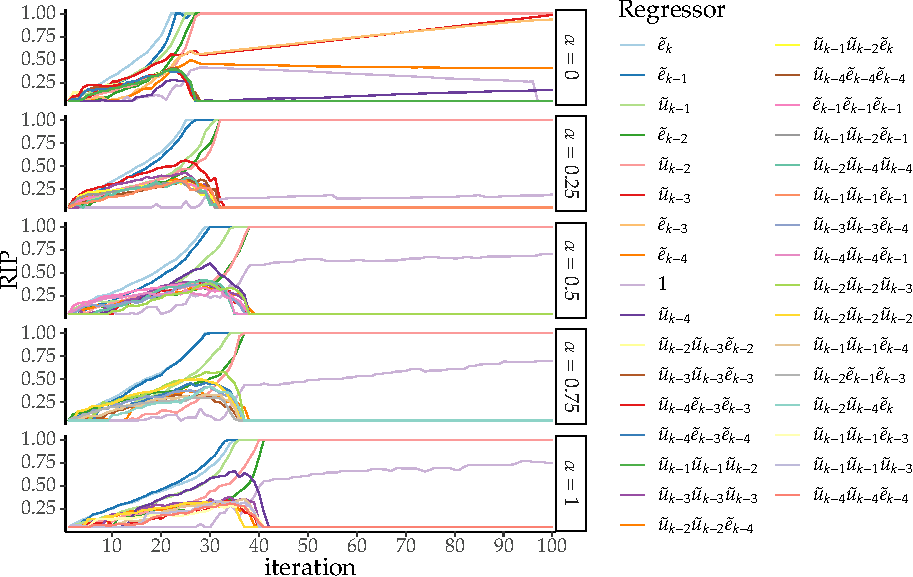
\includegraphics{Figs/Cap5/ex51_rips_evol_SR.tex.pdf}
    \caption{RIPs evolution to different values of parameter $\alpha$ considering data without noise.}
    \label{fig:exp51_ev_rips_a1_SR}
  \end{figure}
It is observed that when increasing the value of $\alpha$, regressors that do not belong to the set of ideal regressors are less frequently selected, when compared to the case where no closed loop information is used (case with $\alpha=0$) \footnote { note that the case where $\alpha=0$ in this example corresponds to case A of Example \ref{ex:sis2aord}.}.

Note that, for this realization, for $\alpha=0.5$ and $\alpha=1$ the algorithm was interrupted around iterations 60 and 90, respectively, due to the stop criterion \eqref{eq:crit.par} having been satisfied. It is emphasized that this occurs for this specific realization, the same may not happen for other realizations, due to the random character of the method.
Despite this, in general, when performing several iterations, it is possible to notice that the general behavior of Figure \ref{fig:exp51_ev_rips_a1_SR} prevails, with greater choices of spurious RIPs for the case, in which $\alpha=0$, when compared to the others ($\alpha>0$).

To analyze the behavior more generally, 50 realizations are made (with the same training data) for each value of $\alpha$. The density of probability of convergence of the RIPs for each value of $\alpha$, as a function of the number of iterations, is shown in Figure \ref{fig:exp51_dens_prob_SR}.
\begin{figure}[htpb]
  \centering
  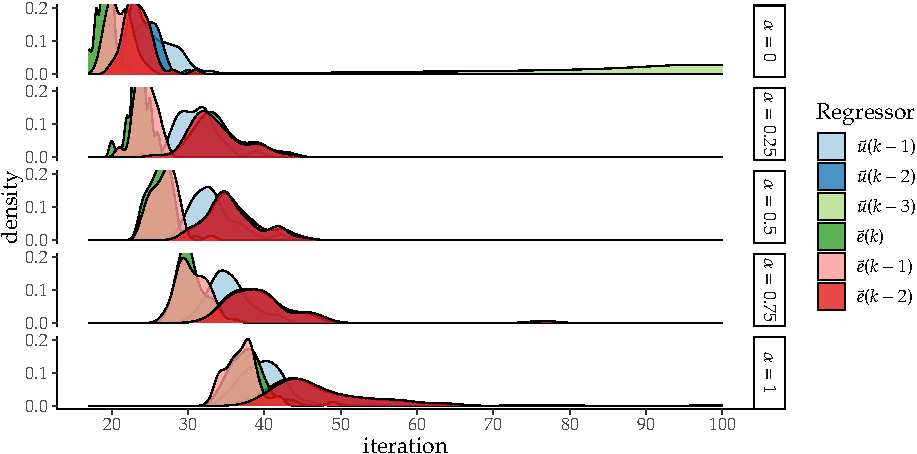
\includegraphics{Figs/Cap5/ex51_iter_con_SEM_ruido.tex.pdf}
  \caption{Probability densities of selection for the regressors selected within 100 iterations considering different values of $\alpha$ for the case without noise.}
  \label{fig:exp51_dens_prob_SR}
\end{figure}
In the figure, it is clear that the method selects the ideal parameters well for all cases. In the case without using the tracking error information, $\alpha=0$, the $\tilde{u}(k-3)$ regressor is chosen with low probability for few iterations but with increasing probability with the increase in iterations.

When tracking error information is taken into account, cases with $\alpha>0$, only the ideal regressors are selected for all 50 realizations. Note that the overall average time to choose the regressors increases with the increase in the $\alpha$ parameter. One possible explanation is that the performance index related to the tracking error, $J_r$, changes little compared to the index related to the prediction error, $J_p$. A probable solution may be to adopt a larger $K$ gain in the calculation of the MSTE (see equation \ref{eq:Jr}).

% As mesmas simulações anteriores são feitas para o caso em que existe ruído de medição (ruído na saída), como no caso B do Exemplo \ref{ex:sis2aord}. A Figura \ref{fig:exp51_ev_rips_a1_CR} mostra a evolução dos RIPs e a Figura \ref{fig:exp51_dens_prob_CR} mostra a densidade de probabilidade de escolha dos regressores em função do número de iterações para cada valor de $\alpha$, considerando esse novo caso.
The same previous simulations are done for the case in which there is measurement noise (noise at the output), as in case B of Example \ref{ex:sis2aord}. Figure \ref{fig:exp51_ev_rips_a1_CR} shows the evolution of RIPs and Figure \ref{fig:exp51_dens_prob_CR} shows the probability density of choice of regressors as a function of the number of iterations for each value of $\alpha$, considering this new case.

  \begin{figure}[htpb]
    \centering
    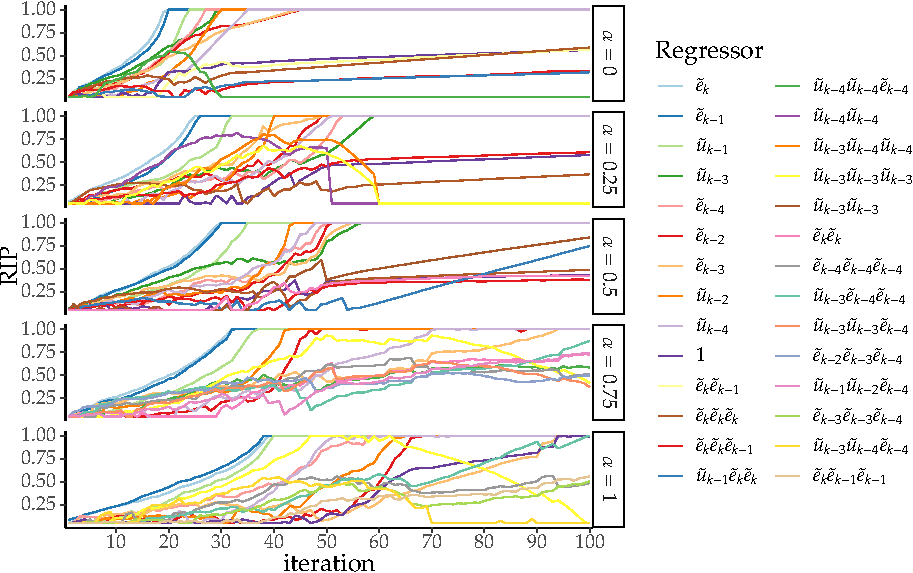
\includegraphics{Figs/Cap5/ex51_rips_evol_CR.tex.pdf}
    \caption{RIPs evolution to different values of parameter $\alpha$ considering data with noise.}
    \label{fig:exp51_ev_rips_a1_CR}
  \end{figure}

    % \footnote{note que são mostrados em cores os RIPs mais relevantes, i.e. aqueles que não convergem para $\mu_{\min}$). Estes outros são mostrados em escala de cinza e não aparecem na legenda por serem muitos (220 regressores). Os repressores ideais são mostrados em linhas mais espessas.}


  \begin{figure}[htpb]
    \centering
    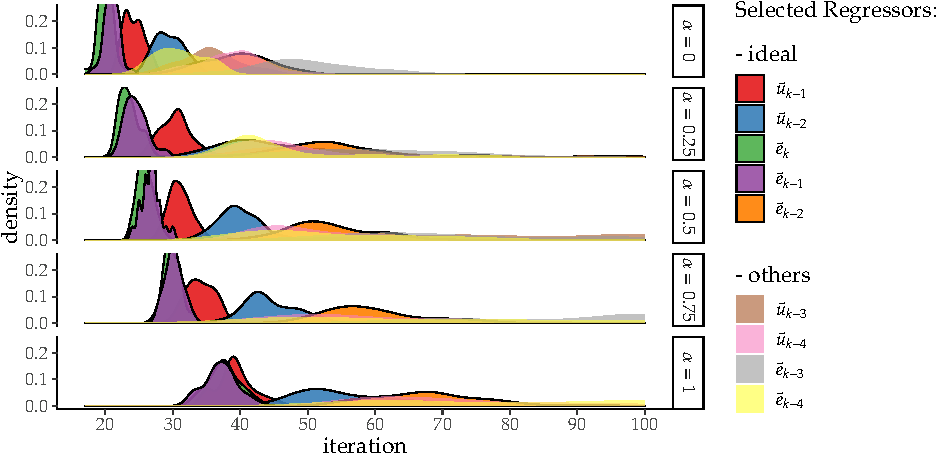
\includegraphics{Figs/Cap5/ex51_iter_con_COM_ruido.tex.pdf}
    \caption{Probability densities of selection for the regressors selected within 100 iterations considering different values of $\alpha$ for the case without noise.}
    \label{fig:exp51_dens_prob_CR}
  \end{figure}

  % Observando a Figura \ref{fig:exp51_ev_rips_a1_CR}, observa-se que os seguintes fatores: 1) em todos os casos os regressores ideais foram selecionados. Com o aumento de $\alpha$ os regressores não ideais têm uma menor densidade de probabilidade de serem escolhidos. Isto fica mais evidente comparando-se várias realizações, como mostra a Figura \ref{fig:exp51_ev_rips_a1_CR}. Comparando $\alpha=0$ com $\alpha>0$ nota-se que a probabilidade de ser selecionar regressores não ideiais diminui para menores iterações. Porém para valores maiores de $\alpha$, nota-se um maior tempo de convergência dos regressores. Por exemplo, nota-se uma quantidade maior de regressores que não convergem para o valor mínimo $\mu_{\min}$ para maiores valores de $\alpha$. O problema da polarização pode ser um dos resposponsáveis por este fator.
  Looking at Figure \ref{fig:exp51_ev_rips_a1_CR}, it is observed the following facts: 1) in all cases the ideal regressors were selected. 2) With the increase of $\alpha$, non-ideal regressors have a lower probability of being chosen. This is more evident when comparing several realizations, as shown in Figure \ref{fig:exp51_dens_prob_CR}. Comparing $\alpha=0$ with $\alpha>0$, it can be seen that the probability of selecting non-ideal regressors decreases for smaller iterations. However, for values greater than $\alpha=0$, there is a longer convergence time for the regressors. For example, we notice a greater number of regressors that do not converge to the minimum value $\mu_{\min}$ for higher values of $\alpha$. The polarization problem may be one of the factors responsible for this behavior.

  % \todo[inline]{    Neste exemplo aplico o ``RaCSS'' ao mesmo sistema de 2a ordem do exemplo anterior, mas agora usando informação do erro de rastreamento no cálculo dos RIPs. \\ Por enquanto estão somente os gráficos, ainda falta análise e algumas tabelas comparativas com ERR.  }

\end{exmp}



Nos exemplos anteriores, o algoritmo RaCSS é analisado para um caso em que o processo é linear e o controlador ideal é conhecido. Na sequência, apresenta-se um exemplo de aplicação para um processo não linear.


%!TEX root = Qualificacao.tex

\begin{exmp}[RaCSS aplicado a um sistema não-linear] \label{ex:53}

  \todo[inline]{
    Neste exemplo a ideia é avaliar o comportamento do ``RaCSS'' a um sistema não-linear. Tomei um modelo de um aquecedor com dissipação variável adotado no seu livro. A ideia é apresentado o modelo no exemplo~\ref{ex:varHeater} da seção~\ref{sec:ramss}, no sentido do RaMSS para identificar o modelo. Depois aproveito o mesmo aqui para identificar o controlador.

    Por enquanto estão somente os gráficos, ainda falta análise e algumas tabelas comparativas com ERR.
  }

  % Neste exemplo o comportamento do algoritmo RaCSS é analisado na seleção de estrutura para um sistema não linear. É adotado o modelo de um pequeno aquecedor elétrico, com dissipação variável. A variação da dissipação é resultado do acionamento de um ventilador. O sinal de entrada é a tensão elétrica aplicada ao aquecedor e a saída é o sinal amplificado de um termopar. O modelo obtido por um processo de identificação em um sistema real, conforme detalhado em \citep{aguirre2015}, seção 16.6., é dado por
  In this example, the behavior of the RaCSS algorithm is analyzed in the structure selection for a non-linear process. The model of a small electric heater, with variable dissipation, is adopted. The variation in dissipation is the result of the activation of a fan. The input signal is the electrical voltage applied to the heater and the output is the amplified signal from a thermocouple. The model obtained by an identification process in a real system, as detailed in \citep{aguirre2015}, section 16.6., Is given by
 \begin{align}
   y(k) &= 1.2929y(k-1) + 0.0101u(k-2)u(k-1) + 0.0407u^2(k-1) - 0.3779y(k-2) \\
        &\quad - 0.1280u(k-2)y(k-1) + 0.0957u(k-2)y(k-2) + 0.0051u^2(k-2)
 \label{eq:ex53_model}
 \end{align}
 
 % Os são utilizados os mesmos sinais amostrados em \ref{aguirre2015}, conforme apresentados na Figura \ref{fig:ex53_samp_data}.
 The same signals sampled presented in \cite{aguirre2015} are used to calculate the virtual values used in the RaCSS procedure. These signals are shown in Figure \ref{fig:ex53_samp_data}.
\begin{figure}[htpb]
  \centering
  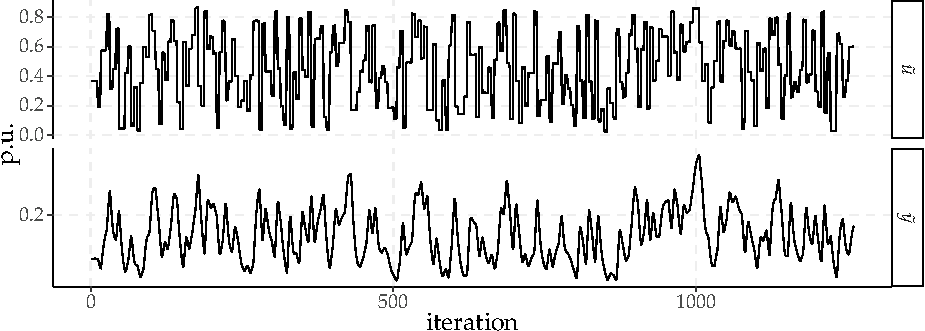
\includegraphics[width=\textwidth]{Figs/Cap5/ex53_sample_data.tex.pdf}
  \caption{Entrada e saída do aquecedor, em p.u.}
  \label{fig:ex53_samp_data}
\end{figure}
 % O período de amostragem original é de 12 segundos, porém, por simplicidade, será considerado aqui que este período de amostragem é de um segundo, $T_s =1$ s. Isto não afeta em nada os resultados a serem obtidos para fins deste exemplo numérico. Fazendo esta simplificação considera-se um modelo de referência dado por um sistema de primeira ordem, com atraso de transporte de 3 segundos e com constante de tempo de 10 segundos, resultando na seguinte função de transferência no tempo contínuo
The original sampling period is 12 seconds, however, for simplicity, it will be considered here that this sampling period is one second, $T_s =1$ s. This has no effect on the results to be obtained for the purposes of this numerical example. Making this simplification, it is considered a reference model given by a first order system, with a transport delay of 3 seconds and a time constant of 10 seconds, resulting in the following transfer function in continuous time
\begin{equation}
   M(s) = \frac{e^{-\tau_d s}}{\tau s-1},
\label{eq:}
\end{equation}
% em que $\tau = 10$ é a constante de tempo desejada e $\tau_d = 3$ é o atraso de transporte. A versão discreta deste modelo pode ser escrita como:
where $\tau = 10$ s is the desired time constant and $\tau_d = 3$ s is the transport delay. A discrete version of this model is given by
 \begin{equation}
   M(z) = \frac{1-e^{-T_s/\tau}}{(z-e^{-Ts/\tau})z^{\tau_d/Ts-1}}.
   \label{eq:ex53_MRcont}
 \end{equation}

 % Desconsiderando ruídos no processo, o procedimento RaCSS é aplicado afim de se obter um controlador que resulte em um sistema em malha fechada que se comporte de acordo com um modelo de referência dado.
 Disregarding noise in the process, the RaCSS procedure is applied in order to obtain a controller that results in a closed-loop system that behaves according to a given reference model.
 % Considera-se como regressores candidatos todos os regressores formados por monômios até 8 atrasos em $\tilde{u}$ (sinal de saída do controlador) e em $\tilde{e}$ (erro virtual).
 It is considered all regressors formed by monomials up to 8 delays in $\tilde{u}$ (controller output signal) and $\tilde{e}$ (virtual error) as candidate regressors to RaCSS.
 % Os parâmetros adotados no algorítmo RaCSS são apresentados na \ref{tab:exp53_param}, onde $\alpha$ é o fator de acoplamento dado em \eqref{eq:Jracss} e os significados dos outros símbolos são os mesmos da \ref{tab:exp51_param}.
 The parameters adopted in the RaCSS algorithm are presented in Table \ref{tab:exp53_param}, where xxxxxxxx is the factor given in \eqref{eq:Jracss} and the meanings of the other symbols are the same as presented in Table \ref{tab:exp51_param} .

\begin{table}[htpb]
  \centering
  \caption{Parameters used in the RaMSS algorithm of the example ~\ref{ex:53}}\label{tab:exp53_param}
  \begin{tabular}{c|c|c|c|c|c|c|c|c|c|c}
    $o$ & $n_{\tilde{e}}$ & $n_{\tilde{u}}$ & $ N_p$ & $ iter_{\max} $ & $K$ & $\gamma_0$ &  $\mu_{\min}$ & $\mu_{\max}$ & $\nu$ & $a$\\
    \hline
     $ 2 $ & $8$ & $8$ & $100$ & $200$ & $1$ & $2$ & $0.01$ & $1$ & $0$ & $0.5$ \\
  \end{tabular}
\end{table}

% Uma evolução típica para os RIPs, após 200 iterações é mostrada na Figura \ref{fig:ex53_rips}.
A typical evolution for the RIPs, after 200 iterations is shown in Figure \ref{fig:ex53_rips}.

  \begin{figure}[htpb]
    \centering
    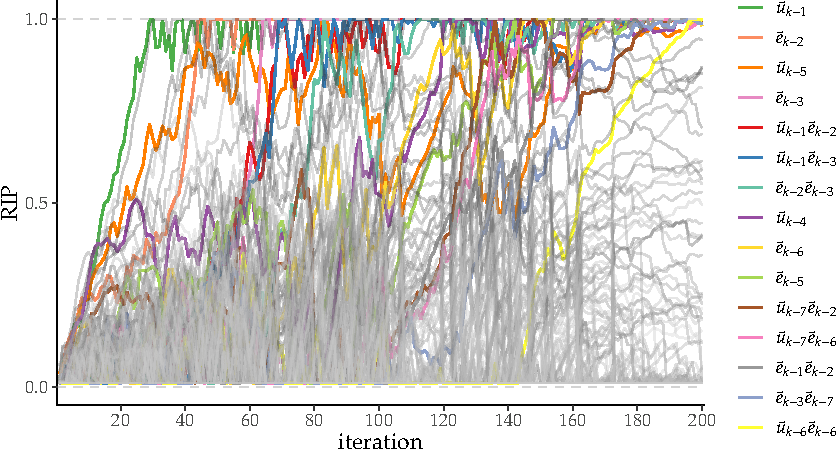
\includegraphics[width=\textwidth]{Figs/Cap5/ex53_RIPs.tex.pdf}
    \caption{RIPs evolution for example \ref{ex:53}.}
    \label{fig:ex53_rips}
  \end{figure}

  % Nota-se um comportamento bem menos regular com aqueles obtidos no Exemplo \ref{ex:52}. Ao final das 200 iterações, 15 regressores são selecionados. Apesar de ainda existirem outros regressores que ainda não convergiram para o valor mínimo e máximo, um certo grau de classificação já pode ser obtido a partir dos resultados. Ressalta-se que são um total de 171 possíveis regressores, o que resulta em um total de, aproximadamente, $2^{171}$ modelos possíveis.
  There is a much less regular behavior with those obtained in Example \ref{ex:52}. At the end of the 200 iterations, 15 regressors are selected. Although there are still other regressors that have not yet converged to the minimum and maximum value, and a certain degree of classification can already be obtained from the results. It should be noted that there are a total of 171 possible regressors, which results in a total of approximately $2^{171}$ possible models.

  % A resposta em malha fechada considerando-se os primeiros 15, 19 e 27 regressores é mostrada na Figura \ref{fig:ex31_resp_temporal}.
  The closed loop response considering the first 15, 19 and 27 regressors is shown in Figure \ref{fig:ex31_resp_temporal}.
  The MAPE, MSTE and $J_r$ index values (see \eqref{eq:MSTE} and \eqref{eq:Jracss}) are presented in Table \ref{tab:exp53_mape}.

  \begin{figure}[htpb]
  \sbox0{\blacksolidlinethin} \sbox1{\bluedashedline} \sbox2{\greendashdottedline} \sbox3{\reddashedline} \sbox4{\blackdottedline} 
    \centering
    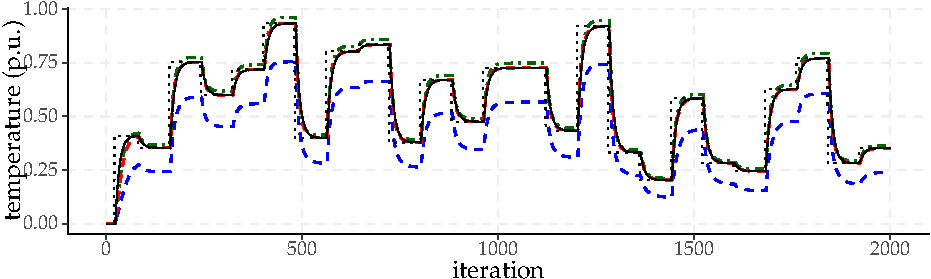
\includegraphics[width=\textwidth]{Figs/Cap5/ex53_resp_temp.tex.pdf}
    \caption{Closed loop response for controllers obtained using the first 15 (\usebox1), 19 (\usebox2) and 27 (\usebox3) RIPs obtained using RaCSS, together with the reference signal (\usebox4) and the reference model response (\usebox0).}
    \label{fig:ex31_resp_temporal}
  \end{figure}

  % Os valores do MAPE, do MSTE e do índice $J_r$ (vide \eqref{eq:MSTE} e \eqref{eq:Jracss}) são apresentados na Tabela \ref{tab:exp53_mape}.


  % Observa-se que a ao se considerar 27 regressores a resposta fica praticamente idêntica a desejada, com um valor MAPE de apenas 2.14. Nenhuma análise posterior foi feita sobre os parametros classificados. Em uma nova análise pretende-se separar os regressores selecionados e proceder novamente com o procedimento RaCSS, mas desta vez, somente com estes regressores já pré-selecionados.
  It is observed that when considering 27 regressors the answer is practically identical to the desired one, with a MAPE value of only 2.14. No further analysis was done on the classified parameters. In a new analysis, we intend to separate the selected regressors and proceed again with the RaCSS procedure, but this time, only with these pre-selected regressors.

\begin{table}[htpb]
  \centering
  \caption{Parameters used in the RaMSS algorithm of the example ~\ref{ex:53}}\label{tab:exp53_mape}
  \begin{tabular}{c|c|c|c}
     & $MAPE$ & $MSTE$ & $J_s$ \\
    \hline
    15 & 69.02 & 0.2142 & 0.8072 \\
    19 & 9.59 & 0.0050 & 0.9950 \\
    27 & 2.14 & 0.00116 & 0.9988 \\
  \end{tabular}
\end{table}


\end{exmp}





% {{{ Anotacoes

% \newpage
% \section{Rascunho}\label{sec:Rascunho}
%
%
% Como produto/trabalho em desenvolvimento durante o semestre, cita-se o trabalho que tem sido feito no sentido de desenvolver metodologias para escolha de estruturas para o controlador no âmbito do controle baseado em dados, ou DDC (Data-Driven Control).
% Mais especificamente, tem-se dado ênfase a escolha da estrutura do controlador a partir do uso de métodos VRFT.
% Como deixa claro em seu nome, ao usar o termo “sintonia” (em inglês, “tunning” ), a metodologia VR  FT visa a sintonia de um controlador pertencente a uma classe de controladores pré-estabelecida.
% Como abordado pelos autores do método~\citep{campi2002,campi2006a}, por outros estudiosos do assunto~\citep{bazanella2012} e apresentado neste relatório na seção de revisão bibliográfica, o método visa minimizar o erro de rastreamento de um modelo de referência pré-definido a partir da minimização de uma função de custo.
% Tal função é definida a partir do erro quadrático entre o sinal de excitação utilizado no processo a se controlar e o sinal de controle “virtual”, gerado pelo controlador identificado ao se aplicar  o mesmo sinal de referência capaz de produzir o mesmo sinal de saída  virtual utilizado na identificação.
%~\cite{campi2002} mostram, para o caso linear, e~\cite{campi2006}  e não linear, que ao se minimizar esta nova função de custos, minimiza-se também o erro de rastreamento, desde que se obedeça os seguintes critérios: a classe do controlador considerado tenha uma estrutura que possibilite abrigar o que se nomeia de controlador ideal (vide eq.
% ); que o processo não seja afetado por ruídos; e o controlador seja parametrizado linearmente.
% Caso o controlador ideal não possa ser representado pela classe considerada, o erro mínimo de rastreamento não é mais garantido e a introdução de um filtro ao projeto, visando se aproximar desse mínimo é desejado.
%
%
% No desenvolvimento do trabalho, foco deste relatório, tem-se feito um estudo de como seria possível, e quais as vantagens poderia-se obter se, ao invés de apenas tentar achar a melhor sintonia para um controlador com estrutura pré-estabelecida,  se procurasse também uma melhor estrutura dentro de um um conjunto de classes de controladores, de forma que o erro de rastreamento ótimo ou pelo menos sub-ótimo possa ser encontrado.
%
% Para atingir este propósito, tem-se investigado o uso de técnicas de seleção de estruturas que, com devidas adaptações e reformulações, sejam capazes selecionar modelos que resultem em controladores não lineares (ou mesmo lineares) que possam levar a respostas melhores do que aqueles que fazem uso de estruturas pré definidas.
%
% Dentre as ferramentas que têm-se utilizado, destacam-se o uso da taxa de redução de erro (ERR) e do algoritmo   Randomized Model Structure Selection (RaMSS)~\citep{falsone2014,falsone2015}. Estas estratégias têm sido estendidas e utilizadas em aplicações para determinação de modelos de processos dinâmicos~\citep{retesNARMAXModelIdentification2019} ou até mesmo no projeto de compensadores para aplicações em que o processo exibe determinados efeitos de não linearidade específicas, como no caso de efeitos histeréticos~\citep{abreuIdentificationNonlinearityCompensation2020}.

% Em particular, o método RaMSS, tem se mostrado promissor para a aplicação desejada. Esse método faz apelo às técnicas exploratórias que recorrem a buscas aleatórias ao estilo Monte Carlo, mas com mecanismos de seleção que reduzem drasticamente o custo computacional, evitando uma busca exaustiva, ao mesmo tempo em que tenta garantir uma seleção adequada.
%
% Apoiado nesta técnica, algumas adaptações têm sido estudadas no sentido de lidar agora com a identificação do controlador, e não mais do processo.
%
% Como abordado na revisão bibliográfica deste relatório, o método RaMSS faz uso de um índice de desempenho baseado no cálculo de alguma grandeza que quantifique a qualidade de o modelo em algum sentido. Uma escolha comum é calcular este índice baseado no erro quadrático médio de predição (MSPE).
%
% Um estudo sobre o uso deste índice tem sido feito na pesquisa em questão, conforme resultados apresentados na seção “Análise e Processamento de Dados”. O que se tem observado é que minimizar o MSPE diretamete pela estratégia RaMSS apesar de muitas vezes apresentar bons resultados, não dá garantias que o rastreamento ótimo é alcançado, i.e. aquele em que o erro de rastreamento médio quadrático por exemplo, é mínimo.
%
% Para sanar  esta deficiência, tem-se considerado o uso de algum índice que leve em conta o resultado final ao se aplicar os controladores intermediários identificados e selecionados pelo procedimento. Algo parecido tem sido usado no que diz respeito a identificação de processos  em que o erro quadrático médio de simulação (MSSE) é utilizado em substituição ao MSPE~\citep{aguirre2010}. Neste caso, segundo~\citep{piroddi2003}, o uso de informações da simulação-livre pode melhorar a robustez na seleção de estrutura do processo quando sob condições de identificabilidade parciais.
%
% O MSSE depende da simulação livre, que em suma é a resposta em malha aberta a um sinal de excitação conhecido. Algo parecido poderia ser utilizado ao se avaliar a estrutura no procedimento VRFT, porém, neste caso, seria desejável a resposta do sistema em malha fechada com o controlador obtido a partir da estrutura avaliada. O grande problema neste caso é que esta simulação passa a ser dependente de um modelo, ainda que aproximado do processo. Porém, como estratégias DDC visam exatamente não identificar um modelo para o processo, tal simulação torna-se inviável.
%
% No atual estágio desta pesquisa, tem-se trabalhado com a ideia de um índice que quantifique o erro médio de rastreamento em função do modelo do controlador sintonizado por uma estratégia VRFT, de modo que alguma informação da resposta em malha fechada com o controlador analisado possa ser usada para  o cálculo dos índices de probabilidades de inclusão do regressor, ou RIP (vide seção de Revisão Bibliográfica). Porém, como a simulação da resposta em malha fechada (ou mesmo malha aberta) é inviável devido a uma falta de modelo para o processo, o que se estuda é o uso de técnicas de Aprendizado por Reforço (RL) para que dados colhidos do processo real, enquanto em funcionamento, possam ser usados para o cálculo em tempo real dos RIP e consequentemente para  escolha de melhor estrutura.
%
% Algumas técnicas de RL se mostram promissoras neste caso, uma vez que muitas vezes levam à otimização de índices de desempenho a partir de dados amostrados, sem a necessidade do modelo do processo, ao mesmo tempo em que evitam o alto número de realizações amostrais como em metodologias Monte Carlo. Dentre elas a estratégia TD Learning, tem sido considerada, com uma atenção ao método conhecido como Q-learning, que permite que um controlador possa ser ajustado em uma abordagem conhecida como off-policy. Nesse caso, um controlador ou lei de controle (no caso do presente trabalho, mais precisamente sua estrutura) pode ser determinado enquanto o sistema em malha fechada obedece a uma lei (ou política) de controle diferente. Isto ajuda em eventuais problemas de instabilidade e exploração.
%
% Durante o semestre tem sido desenvolvido um algoritmo no intuito de implementar as ideiais consideradas anteriormente. Parte do algoritmo desenvolvido por Retes (2018), tem sido aproveitada, assim como algoritmos implementados e desenvolvidos pelo grupo do MACSIN1, grupo do qual o autor faz parte desde o início do doutorado. O algoritmo tem sido desenvolvido na linguagem R, portanto traduções de algumas ferramentas já disponíveis no MACSIN em outras linguagens tiveram e estão tendo que ser adaptadas. Os resultados apresentados na seção “Análise e Processamento de Dados” foram obtidos, em sua maioria, a partir deste algoritmo.


%  }}}

  \clearpage
  \thispagestyle{empty}
  \cleardoublepage
% }}} ------------------------------------------------------------------

% {{{ Capitulo 6 - Conclusoes
  % -*- TeX-master: "Qualificacao.tex" -*-
%!TEX root = Qualificacao.tex

\chapter{Conclusões}\label{cap:Concl}
\vspace{-1cm}

% Frase citação inicial {{{1
% \begin{flushright}
% \begin{minipage}{0.7\linewidth}
%     \emph{``\dots''}
% \end{minipage}
% \end{flushright}
%
% \begin{flushright}
% Cicrano
% \end{flushright}
%
%\vspace{1cm}



\section{Considerações finais}\label{sec:Cons_finais}


% Como produto/trabalho em desenvolvimento durante o semestre, cita-se o trabalho que tem sido feito no sentido de desenvolver metodologias para escolha de estruturas para o controlador no âmbito do controle baseado em dados, ou DDC (Data-Driven Control).
% Mais especificamente, tem-se dado ênfase a escolha da estrutura do controlador a partir do uso de métodos VRFT.
% Como deixa claro em seu nome, ao usar o termo “sintonia” (em inglês, “tunning” ), a metodologia VR  FT visa a sintonia de um controlador pertencente a uma classe de controladores pré-estabelecida.
% Como abordado pelos autores do método \citep{campi2002,campi2006a}, por outros estudiosos do assunto \citep{bazanella2012} e apresentado neste relatório na seção de revisão bibliográfica, o método visa minimizar o erro de rastreamento de um modelo de referência pré-definido a partir da minimização de uma função de custo.
% Tal função é definida a partir do erro quadrático entre o sinal de excitação utilizado no processo a se controlar e o sinal de controle “virtual”, gerado pelo controlador identificado ao se aplicar  o mesmo sinal de referência capaz de produzir o mesmo sinal de saída  virtual utilizado na identificação.
% \cite{campi2002} mostram, para o caso linear, e \cite{campi2006}  e não linear, que ao se minimizar esta nova função de custos, minimiza-se também o erro de rastreamento, desde que se obedeça os seguintes critérios: a classe do controlador considerado tenha uma estrutura que possibilite abrigar o que se nomeia de controlador ideal (vide eq.
% ); que o processo não seja afetado por ruídos; e o controlador seja parametrizado linearmente.
% Caso o controlador ideal não possa ser representado pela classe considerada, o erro mínimo de rastreamento não é mais garantido e a introdução de um filtro ao projeto, visando se aproximar desse mínimo é desejado.
%
%
% No desenvolvimento do trabalho, foco deste relatório, tem-se feito um estudo de como seria possível, e quais as vantagens poderia-se obter se, ao invés de apenas tentar achar a melhor sintonia para um controlador com estrutura pré-estabelecida,  se procurasse também uma melhor estrutura dentro de um um conjunto de classes de controladores, de forma que o erro de rastreamento ótimo ou pelo menos sub-ótimo possa ser encontrado.
%
% Para atingir este propósito, tem-se investigado o uso de técnicas de seleção de estruturas que, com devidas adaptações e reformulações, sejam capazes selecionar modelos que resultem em controladores não lineares (ou mesmo lineares) que possam levar a respostas melhores do que aqueles que fazem uso de estruturas pré definidas.
%
% Dentre as ferramentas que têm-se utilizado, destacam-se o uso da taxa de redução de erro (ERR) e do algoritmo   Randomized Model Structure Selection (RaMSS) \citep{falsone2014,falsone2015}. Estas estratégias têm sido estendidas e utilizadas em aplicações para determinação de modelos de processos dinâmicos \citep{retesNARMAXModelIdentification2019} ou até mesmo no projeto de compensadores para aplicações em que o processo exibe determinados efeitos de não linearidade específicas, como no caso de efeitos histeréticos \citep{abreuIdentificationNonlinearityCompensation2020}.


\section{Propostas de continuidade}\label{sec:Prop_cont}

% Como produto/trabalho em desenvolvimento durante o semestre, cita-se o trabalho que tem sido feito no sentido de desenvolver metodologias para escolha de estruturas para o controlador no âmbito do controle baseado em dados, ou DDC (Data-Driven Control).
A principal foco desta pesquisa tem sido o estudo e desenvolvimento de metodologias de projeto de controladores DDC, com foco especial na seleção de estruturas do controlador com o uso da técnica VRFT.

Em particular, o método RaMSS, tem se mostrado promissor para a aplicação desejada. Esse método faz apelo às técnicas exploratórias que recorrem a buscas aleatórias ao estilo Monte Carlo, mas com mecanismos de seleção que reduzem drasticamente o custo computacional, evitando uma busca exaustiva, ao mesmo tempo em que tenta garantir uma seleção adequada de modelos.
%
Apoiado nesta técnica, algumas adaptações têm sido estudadas no sentido de lidar com a identificação do controlador e não mais do processo.

Neste sentido, lida-se atualmente com questões que, apesar de estarem sendo abordadas no decorrer da pesquisa, resultados mais concretos ainda não foram alcançados.
Porém, as experiências e estudos têm-se mostrado promissoras, no sentido que, do ponto de vista do autor, bons resultados podem ser alcaçados.
Na sequência apresenta-se itens específicos a serem abordados, que podem ser tomados como propostas de continuidade:


Uma primeira proposta diz respeito ao estudo do uso de índices de desempenho que melhor representem a realidade do controlador ao se atualizar os termos de RIPs.
Como já abordado, originalmente o RAmSS utiliza medidas como o MSPE e MSSE para esta atualização.
Para fins de modelagem  de processos físicos, onde muitas vezes a predição do comportamento entrada-saída é o alvo, tais índices se mostram adequados \cite{falsone2015}.
%
Porém, ao se abordar o problema da idendificação do controlador, a redução do erro de predição, seja ele de passo a frente, como no caso do MSPE ou de simulação livre, como no caso do do MSSE, nem sempre é o indicativo de que haverá erro de redução de rastreamento do modelo de referência. E, para sistemas de controle, é este erro de rastreamento se torna o principal alvo em sistemas de controle.
%
% omo abordado na revisão bibliográfica deste relatório, o método RaMSS faz uso de um índice de desempenho baseado no cálculo de alguma grandeza que quantifique a qualidade de o modelo em algum sentido. Uma escolha comum é calcular este índice baseado no erro quadrático médio de predição (MSPE).
%
Um estudo sobre o uso deste índice está em andamento\todo{conforme resultados apresentados na seção ???}. O que se tem observado é que minimizar o MSPE diretamete pela estratégia RaMSS apesar de muitas vezes apresentar bons resultados\todo{não esquecer de explicar o porque destes resultados mesmo quando minimizando o MSPE, que no caso de controle fica em função dos sinais de controle e não da saída. Creio que dá para explicar isso no contexto do VRFT, em que minimizar este índice implica em minimizar o MSE de rastreamento sob certas condições.}, não dá garantias que o rastreamento ótimo é alcançado, i.e. aquele em que o erro de rastreamento médio quadrático é mínimo. 

Como alternativa, propõe-se o uso de algum índice que leve em conta o resultado em malha fechada ao se aplicar os controladores intermediários identificados e selecionados pelo procedimento. Algo parecido tem sido usado no que diz respeito a identificação de processos  em que o erro quadrático médio de simulação (MSSE) é utilizado em substituição ao MSPE \citep{aguirre2010}. Neste caso, segundo \citep{piroddi2003}, o uso de informações da simulação-livre pode melhorar a robustez na seleção de estrutura do processo quando sob condições de identificabilidade parciais.    


O MSSE depende da simulação livre, que em suma é a resposta em malha aberta a um sinal de excitação conhecido. Algo parecido poderia ser utilizado ao se avaliar a estrutura no procedimento VRFT, porém, neste caso, seria desejável a resposta do sistema em malha fechada com o controlador obtido a partir da estrutura avaliada. O grande problema neste caso é que esta simulação passa a ser dependente de um modelo, ainda que aproximado, do processo, ou do próprio processo. Porém, como estratégias DDC visam exatamente não identificar um modelo para o processo, tal situação pode ser um empecilho prático. Uma proposta de solução para este problema é apresentada mais a frente neste texto.

Uma segunda proposta, a qual também vem sendo analisada, consiste no uso de informações auxiliares durante o processo de identificação dos parâmetros do controlador.  
Apesar de já terem sido desenvolvidas técnicas para incorporar informação auxiliar no processo de identificação, por exemplo via restrições e otimização multiobjetivo \citep{barroso2006}, todas estas restrições dizem respeito à planta.
Neste sentido surgem questões como: de que forma estas técnicas podem ser usadas na abordagem DDC?
Seria possível encontrar um análogo da informação auxiliar, usada em métodos tradicionais, para estratégias DDC, em que não há informação da planta?
Poderia esta ser definida, por exemplo, a partir restrições que garantam aspectos relevantes ao controle, como limitações de ganho devido a saturação de atuadores, inserção de integradores no controlador, além de aspectos relativos a robustez? Neste sentido, um procedimento para garantir a presença de integradores no modelo do controlador já vem sendo estudado, mas ainda sem resultados conclusivos.

Outra proposta a ser estudada diz respeito ao estudo do uso de filtros no processo de identificação do controlador, como é comum na estratégia VRFT. Na estratégia, quando o controlador ideal, ou compatível, não pertence à classe de controladores considerada, ou seja, a hipótese \ref{ass:machedControl} não é satisfeita, um filtro a ser aplicado ao sinal usado no processo de identificação deve ser projetado a fim de se aproximar de uma solução ótima, conforme apresentado por \cite{campi2002,campi2006} e discutido no Capítulo \ref{cap:VRFT}.
\todo{terminar este pensamento} 

Uma quarta proposta diz respeito ao problema levantado anteriormente, onde o sinal de saída, e consequentemente o erro de rastreamento são requeridos para o cálculo do índice de atualização dos RIPs no procedimento RaMSS.
Como a simulação da resposta em malha fechada (ou mesmo malha aberta) é inviável em estratégia DDC, devido a uma falta de modelo para o processo, pretende-se fazer do uso de técnicas de Aprendizado por Reforço (RL), abordadas no Capítulo \ref{cap:RL}, para que dados colhidos do processo real, enquanto em funcionamento, possam ser usados para o cálculo em tempo real dos RIP e consequentemente para  escolha de melhor estrutura.

Algumas técnicas de RL se mostram promissoras neste caso, uma vez que muitas vezes levam à otimização de índices de desempenho a partir de dados amostrados, sem a necessidade do modelo do processo, ao mesmo tempo em que evitam o alto número de realizações amostrais como em metodologias Monte Carlo. Dentre elas a estratégia TD Learning,
\todo{Colocar referência}
tem sido considerada, com uma atenção ao método conhecido como Q-learning \cite{watkins1992}, que permite que um controlador possa ser ajustado em uma abordagem conhecida como \textit{off-policy} que permite o aprendizado de uma política de controle enquanto o sistema em malha fechada se encontra sob o efeito de outra. No âmbito deste trabalho, o sentimento é que deva ser possível o uso de uma estratégia parecida juntamente com o concito do RAmSS, possa se atualizar os RIPs e consequentemente a estrutura, e talvez até parâmetros, do controlador com um menor esforço e, se possível, com provas de convergência.

Por fim, análises a respeito de robustez, na presença de ruídos de medição ou de processos devem ser também levadas em conta, principalmente em uma etapa final. Inclusão de termos de média móvel ao procedimento RaMSS tem sido cogitado como alternativa a reduzir a polarização durante a etapa de identificação, em alternativa ao uso de estratégias baseadas em variáveis instrumentais, comuns no procedimento VRFT.



\vspace{2cm}

% No atual estágio desta pesquisa, tem-se trabalhado com a ideia de um índice que quantifique o erro médio de rastreamento em função do modelo do controlador sintonizado por uma estratégia VRFT, de modo que alguma informação da resposta em malha fechada com o controlador analisado possa ser usada para  o cálculo dos índices de probabilidades de inclusão do regressor, ou RIP (vide seção de Revisão Bibliográfica).
% Porém, como a simulação da resposta em malha fechada (ou mesmo malha aberta) é inviável devido a uma falta de modelo para o processo, o que se estuda é o uso de técnicas de Aprendizado por Reforço (RL) para que dados colhidos do processo real, enquanto em funcionamento, possam ser usados para o cálculo em tempo real dos RIP e consequentemente para  escolha de melhor estrutura.

% Algumas técnicas de RL se mostram promissoras neste caso, uma vez que muitas vezes levam à otimização de índices de desempenho a partir de dados amostrados, sem a necessidade do modelo do processo, ao mesmo tempo em que evitam o alto número de realizações amostrais como em metodologias Monte Carlo. Dentre elas a estratégia TD Learning, tem sido considerada, com uma atenção ao método conhecido como Q-learning, que permite que um controlador possa ser ajustado em uma abordagem conhecida como off-policy. Nesse caso, um controlador ou lei de controle (no caso do presente trabalho, mais precisamente sua estrutura) pode ser determinado enquanto o sistema em malha fechada obedece a uma lei (ou política) de controle diferente. Isto ajuda em eventuais problemas de instabilidade e exploração.

% Durante o semestre tem sido desenvolvido um algoritmo no intuito de implementar as ideiais consideradas anteriormente. Parte do algoritmo desenvolvido por Retes (2018), tem sido aproveitada, assim como algoritmos implementados e desenvolvidos pelo grupo do MACSIN1, grupo do qual o autor faz parte desde o início do doutorado. O algoritmo tem sido desenvolvido na linguagem R, portanto traduções de algumas ferramentas já disponíveis no MACSIN em outras linguagens tiveram e estão tendo que ser adaptadas. Os resultados apresentados na seção “Análise e Processamento de Dados” foram obtidos, em sua maioria, a partir deste algoritmo.

  \clearpage
  \thispagestyle{empty}
  \cleardoublepage

% }}} ------------------------------------------------------------------
% {{{ Captulo 6 - Resultados Experimentais
  % \input{capitulo6.tex}
  % \clearpage
  % \thispagestyle{empty}
  % \cleardoublepage
% }}} ------------------------------------------------------------------


% {{{ Bibliografia

% {{{ Para tex:
  % \bibliographystyle{rusnat}
  % \bibliography{referencias.bib}
  \bibliographystyle{apalike} % plainnat_mod
  \bibliography{refs.bib}
  % \bibliographystyle{plain}
  % \printbibheading
% % }}}

% {{{ Para biblatex:
  % \printbibliography
  % \addcontentsline{toc}{chapter}{Bibliography}
  % \clearpage
  % \thispagestyle{empty}
  % \cleardoublepage
% }}}

% }}} ------------------------------------------------------------------

% Todo's
% \listoftodos

% %Apendices
% \appendix
% \include{apendiceA}
% \clearpage
% \thispagestyle{empty}
% \cleardoublepage
% % \chapter{Algebra Linear}
% \include{apendiceB}
% \clearpage
% \thispagestyle{empty}
% \cleardoublepage
% \include{apendiceC}
% \clearpage
% \thispagestyle{empty}
% \cleardoublepage
%
% \chapter{Demonstracoes}
 %\appendix
%\include{apendiceB}
%\include{MQ}
%\include{Grubbs}

%--------------------------------------------------------------------
\end{document}

% vim: set sw=4 ts=4 sts=2 tw=80 ft=tex 

